\documentclass[11pt,a4paper,final]{article}
\usepackage[utf8]{inputenc}
\usepackage[T1]{fontenc}
\usepackage{amsmath}
\usepackage{amsfonts}
\usepackage{mathtools}
\usepackage{amssymb}
\usepackage{bm,bbm}
\usepackage[final]{graphicx}
\graphicspath{{./images/}}
\usepackage{caption}
\usepackage{subcaption}
\usepackage[usenames, dvipsnames]{color}
\usepackage[margin=1in]{geometry} % to adjust the page margins
%\pagenumbering{gobble} % To suppress page numbering 

\DeclarePairedDelimiterX{\norm}[1]{\lVert}{\rVert}{#1}
\newcommand{\seminorm}[1]{\left\lvert #1 \right\rvert}

\usepackage{tikz,pgfplots}
\pgfplotsset{table/search path={./data}} %checks in data folder
\pgfplotsset{compat=newest}	%mention version to avoid warnings
\pgfplotsset{every axis/.append style={
                    label style={font=\small},
                    legend style={font=\small, draw=none, fill=none},
                    tick label style={font=\small}
                    }}

\usepackage{array}                            % better table support
\newcolumntype{C}[1]{>{\centering\arraybackslash}m{#1}}
\usepackage{multicol}                         % spanning columns
\usepackage{multirow}                         % spanning rows
\usepackage[ruled,vlined]{algorithm2e}
\usepackage{stmaryrd} % for jump in gradient symbol
\usepackage[backend=biber,style=numeric,sorting=ynt]{biblatex}
\addbibresource{task2_ref.bib}

\begin{document}
\begin{center}
\textbf{\Large Master thesis: documentation of task 2.1}\\ \vspace{0.25cm}
\textbf{\large Vinayak Gholap}
\end{center}

\section{Tasks performed}
\begin{enumerate}
\item Understand and implement a quasi-static finite-strain elasticity problem for pure mechanical loads and deformations \cite{Pelteret2016a}, \cite{Pelteret2012}
\item Extend the application code for the axisymmetric formulation of the magneto-static magnetic scalar potential (MSP) problem to a coupled magneto-elastic problem known as a vector-valued problem
\item Implement a constitutive material law considering the geometric and material non-linearity of an isotropic continuum body \cite{Wriggers2008}
\item Implement an iterative Newton method with (quasi-static linear) load incrementing algorithm to solve the non-linear system of equations for the vector-valued solution
\item Test the developed code with mechanical toy problems that exhibit finite-strain elasticity with instability/ buckling characteristics
\end{enumerate}

\section{Quasi-static finite-strain compressible elasticity}

\subsection{Kinematics}
Consider a continuum body $\mathcal{B}_0$ in a three dimensional Euclidean space. Let any point in this reference configuration $\mathcal{B}_0$ be identified by the position vector $\mathbf{X}$. The configuration after some time $t > 0$ is termed as deformed configuration $\mathcal{B}_t$ and the corresponding position vector $\mathbf{x}$ is given by a non-linear one-to-one deformation map $\mathbf{x} = \bm{\varphi} (\mathbf{X}, t)$. The material description of the displacement of the particle at the position $\mathbf{X}$ is defined as
\begin{equation}
\mathbf{u}(\mathbf{X}, t) := \mathbf{x}(\mathbf{X}, t) - \mathbf{X}.
\end{equation}
A tensor $\mathbf{F}$ which describes the deformation process locally relates the tangent vectors of reference and current configuration to each other. It maps a material line element of the reference configuration $\bm{\mathrm{d}}\mathbf{X}$ in $\mathcal{B}_0$ to a line element $\bm{\mathrm{d}\mathbf{x}}$ in $\mathcal{B}_t$ as 
\begin{equation}
\bm{\mathrm{d}\mathbf{x}} = \mathbf{F} \cdot \bm{\mathrm{d}\mathbf{X}}.
\end{equation} 
This tensor $\mathbf{F}$ is called the deformation gradient and is the material gradient of the motion defined as
\begin{equation}
\mathbf{F}(\mathbf{X}, t) := \dfrac{\partial \bm{\varphi}(\mathbf{X}, t)}{\partial \mathbf{X}} = \nabla_0 \mathbf{x}(\mathbf{X}, t) = \mathbf{I} + \nabla_0 \mathbf{u}.
\label{eq:1.3}
\end{equation}
The gradient w.r.t. the reference configuration $\mathcal{B}_0$ is denoted as $\nabla_0$ and the gradient w.r.t. the deformed configuration $\mathcal{B}_t$ be denoted as $\nabla$ and are related as 
\begin{equation}
\nabla \{ \cdot \} = \dfrac{\partial \{ \cdot \} }{\partial \mathbf{x}} = \dfrac{\partial \{ \cdot \} }{\partial \mathbf{X}} \cdot \dfrac{\partial \mathbf{X}}{\partial \mathbf{x}} = \nabla_0 \{ \cdot \} \cdot \mathbf{F}^{-1}.
\end{equation} 
The transformation of surface area elements between $\mathcal{B}_0$ and $\mathcal{B}_t$ is given by the \textbf{Nanson's formula}
\begin{equation}
\bm{\mathrm{d}}\mathbf{a} = \mathbf{n} \cdot \mathrm{d}a = J \ \mathbf{F}^{-T} \cdot \mathbf{N} \mathrm{d}A = J \ \mathbf{F}^{-T} \cdot \bm{\mathrm{d}}\mathbf{A},
\end{equation}
where $\mathbf{n}$ is the normal vector of the surface in $\mathcal{B}_t$, $\mathbf{N}$ is the normal vector in $\mathcal{B}_0$ and $\mathrm{d}a$ and $\mathrm{d}A$ are the corresponding area elements. The determinant of the deformation gradient, known as the Jacobian, $J(\mathbf{X}, t) := \text{det} \mathbf{F}(\mathbf{X}, t) > 0$ (non-negative to avoid material self-penetration) maps the volume elements in material and spatial configurations $\mathrm{d}V$ and $\mathrm{d}v$, respectively, as 
\begin{equation}
\mathrm{d}v = J(\mathbf{X}, t) \ \mathrm{d}V.
\end{equation} 
The strain tensor in the material configuration $\mathcal{B}_0$ is defined as
\begin{equation}
\mathbf{E} := \frac{1}{2} (\mathbf{F}^T \cdot \mathbf{F} - \mathbf{I}) = \frac{1}{2} (\mathbf{C} - \mathbf{I}),
\end{equation}
and is called as the Green-Lagrange strain tensor. The tensor $\mathbf{C}:= \mathbf{F}^T \cdot \mathbf{F}$ is known as the right Cauchy-Green deformation tensor which expresses the square of the line element $\bm{\mathrm{d}}\mathbf{x}$ by the material line element $\bm{\mathrm{d}}\mathbf{X}$ as $\bm{\mathrm{d}}\mathbf{x} \cdot \bm{\mathrm{d}}\mathbf{x} = \bm{\mathrm{d}}\mathbf{X} \cdot \mathbf{C} \cdot \bm{\mathrm{d}}\mathbf{X}$. $\mathbf{C}$ is \textit{symmetric} and \textit{positive definite} at each $\mathbf{X} \in \mathcal{B}_0$. Thus the Green-Lagrange strain $\mathbf{E}$ is also symmetric. The strain $\mathbf{E}$ describes the change of the square of the line elements from $\mathcal{B}_0$ to $\mathcal{B}_t$. Using the definition of $\mathbf{F}$ from \eqref{eq:1.3}, we can express the Green-Lagrange strain in terms of the displacement gradient as 
\begin{equation}
\mathbf{E} = \frac{1}{2} ( \nabla_0 \mathbf{u} + [\nabla_0 \mathbf{u}]^T + [\nabla_0 \mathbf{u}]^T \cdot \nabla_0 \mathbf{u} ).
\end{equation}

\subsection{Kinetics}
The Cauchy stress theorem states that the Cauchy traction $\mathbf{t}$ acting on an infinitesimal surface element $\mathrm{d}a$ in the current configuration $\mathcal{B}_t$ is the product of the Cauchy stress tensor $\bm{\sigma}$, a spatial quantity, and the outward unit normal vector to the surface $\mathrm{d}a$ as 
\begin{equation}
\mathbf{t}(\mathbf{x}, t, \mathbf{n}) = \bm{\sigma}(\mathbf{x}, t) \cdot \mathbf{n}.
\end{equation}
Following the result of balance of angular momentum, it is known that the Cauchy stress tensor is symmetric. Similar relation in the material configuration is given as 
\begin{equation}
\mathbf{T}(\mathbf{X}, t, \mathbf{N}) = \mathbf{P}(\mathbf{X}, t) \cdot \mathbf{N},
\end{equation}
where $\mathbf{T}$ is the first Piola-Kirchhoff traction acting on an infinitesimal surface element $\mathrm{d}A$ and $\mathbf{P}$ is the first Piola-Kirchhoff stress tensor. $\mathbf{P}$ is a two-point tensor indicating that it is neither a material or a spatial quantity. The first Piola-Kirchhoff stress tensor is related to the Cauchy stress tensor as 
\begin{equation}
\mathbf{P} = J \ \bm{\sigma} \cdot \mathbf{F}^{-T}.
\end{equation}
The Cauchy traction $\mathbf{t}$ and the first Piola-Kirchhoff traction $\mathbf{T}$ are related as 
\begin{equation}
\mathbf{T} \ \bm{\mathrm{d}}\mathbf{A} = \mathbf{t} \ \bm{\mathrm{d}}\mathbf{a},
\end{equation}
such that
\begin{equation}
\int\limits_{\mathcal{B}_0} \left[ \mathbf{P} \cdot \mathbf{N} \right] \mathrm{d}A = \int\limits_{\mathcal{B}_0} \left[ J \ \bm{\sigma} \cdot \mathbf{F}^{-T} \right] \cdot \mathbf{N} \ \mathrm{d}A = \int\limits_{\mathcal{B}_0} \bm{\sigma} \cdot \left[ J \ \mathbf{F}^{-T} \cdot \mathbf{N} \right] \mathrm{d}A \stackrel{\text{Nanson's}}{=} \int\limits_{\mathcal{B}_t} \bm{\sigma} \cdot \mathbf{n} \ \mathrm{d}a.
\end{equation}
A completely material stress measure is also introduced known as the second Piola-Kirchhoff stress tensor given as
\begin{equation}
\mathbf{S} = \mathbf{F}^{-1} \cdot \mathbf{P}.
\end{equation}
The second Piola-Kirchhoff stress tensor is symmetric tensor.

\subsection{Constitutive material model}
\label{sec:const_law}
The kinematical relations and balance laws are not sufficient to solve a boundary value or initial value problem. For a complete set of equations, a constitutive equation needs to be formulated which can appropriately characterize the material response of a body. \par 

Hyperelastic materials are the purely elastic material behaviour under the assumption of the so-called Green elasticity. The material response is characterised by a Helmholtz free energy function $\Psi = \Psi(\mathbf{F}) = \Psi(\mathbf{C}) $ which serves as a potential for the stress. $\Psi$ describes the strain energy stored in the body and hence also known as the strain energy function (S.E.F.). When S.E.F. is described in terms of the right Cauchy-Green tensor $\mathbf{C}$ then the isotropic hyperelastic material response is 
\begin{equation}
\mathbf{S} = 2 \dfrac{\partial \Psi (\mathbf{C})}{\partial \mathbf{C}}.
\end{equation}
A Neo-Hookean solid is a hyperelastic material model that can be used for predicting the non-linear behaviour of materials undergoing large deformations under loads. The Neo-Hookean material model is usable for plastics and rubber-like materials. The S.E.F. corresponding to a compressible Neo-Hookean material is given as
\begin{equation}
\Psi \equiv \dfrac{\mu}{2} [\mathbf{C} : \mathbf{I} - \mathbf{I} : \mathbf{I} - 2 \ln J] + \dfrac{\lambda}{2} (\ln J)^2,
\label{eq:1.2}
\end{equation}
where $\mu$ and $\lambda$ are the Lam\'e parameters. For the considered S.E.F. for the Neo-Hookean material as stated in Equation \eqref{eq:1.2}, the second Piola-Kirchhoff stress is:
\begin{align}
\mathbf{S} = 2 \left\{ \dfrac{\mu}{2} \left[\dfrac{\partial (\mathbf{C} : \mathbf{I})}{\partial \mathbf{C}} - 0 - 2 \dfrac{\partial \ln J}{\partial \mathbf{C}}\right] + \dfrac{\lambda}{2} \dfrac{\partial (\ln J)^2}{\partial \mathbf{C}} \right\}
\end{align}
Employing the chain rule for the intermediate partial derivatives
\begin{align}
\dfrac{\partial (\mathbf{C} : \mathbf{I})}{\partial \mathbf{C}} &= \mathbf{I} \label{eq:1.4.1} \\ 
\dfrac{\partial \ln J}{\partial \mathbf{C}} &= \dfrac{1}{J} \dfrac{\partial J}{\partial \mathbf{C}} \label{eq:1.4.2} \\ 
\dfrac{\partial (\ln J)^2}{\partial \mathbf{C}} &= 2 \dfrac{\partial \ln J}{\partial \mathbf{C}} = 2 \dfrac{1}{J} \dfrac{\partial J}{\partial \mathbf{C}}
\label{eq:1.4.3}
\end{align}
The partial derivative of the Jacobian w.r.t. the right Cauchy-Green deformation tensor is given as \cite[see][page 46 Equation (3.124)]{Wriggers2008}:
\begin{equation}
\dfrac{\partial J}{\partial \mathbf{C}} = \dfrac{1}{2} \ J \ \mathbf{C}^{-1}.
\label{eq:1.5}
\end{equation}
Rearranging the terms with the use of the results from Equations \eqref{eq:1.4.1}, \eqref{eq:1.4.2}, \eqref{eq:1.4.3} and \eqref{eq:1.5}, we have
\begin{equation}
\mathbf{S} = \mu \mathbf{I} - \left[ \mu - \lambda \ln J \right] \mathbf{C}^{-1}.
\label{eq:1.6}
\end{equation}
The fourth-order elasticity tensor in the material description is defined as 
\begin{equation}
\mathfrak{C} := 2 \dfrac{\partial \mathbf{S}(\mathbf{C})}{\partial \mathbf{C}} = 4 \dfrac{\partial^2 \Psi (\mathbf{C})}{\partial \mathbf{C} \otimes \partial \mathbf{C}}.
\label{eq:1.6.2}
\end{equation}
Using the derived form for the second Piola-Kirchhoff stress from Equation \eqref{eq:1.6}, we have
\begin{equation}
\mathfrak{C} = \left[ 2 \lambda \ln J - 2 \mu \right]\dfrac{\partial \mathbf{C}^{-1}}{\partial \mathbf{C}} + \lambda \mathbf{C}^{-1} \otimes \mathbf{C}^{-1},
\end{equation}
with the standard result \cite[see][page 519]{Wriggers2008}
\begin{equation}
\dfrac{\partial C^{-1}_{IJ}}{\partial C_{KL}} := \dfrac{-1}{2} \left[ C^{-1}_{IK} \ C^{-1}_{LJ} + C^{-1}_{IL} \ C^{-1}_{KJ} \right].
\end{equation}
The fourth-order elasticity tensor for hyperelastic materials possess both major and minor symmetries, i.e. $\mathfrak{C} = C_{IJKL} = C_{KLIJ} = C_{JIKL} = C_{IJLK}$.

\section{Weak formulation in the referential configuration}
For the analysis of (non-)linear initial boundary value problems in continuum theory, a coupled system of partial differential equations needs to be solved consisting of kinematical relations, the local balance law of linear momentum and the constitutive equations. The description of the strong form of these equations, here, will be with respect to the initial configuration of the bodies. 
\begin{align*}
\text{Kinematics}&: \ \mathbf{F}, \ \mathbf{E} = \dfrac{1}{2} (\mathbf{F}^T \cdot \mathbf{F} - \mathbf{I}) \\
\text{Equilibrium}&: \ \text{Div}(\mathbf{F} \cdot \mathbf{S}) + \mathbf{b}^p = \mathbf{0} \\
\text{Constitutive equation}&: \ \mathbf{S} = 2\dfrac{\partial \Psi}{\partial \mathbf{C}}.
\end{align*}
In addition the boundary conditions for the displacements have to be imposed on $\partial \mathcal{B}_{0,u}$ and for tractions on the boundary $\partial \mathcal{B}_{0,t}$, with $\partial \mathcal{B}_{0,u} \cap \partial \mathcal{B}_{0,t} = \emptyset$.
\begin{equation*}
\text{Boundary conditions} : \ \mathbf{u} = \mathbf{u}^p \ \text{on} \ \partial \mathcal{B}_{0,u} \ \& \ \mathbf{F} \cdot \mathbf{S} \cdot \mathbf{N} = \mathbf{t}^p \ \text{on} \ \partial \mathcal{B}_{0,t}.
\end{equation*}
$\mathbf{b}^p$ is the prescribed body force and $\mathbf{t}^p$ is the prescribed traction force per unit area. The finite element method, which is based on a variational formulation of the equations, can be fulfilled in a weak sense minimizing the error of the finite element approximation for arbitrarily chosen test functions. Let $\mathbf{u}^h$ be the approximation of the exact solution $\mathbf{u}$. Since the approximate solution is usually not the same as the exact solution, an error $\mathbf{R}$ will occur when satisfying the strong form of the above equations.
\begin{equation}
\text{Div}(\mathbf{F}(\mathbf{u}^h) \cdot \mathbf{S}) + \mathbf{b}^p = \mathbf{R}.
\end{equation}
The error $\mathbf{R}$ will be minimized in a weak sense by multiplying the residual by a vector-valued weighting function $\bm{\eta}$ and integrating the residual over the whole domain. This vector-valued function $\bm{\eta}$ is called as test function. Thus, we have
\begin{equation}
\int\limits_{\mathcal{B}_0} \text{Div}(\mathbf{F} \cdot \mathbf{S}) \cdot \bm{\eta} \ \mathrm{d}V + \int\limits_{\mathcal{B}_0} \mathbf{b}^p \cdot \bm{\eta} \ \mathrm{d}V = 0 \ \ \forall \bm{\eta}.
\label{eq:1.7}
\end{equation}
By doing integration by parts of the first term in Equation \eqref{eq:1.7}, with the application of divergence theorem and the boundary conditions for displacement and traction, we have the weak form as 
\begin{equation}
\int\limits_{\mathcal{B}_0} \mathbf{F} \cdot \mathbf{S} \cdot \nabla_0 \bm{\eta} \ \mathrm{d}V - \int\limits_{\mathcal{B}_0} \mathbf{b}^p \cdot \bm{\eta} \ \mathrm{d}V - \int\limits_{\mathcal{\partial B}_{0,t}} \mathbf{t}^p \cdot \bm{\eta} \ \mathrm{d}A = 0 \ \ \forall \bm{\eta}.
\label{eq:1.8}
\end{equation}
Simplifying the first term in Equation \eqref{eq:1.8} using the fact that the scalar product of a symmetrical tensor with an anti-symmetrical tensor is zero, we have
\begin{align}
\mathbf{F} \cdot \mathbf{S} \cdot \nabla_0 \bm{\eta} = \mathbf{S} \cdot \mathbf{F}^T \cdot \nabla_0 \bm{\eta} = \mathbf{S} \cdot \dfrac{1}{2} (\mathbf{F}^T \cdot \nabla_0 \bm{\eta} + \nabla_0^T \bm{\eta} \cdot \mathbf{F}) = \mathbf{S} \cdot \delta \mathbf{E}.
\label{eq:1.9}
\end{align}
$\delta \mathbf{E}$ denotes the variation of the Green-Lagrange strain tensor which is obtained as the directional derivative
\begin{align}
D\mathbf{E} \cdot \bm{\eta} &= \dfrac{1}{2} \dfrac{\mathrm{d}}{\mathrm{d\alpha}} \left[ \mathbf{F}^T (\bm{\varphi} + \alpha \bm{\eta}) \cdot \mathbf{F}(\bm{\varphi} + \alpha \bm{\eta}) - \mathbf{I} \right] \Big|_{\alpha = 0} \nonumber \\
&= \dfrac{1}{2} \left[ \dfrac{\partial \mathbf{F}^T (\bm{\varphi} + \alpha \bm{\eta})}{\partial \alpha} \cdot \mathbf{F}(\bm{\varphi} + \alpha \bm{\eta}) + \mathbf{F}^T (\bm{\varphi} + \alpha \bm{\eta}) \cdot \dfrac{\partial \mathbf{F}(\bm{\varphi} + \alpha \bm{\eta})}{\partial \alpha} - \dfrac{\partial \mathbf{I}}{\partial \alpha} \right] \Bigg|_{\alpha = 0} \nonumber \\
&= \dfrac{1}{2} \left[ \dfrac{\partial \left[ \mathbf{I} + \nabla_0^T (\bm{\varphi} + \alpha \bm{\eta}) \right]}{\partial \alpha} \cdot \mathbf{F}(\bm{\varphi} + \alpha \bm{\eta}) + \mathbf{F}^T (\bm{\varphi} + \alpha \bm{\eta}) \cdot \dfrac{\partial \left[ \mathbf{I} + \nabla_0 (\bm{\varphi} + \alpha \bm{\eta}) \right]}{\partial \alpha} - \mathbf{0} \right] \Bigg|_{\alpha = 0} \nonumber \\
&\stackrel{\alpha = 0}{=} \dfrac{1}{2} \left[ (\nabla_0 \bm{\eta})^T \cdot \mathbf{F} (\bm{\varphi}) + \mathbf{F}^T (\bm{\varphi}) \cdot \nabla_0 \bm{\eta} \right] = \delta \mathbf{E}.
\label{eq:1.10}
\end{align}
Using the result of Equation \eqref{eq:1.9} and Equation \eqref{eq:1.10} in Equation \eqref{eq:1.8}, we have
\begin{equation}
G(\bm{\varphi},\bm{\eta}):= \int\limits_{\mathcal{B}_0} \mathbf{S} \cdot \delta \mathbf{E} \ \mathrm{d}V - \int\limits_{\mathcal{B}_0} \mathbf{b}^p \cdot \bm{\eta} \ \mathrm{d}V - \int\limits_{\mathcal{\partial B}_{0,t}} \mathbf{t}^p \cdot \bm{\eta} \ \mathrm{d}A = 0 \ \ \forall \bm{\eta}.
\label{eq:1.11}
\end{equation}
The first term in Equation \eqref{eq:1.11} denotes the internal virtual work performed by the body. The last two terms are the virtual work of the applied traction and the inertia load.

\subsection{Variational principles}
\textbf{Principle of stationary potential energy}: The S.E.F. for the considered hyperelastic material model describes the stored energy in the continuum body. Based on this S.E.F. we can find the equilibrium configuration by the principle of minimum potential energy. The total potential energy of the system $\Pi$ is the sum of the internal and external potential energies and is defined as 
\begin{equation}
\Pi = \Pi_{int} + \Pi_{ext},
\label{eq:1.12}
\end{equation}
where 
\begin{align}
\Pi_{int} &= \int\limits_{\mathcal{B}_0} \Psi (\mathbf{C}) \ \mathrm{d}V \\
\Pi_{ext} &= - \int\limits_{\mathcal{B}_0} \mathbf{b}^p \cdot \bm{\varphi} \ \mathrm{d}V - \int\limits_{\mathcal{\partial B}_{0,t}} \mathbf{t}^p \cdot \bm{\varphi} \ \mathrm{d}A.
\end{align}
The value of $\bm{\varphi}$ which makes $\Pi$ stationary satisfies the equilibrium configuration, i.e. find $\bm{\varphi}$ such that $\min\limits_{\bm{\varphi}} \Pi \to \text{stat.}$. The stationary value of Equation \eqref{eq:1.12} is found by the variation of $\Pi$ w.r.t. the deformation
\begin{align}
\delta \Pi = D \Pi \cdot \bm{\eta} &= \dfrac{\partial \Pi}{\partial \mathbf{u}} \cdot \delta \mathbf{u} =: R(\mathbf{u}; \delta \mathbf{u})\nonumber \\
&= \int\limits_{\mathcal{B}_0} \dfrac{\partial \Psi (\mathbf{C})}{\partial \mathbf{C}} \cdot D \mathbf{C} \cdot \bm{\eta} \ \mathrm{d}V - \int\limits_{\mathcal{B}_0} \mathbf{b}^p \cdot \delta \mathbf{u} \ \mathrm{d}V - \int\limits_{\mathcal{\partial B}_{0,t}} \mathbf{t}^p \cdot \delta \mathbf{u} \ \mathrm{d}A = 0
\end{align}
with 
\begin{equation}
\dfrac{\partial \Psi (\mathbf{C})}{\partial \mathbf{C}} = \dfrac{1}{2} \mathbf{S} \ \ \text{and} \ \ D \mathbf{C} \cdot \bm{\eta} = 2 \ D \mathbf{E} \cdot \bm{\eta} = 2 \delta \mathbf{E}
\label{eq:1.12.2}
\end{equation}
\begin{align}
R(\mathbf{u}; \delta \mathbf{u}) =\delta \Pi = \int\limits_{\mathcal{B}_0} \mathbf{S} \cdot \delta \mathbf{E} \ \mathrm{d}V - \int\limits_{\mathcal{B}_0} \mathbf{b}^p \cdot \delta \mathbf{u} \ \mathrm{d}V - \int\limits_{\mathcal{\partial B}_{0,t}} \mathbf{t}^p \cdot \delta \mathbf{u} \ \mathrm{d}A = 0 
\label{eq:1.13}
\end{align}
Hence the variational form $R(\mathbf{u}; \delta \mathbf{u})$ in Equation \eqref{eq:1.13} is equivalent to the weak form $G(\bm{\varphi},\bm{\eta})$ in Equation \eqref{eq:1.11} when the material energy is defined by a strain energy function. 

\section{Linearizations}
The variational form $R$ in Equation \eqref{eq:1.13} is a non-linear equation. Geometrical non-linearity occurs due to the non-linear Green-Lagrange strain tensor. Linearizations of the associated non-linear terms is necessary in the algorithmic treatment of the solution process for the non-linear boundary value problems. Assuming the state of the system is known at some load or time step $t_{n-1}$, the linearization of the non-linear residual $R$ by an iterative solution method (such as Newton-Raphson) is given as: Find increment $\Delta \mathbf{u}$ such that 
\begin{equation}
\mathbf{L}\left[ R \right]_{\mathbf{u}_{i+1} = \mathbf{u}_{i} + \Delta \mathbf{u}_i} \ = \ R(\mathbf{u}_{i}) + D_{\Delta\mathbf{u}} R(\mathbf{u}_i; \delta \mathbf{u}) \cdot \Delta\mathbf{u} = R(\mathbf{u}_{i}) + D^2_{\Delta\mathbf{u}, \delta\mathbf{u}} \Pi(\mathbf{u}_{i}) \cdot \Delta\mathbf{u} = 0,
\label{eq:1.14}
\end{equation}
where, the value of a quantity at the current iteration $i$ under an iterative solver regime is denoted as ${\left\lbrace \cdot \right\rbrace}_{i}^{n} = {\left\lbrace \cdot \right\rbrace}_{i}$ at the currently unknown state $t_n$ (i.e. the load or time step at $n$). The incremental change between iterative solver iterations $i$ and $i+1$ is denoted as $\Delta \left\lbrace \cdot \right\rbrace := {\left\lbrace \cdot \right\rbrace}_{i+1} - {\left\lbrace \cdot \right\rbrace}_{i}$. \par 

After a certain convergence criteria is reached at each Newton step, we update the solution at the current load step $t_n$ as $\mathbf{u}_{i+1} = \mathbf{u}_i + \Delta \mathbf{u}$. The tangent matrix $\mathbf{K}$ in Equation \eqref{eq:1.14} is given as 
\begin{equation}
D^2_{\Delta\mathbf{u}, \delta\mathbf{u}} \Pi(\mathbf{u}_{i}) = D_{\Delta\mathbf{u}} R(\mathbf{u}_i; \delta \mathbf{u}) \cdot \Delta\mathbf{u} =: \mathbf{K}(\mathbf{u}_i; \Delta\mathbf{u}, \delta \mathbf{u}).
\end{equation}
Assuming dead loading for the sake of simplicity to derive the tangent matrix, i.e. the body load and traction do not change due to the deformation of the body, we have
\begin{align}
\mathbf{K}(\mathbf{u}_i; \Delta\mathbf{u}, \delta \mathbf{u}) = \int\limits_{\mathcal{B}_0} D_{\Delta\mathbf{u}} \left[ \mathbf{S} \cdot \delta \mathbf{E} \right] \cdot \Delta\mathbf{u} \ \mathrm{d}V.
\label{eq:1.15}
\end{align}
The kinematical quantity Green-Lagrange strain $\mathbf{E}$ and the constitutive relation quantity second Piola-Kirchhoff stress tensor $\mathbf{S}$ are non-linear tensors. In order to form a system of linear equations from Equation \eqref{eq:1.15} and the solution of it, we require the linearized forms of the non-linear terms $\mathbf{E}$ and $\mathbf{S}$.
\subsection{\textbf{Basic concept of linearization process}}
To demonstrate the basic idea of linearizations for non-linear problems, consider a non-linear $C^1$ mapping $\mathbf{G}: \mathcal{E} \mapsto \mathcal{F}$, where $\overline{\mathbf{x}}$ and $\Delta\mathbf{x}$ are points of the abstract space $\mathcal{E}$. The elements of the spaces $\mathcal{E}$ and $\mathcal{F}$ can be scalar-, vector- or tensor-fields. The Taylor series expansion of this mapping about a point $\overline{\mathbf{x}} + \Delta\mathbf{x}$ is given as
\begin{equation}
\mathbf{G}(\overline{\mathbf{x}} + \Delta\mathbf{x}) = \mathbf{G}(\overline{\mathbf{x}}) + D \mathbf{G}(\overline{\mathbf{x}}) \cdot \Delta\mathbf{x} + \mathbf{R}.
\end{equation}
The term $\mathbf{R}$ refers to the higher-order truncated terms. The linear part of the mapping $\mathbf{G}$ at $\overline{\mathbf{x}}$ is 
\begin{equation}
\mathbf{L} \left[ \mathbf{G} \right]_{\mathbf{x} = \overline{\mathbf{x}}} = \mathbf{G}(\overline{\mathbf{x}}) + D \mathbf{G}(\overline{\mathbf{x}}) \cdot \Delta\mathbf{x}.
\end{equation} 
Thus, the first-order Taylor series expansion corresponds to the linearization of the weak form in the finite element applications. 
\subsection{\textbf{Linearization of Kinematical quantity}}
The linearization of the variation of Green-Lagrange strain tensor is 
\begin{equation}
\mathbf{L}\left[ \mathbf{E} \right] = \mathbf{E}(\overline{\bm{\varphi}}) + D \mathbf{E}(\bm{\varphi}) \cdot \Delta \mathbf{u},
\label{eq:1.17}
\end{equation}
where the directional derivative in the direction of increment $\Delta \mathbf{u}$ is given as in the result of Equation \eqref{eq:1.10}
\begin{equation}
D \mathbf{E}(\bm{\varphi}) \cdot \Delta\mathbf{u} = \dfrac{1}{2} \left[ \Delta(\nabla_0^T \mathbf{u}) \cdot \mathbf{F} + \mathbf{F}^T \cdot \Delta(\nabla_0 \mathbf{u}) \right] = \Delta \mathbf{E},
\label{eq:1.18}
\end{equation}
with $\Delta\mathbf{E}$ being the increment of the Green-Lagrange deformation tensor.
\subsection{\textbf{Linearization of Constitutive equation}}
The constitutive equation for the hyperelastic Neo-Hookean material model in Section \eqref{sec:const_law} was derived in terms of the right Cauchy-Green deformation tensor $\mathbf{C}$ and thus the second Piola-Kirchhoff stress tensor also depends on $\mathbf{C}$. The linearization of $\mathbf{S}$ is
\begin{align}
\mathbf{L}\left[ \mathbf{S} \right]_{\bm{\varphi} = \overline{\bm{\varphi}}} \ &= \ \mathbf{S}(\overline{\bm{\varphi}}) + D \mathbf{S}(\bm{\varphi}) \cdot \Delta\mathbf{u} \nonumber \\
&= \ \mathbf{S}(\overline{\bm{\varphi}}) + \dfrac{\partial \mathbf{S}}{\partial \mathbf{C}} \Big|_{\bm{\varphi} = \overline{\bm{\varphi}}} : \left[ D \mathbf{C}(\overline{\bm{\varphi}}) \cdot \Delta\mathbf{u} \right].
\label{eq:1.16}
\end{align}
Using the results of Equation \eqref{eq:1.6.2} and Equation \eqref{eq:1.12.2} in Equation \eqref{eq:1.16}, we get
\begin{equation}
\mathbf{L}\left[ \mathbf{S} \right]_{\bm{\varphi} = \overline{\bm{\varphi}}} \ = \mathbf{S}(\overline{\bm{\varphi}}) + \mathfrak{C}(\overline{\bm{\varphi}}) : \left[ \Delta \mathbf{E}(\overline{\bm{\varphi}}) \right]
\label{eq:1.19}
\end{equation} \newline 
The first term in Equation \eqref{eq:1.19} is Equation \eqref{eq:1.9} with $\mathbf{F}$ and $\mathbf{S}$ evaluated at the fixed point $\overline{\bm{\varphi}}$ instead of $\bm{\varphi}$. With the assumption that the applied load is conservative, the directional derivative in Equation \eqref{eq:1.14} can be computed by taking only the first term in Equation \eqref{eq:1.9} into account
\begin{align}
D_{\Delta\mathbf{u}} R(\mathbf{u}_i; \Delta \mathbf{u}) \cdot \Delta\mathbf{u} &= \int\limits_{\mathcal{B}_0} \left[ D \{ \mathbf{F}(\overline{\bm{\varphi}}) \cdot \mathbf{S}(\overline{\bm{\varphi}})\} \cdot \Delta\mathbf{u} \right] \cdot \nabla_0 \delta\mathbf{u} \ \mathrm{d}V \ \ \forall \delta\mathbf{u} \nonumber \\
&= \int\limits_{\mathcal{B}_0} \Big\lbrace \nabla_0 (\Delta\mathbf{u}) \cdot \mathbf{S}(\overline{\bm{\varphi}}) + \mathbf{F}(\overline{\bm{\varphi}}) \cdot \left[ D \mathbf{S}(\overline{\bm{\varphi}}) \cdot \Delta\mathbf{u} \right] \Big\rbrace \cdot \nabla_0 \delta\mathbf{u} \ \mathrm{d}V \ \ \forall \delta\mathbf{u}
\label{eq:1.20}
\end{align}
The directional derivative of $\mathbf{S}$ at $\overline{\bm{\varphi}}$ as taken from the linearization of constitutive equation in Equation \eqref{eq:1.19} is 
\begin{equation}
D \mathbf{S}(\overline{\bm{\varphi}}) \cdot \Delta\mathbf{u} = \mathfrak{C}(\overline{\bm{\varphi}}) : \left[ \Delta \mathbf{E}(\overline{\bm{\varphi}}) \right],
\label{eq:1.21}
\end{equation}
where $\Delta \mathbf{E}$ is the linearization of kinematical quantity from Equation \eqref{eq:1.18} evaluated at the fixed point $\overline{\bm{\varphi}}$.  Substituting Equation \eqref{eq:1.21} in Equation \eqref{eq:1.20} and by using the symmetry of $\mathfrak{C}$ along with the result of Equation \eqref{eq:1.10}, we have the final linearized form of the variational formulation as
\begin{equation}
D_{\Delta\mathbf{u}} R(\mathbf{u}_i; \Delta \mathbf{u}) \cdot \Delta\mathbf{u} = \int\limits_{\mathcal{B}_0} \Big\lbrace \nabla_0 (\Delta\mathbf{u}) \cdot \mathbf{S}(\overline{\bm{\varphi}}) \cdot \nabla_0 \delta \mathbf{u} + \delta \mathbf{E}(\overline{\bm{\varphi}}) \cdot \mathfrak{C}(\overline{\bm{\varphi}}) : \left[ \Delta\mathbf{E}(\overline{\bm{\varphi}}) \right] \Big\rbrace \ \mathrm{d}V \ \ \forall \delta\mathbf{u}.
\label{eq:1.22}
\end{equation}
The final linearized form is symmetric in $\delta\mathbf{u}$ and $\Delta\mathbf{u}$. The first term in Equation \eqref{eq:1.22} is known as \textit{the geometrical tangent} due to the direct appearance of stress at the given state. The second term is known as \textit{the material tangent} since it contains along with the incremental constitutive tensor $\mathfrak{C}$, the variation $\delta \mathbf{E} := \dfrac{1}{2} \Big(\left[\nabla_0 \delta\mathbf{u} \right]^T \cdot \mathbf{F}(\overline{\bm{\varphi}}) + \mathbf{F}^T (\overline{\bm{\varphi}}) \cdot \nabla_0 \delta\mathbf{u} \Big)$ and the increment $\Delta \mathbf{E} := \dfrac{1}{2} \Big(\left[\nabla_0 \Delta\mathbf{u}\right]^T \cdot \mathbf{F}(\overline{\bm{\varphi}}) + \mathbf{F}^T (\overline{\bm{\varphi}}) \cdot \nabla_0 \Delta\mathbf{u} \Big)$ of the Green-Lagrange strain tensor.  
 
\section{Discretization by the finite element method}
For the considered linearized weak formulation at Newton increment $i$ and time step $t_n$ from Equation \eqref{eq:1.14}
\begin{equation}
D_{\Delta \mathbf{u}} R(\mathbf{u}_i; \Delta \mathbf{u}) \cdot \Delta\mathbf{u} = -R(\mathbf{u}_{i}) ,
\label{eq:1.24}
\end{equation}
with the tangent matrix and the residual evaluated at $\overline{\bm{\varphi}} = \bm{\varphi}(t_n,i)$ given by
\begin{align*}
D_{\Delta\mathbf{u}} R(\mathbf{u}_i; \Delta \mathbf{u}) \cdot \Delta\mathbf{u} &= \int\limits_{\mathcal{B}_0} \Big\lbrace \nabla_0 (\Delta\mathbf{u}) \cdot \mathbf{S}(\overline{\bm{\varphi}}) \cdot \nabla_0 \delta\mathbf{u} + \delta \mathbf{E}(\overline{\bm{\varphi}}) \cdot \left[ \mathfrak{C}(\overline{\bm{\varphi}}) : \Delta\mathbf{E}(\overline{\bm{\varphi}}) \right] \Big\rbrace \ \mathrm{d}V \ \ \forall \delta\mathbf{u} \\
\text{and} \ \ R(\mathbf{u}_i; \Delta \mathbf{u}) &= \int\limits_{\mathcal{B}_0} \mathbf{S}(\overline{\bm{\varphi}}) \cdot \delta \mathbf{E}(\overline{\bm{\varphi}}) \ \mathrm{d}V,
\end{align*}
we can now discretize it using the finite element approximation: find $\mathbf{u} \in \mathbf{W} = H^1_0 (\mathcal{B}_0; \mathbb{R}^{\text{dim}})$ such that for all $\delta\mathbf{u} \in \mathbf{V} = H^1 (\mathcal{B}_0; \mathbb{R}^{\text{dim}})$ it holds
\begin{equation}
\int\limits_{\mathcal{B}_0} \Big\lbrace \nabla_0 (\Delta\mathbf{u}) \cdot \mathbf{S}(\overline{\bm{\varphi}}) \cdot \nabla_0 \delta\mathbf{u} + \delta \mathbf{E}(\overline{\bm{\varphi}}) \cdot \left[ \mathfrak{C}(\overline{\bm{\varphi}}) : \Delta\mathbf{E}(\overline{\bm{\varphi}}) \right] \Big\rbrace \ \mathrm{d}V = -\int\limits_{\mathcal{B}_0} \mathbf{S}(\overline{\bm{\varphi}}) \cdot \delta \mathbf{E}(\overline{\bm{\varphi}}) \ \mathrm{d}V \ \ \forall \delta\mathbf{u}.
\label{eq:1.23}
\end{equation}
The Sobolev space is given as 
\begin{equation}
H^1 = \Big\lbrace \mathbf{u}: \Omega \mapsto \mathbb{R} \Bigg| \int\limits_{\Omega} \norm{\mathbf{u}}^2 + \norm{\nabla \mathbf{u}}^2 \ \mathrm{d}\Omega < \infty \Big\rbrace.
\end{equation}
The vector-valued function spaces are given as 
\begin{align}
\mathbf{W} &= \left\lbrace \mathbf{u} \in H^1, \mathbf{u} \big|_{\partial \Omega_D} = \overline{\mathbf{u}} \right\rbrace, \\
\mathbf{V} &= \left\lbrace \delta\mathbf{u} \in H^1, \delta\mathbf{u} \big|_{\partial \Omega_D} = \mathbf{0} \right\rbrace.
\end{align}
The approximates in the discrete function spaces $\mathbf{W}^h \subset \mathbf{W}$ and $\mathbf{V}^h \subset \mathbf{V}$ is given as a linear combination of $M$ vector-valued shape functions
\begin{align}
\mathbf{W}^h &= \left\lbrace \mathbf{u}^h \in \mathbf{W} : \mathbf{u}^h (\mathbf{x}) = \sum\limits_{I=1}^{M} u_I \ \mathbf{N}_I (\mathbf{x}), \ u_I \in \mathbb{R} \right\rbrace, \nonumber\\
\mathbf{V}^h &= \left\lbrace \delta\mathbf{u}^h \in \mathbf{V} : \delta\mathbf{u}^h (\mathbf{x}) = \sum\limits_{J=1}^{M} \delta u_J \ \mathbf{N}_J (\mathbf{x}), \ \delta u_J \in \mathbb{R} \right\rbrace.
\end{align}
The increments, derivatives and derivatives of increments of the functions in the function space $\mathbf{W}^h$ are given as
\begin{align}
\Delta\mathbf{W}^h &= \left\lbrace \Delta\mathbf{u}^h \in \mathbf{W} : \Delta\mathbf{u}^h (\mathbf{x}) = \sum\limits_{I=1}^{M} \Delta u_I \ \mathbf{N}_I (\mathbf{x}), \ \Delta u_I \in \mathbb{R} \right\rbrace, \\
\nabla\mathbf{W}^h &= \left\lbrace \nabla\mathbf{u}^h \in \mathbf{W} : \nabla\mathbf{u}^h (\mathbf{x}) = \sum\limits_{I=1}^{M} u_I \ \nabla\mathbf{N}_I (\mathbf{x}), \ u_I \in \mathbb{R} \right\rbrace, \\
\nabla \Delta\mathbf{W}^h &= \left\lbrace \nabla \Delta\mathbf{u}^h \in \mathbf{W} : \nabla \Delta\mathbf{u}^h (\mathbf{x}) = \sum\limits_{I=1}^{M} \Delta u_I \ \nabla\mathbf{N}_I (\mathbf{x}), \ \Delta u_I \in \mathbb{R} \right\rbrace.
\end{align}
Inserting the descritized approximations $\Delta \mathbf{u}\approx \Delta \mathbf{u}^h$ and $\delta \mathbf{u} \approx \delta \mathbf{u}^h$ in Equation \eqref{eq:1.23}, we have
\begin{align}
&\int\limits_{\mathcal{B}_0} \left\lbrace \sum\limits_{I=1}^{M} \Delta u_I \ \nabla_0 \mathbf{N}_I(\mathbf{x}) \cdot \mathbf{S}_{IJ}(\overline{\bm{\varphi}}) \cdot \sum\limits_{J=1}^{N} \delta u_J \ \nabla_0 \mathbf{N}_J(\mathbf{x}) + \sum\limits_{I=1}^{M} \sum\limits_{J=1}^{N} \delta \mathbf{E}_{IJ}(\overline{\bm{\varphi}}) \cdot \left[ \mathfrak{C}(\overline{\bm{\varphi}}) : \Delta \mathbf{E}(\overline{\bm{\varphi}}) \right]_{IJ} \right\rbrace \ \mathrm{d}V \nonumber \\
&= -\int\limits_{\mathcal{B}_0} \sum\limits_{I=1}^{M} \sum\limits_{J=1}^{N} \mathbf{S}_{IJ}(\overline{\bm{\varphi}}) \cdot \delta \mathbf{E}_{IJ}(\overline{\bm{\varphi}}) \ \mathrm{d}V \ \ \forall \delta \mathbf{u}^h \in \mathbf{V}^h.
\end{align}
Applying the Gauss quadrature rule for numerical integration, the final cellwise FE discretized form is given as
\begin{align}
&\sum\limits_q \sum\limits_{I=1}^{M} \sum\limits_{J=1}^{N} \left\lbrace \left(\nabla_0 \mathbf{N}^T_I(q) \cdot \nabla_0 \mathbf{N}_J(q) \cdot \mathbf{S}_{IJ}(\overline{\bm{\varphi}}) \right) \Delta u_I \ \delta u_J \ J \ w(q) + \left( \delta \mathbf{E}_{IJ}(\overline{\bm{\varphi}}) \cdot \left[ \mathfrak{C}(\overline{\bm{\varphi}}) : \Delta \mathbf{E}(\overline{\bm{\varphi}}) \right]_{IJ} \right) J \ w(q) \right\rbrace \nonumber \\
&= -\sum\limits_q \sum\limits_{I=1}^{M} \sum\limits_{J=1}^{N} \left( \mathbf{S}_{IJ}(\overline{\bm{\varphi}}) \cdot \delta \mathbf{E}_{IJ}(\overline{\bm{\varphi}}) \right) J \ w(q),
\end{align}
where $q$ are the quadrature points and $w(q)$ their corresponding weights.  

\section{Implementation details}
\subsection{Newton's method for non-linear problems}
The discretization of the quasi-static finite strain elasticity problem leads to a non-linear system of algebraic equations. A direct solution of such a non-linear equation is in general not possible and hence iterative solution procedures are considered. One such iterative solution procedure is the Newton's method, also known as the Newton-Raphson method. \par 

Newton's method uses first and second derivatives of the objective function, here the total potential energy function $\Pi$. The general idea of this method is: Given an initial guess (close to the minimizer of the objective function), we construct a quadratic approximation to the objective function that matches the first and second derivative values at this point. We then minimize the approximate (quadratic) function instead of the original objective function. We use the minimizer of the approximate function as the starting point in the next iteration step and repeat the procedure iteratively \cite{EdwinK.P.Chong2013}. \par

We will consider here the load controlled Newton-Raphson scheme for this discussion. The term \textit{load control} means that the applied external loads are prescribed and increased in a stepwise manner. For each of these load steps, the unknown displacements are then computed by the non-linear solver. The Newton-Raphson scheme relies on a Taylor series expansion of the non-linear equation $\mathbf{R} (\mathbf{u}) = \bm{0}$ at a known state, i.e. at the last known equilibrium state. The Taylor series expansion with linearization as given in Equation \eqref{eq:1.24} can be written as 
\begin{equation}
\mathbf{K}_i \cdot d\mathbf{u} + \mathbf{R}(\mathbf{u}_i) = \bm{0},
\end{equation}
for the iteration $i$. The unknown increment in the solution $\Delta\mathbf{u}$ is the difference in the unknown solution at the current state $\mathbf{u}_{i+1}$ and solution at the known state $\mathbf{u}_i$. This is obtained by the solution of the resulting discretized linear system of equations by direct or iterative solution methods. The updated solution is then derived as 
\begin{equation}
\mathbf{u}_{i+1} = \mathbf{u}_i + \Delta\mathbf{u}.
\end{equation}
With the updated solution, the residuum $\mathbf{R}$ is computed again and the procedure is repeated until the norm of the residuum is under a specified numerical tolerance. The algorithm for Newton-Raphson method is presented in Algorithm \eqref{alg:1}. \par 

The rate of convergence of the Newton-Raphson method is given by the inequality $\norm{\mathbf{u}_{i+1} - \mathbf{u}} \leq C \norm{\mathbf{u}_i - \mathbf{u}}^2$ \cite{Wriggers2008}, where $\mathbf{u}$ is the actual solution of $\mathbf{R}(\mathbf{u}) = \mathbf{0}$ and $C$ is a positive constant. The quadratic convergence of this scheme is only valid near the solution point. An advantage of this property is a converged solution is obtained within a few iterations. As a disadvantage, as one can observe in the algorithmic steps in Algorithm \eqref{alg:1}, one needs to assemble the tangent matrix $\mathbf{K}$ and solve the linear system of equations at each iteration step. This can be time consuming and also computationally expensive for a system with large number of unknowns. \par 

\begin{algorithm}[H]
\SetKwInOut{Input}{Given}
\SetKwInOut{Output}{Return} 
\Input{Number of load steps $n$, numerical tolerance value $tol$ and maximum Newton-Raphson iterations $i_{max}$}
\Output{Equilibrium solution for the total applied load}
\BlankLine
\ForEach{Load step $n$}
{
	\begin{itemize}
	\item Prescribe the external load for current load step $n$\;
	\item Compute the residuum $\mathbf{R}(\mathbf{u})^1_{n+1}$\;
	\end{itemize}

	\ForEach{Newton-Raphson iteration $i < i_{max}$}
	{
		\While{$\norm{\mathbf{R}(\mathbf{u}^{i+1}_{n+1})} > tol$}
		{
		\begin{itemize}
		\item Impose boundary conditions corresponding to the NR iteration $i$\;
		\item Assemble the tangent matrix $\mathbf{K}^{i}_{n+1}$\;
		\item Solve the linear system: $\mathbf{K}^{i}_{n+1} \cdot \Delta\mathbf{u} = -\mathbf{R}(\mathbf{u}^i_{n+1})$\;
		\item Update solution $\mathbf{u}_{i+1} = \mathbf{u}_i + \Delta\mathbf{u}$\;
		\item Update quadrature point data: $\mathbf{F}$ and corresponding stress and strain measures\;
		\item Compute residuum $\mathbf{R}(\mathbf{u}^{i+1}_{n+1})$\;
		\end{itemize}
		}
		\If{$\norm{\mathbf{R}(\mathbf{u}^{i+1}_{n+1})} \leq tol$}
		{Break and move to next load step\;}			
	}
	\If{$i \geq i_{max}$}
	{No convergence! Break and throw error message;}
}
\caption{Newton-Raphson method}
\label{alg:1}
\end{algorithm} \par

\subsection{Transformations needed for axisymmetric problem}
The three-dimensional problem can be reduced to a two-dimensional problem if the loading, geometry and material behaviour do not change with a third coordinate. Such a class of problems is called \textit{axisymmetric} where the analysis domain is a three-dimensional body of revolution defined in cylindrical coordinates ($r, z, \theta$) but the deformations are two-dimensional functions of $r, z$ only \cite{Zienkiewicz2013}. The body is three-dimensional but defined by a surface of revolution such that the properties and boundaries are independent of $\theta$ coordinate. For the chosen cylindrical coordinate system in the reference configuration
\begin{equation}
\mathbf{X} = \begin{bmatrix}
R \\
\Theta \\
Z
\end{bmatrix},
\end{equation}
the displacement field for the (torsionless) axisymmetric problem may be taken as 
\begin{equation}
\mathbf{u} = \begin{bmatrix}
u_R \\
u_Z
\end{bmatrix}.
\label{eq:1.25}
\end{equation}
The rules for coordinate transformation between Cartesian and Cylindrical coordinate system are:
\begin{align}
X &= R \cos \Theta, \ Y = R \sin \Theta, \ Z = Z, \nonumber \\
\mathrm{d}X &= \mathrm{d}R, \ \mathrm{d}Y = R \ \mathrm{d} \Theta, \ \mathrm{d}Z = \mathrm{d}Z, \nonumber \\
\text{with} \ R &= \sqrt{X^2 + Y^2} \ \text{and} \ \tan \Theta = \frac{Y}{X}.
\end{align}
The 3D volume integral is then transformed for an axisymmetric formulation as
\begin{align}
\int\limits_{\mathcal{B}_0} \mathrm{d} V &= \int\limits_{X} \int\limits_{Y} \int\limits_{Z} \mathrm{d} Z \ \mathrm{d} Y \ \mathrm{d} X = \int\limits_{R} \int\limits_{\Theta} \int\limits_{Z} \mathrm{d} Z \ R \mathrm{d} \Theta \ \mathrm{d} R \nonumber \\
\text{with} \ \int\limits_{\Theta} \mathrm{d} \Theta &= 2 \pi \ \text{(independent of $\Theta$ coordinate)} \nonumber \\
\int\limits_{\mathcal{B}_0} \mathrm{d} V &= \int\limits_{R} \int\limits_{Z} 2 \pi \ R \ \mathrm{d} R \ \mathrm{d} Z. 
\end{align}
For the (torsionless) axisymmetric problem with the given displacement field as in Equation \eqref{eq:1.25}, the required deformation gradient (a $2^{nd}$ order tensor) is given as \cite{Zienkiewicz2013}
\begin{equation}
\mathbf{F} = \begin{bmatrix}
r_{, R} & r_{, Z} & 0 \\
z_{, R} & z_{, Z} & 0 \\
0 & 0 & r/R
\end{bmatrix} = \begin{bmatrix}
(1 + u_{r, R}) & u_{r, Z} & 0 \\
u_{z, R} & (1 + u_{z, Z}) & 0 \\
0 & 0 & (1 + u_r / R)
\end{bmatrix}.
\label{eq:1.26}
\end{equation}
This results in a $2^{nd}$ order $[(dim + 1) \times (dim + 1)]$ tensor $\mathbf{F}$ in a $dim = 2$ dimensional problem (axisymmetric).  Further, the derived quantities using the deformation gradient $\mathbf{F}$ such as second Piola-Kirchhoff stress $\mathbf{S}$ and Green-Lagrange strain $\mathbf{E}$ are also $3 \times 3$ tensors whereas the fourth order material elasticity tensor $\mathfrak{C}$ is a $3 \times 3 \times 3 \times 3$ tensor in a 2D axisymmetric problem.

\subsection{Data structures employed}
\subsubsection{Constitutive material model (CMM)}
As described in depth in Section \eqref{sec:const_law}, we consider the entire continuum body to be composed of a compressible hyperelastic material. The corresponding Neo-Hookean strain energy density function were stated in Equation \eqref{eq:1.2} for a purely non-linear compressible hyperelastic material. We implement this material model using a data structure which is stored at each local quadrature point of the cell/element. Within each object of this data structure we store the current state characterized by the values of solution fields and use these current state values to compute the kinematic, kinetic quantities and the resulting stresses at the given load/ time step.\par 
The quantities stored within an object of this material model data structure are as given in Table \eqref{tab:1}. This data structure is provided with two functionalities: to update the material quantities such as the Jacobian $J$ using the deformation dependent data such as deformation gradient $\mathbf{F}$, and to compute the values of the different quantities such as the second Piola-Kirchhoff stress $\mathbf{S}$ and the fourth order material elasticity tensor $\mathfrak{C}$ at the current load/time step. This data structure also has a consistency check for a positive value of the bulk modulus $\kappa$ and positive Jacobian (to avoid material self-penetration) for each deformation state of the body. \par 

\begin{table}[ht]
\centering
\begin{tabular}[c]{|C{4cm}|C{2cm}|C{2cm}|}
\hline
\textbf{Quantity} & \textbf{Symbol} & \textbf{SI Unit} \\
\hline
Shear modulus & $\mu$ & Pa \\
\hline
Bulk modulus & $\kappa$ & Pa \\
\hline
Poisson's ratio & $\nu$ & - \\
\hline
Lam\'e 1st parameter & $\lambda$ & Pa \\
\hline 
Jacobian & $J$ & - \\
\hline 
\end{tabular} 
\caption{Material parameters and quantities stored at each local quadrature point}
\label{tab:1}
\end{table}

\subsubsection{Local Quadrature point history data (LQPH)}
A data structure to store data items at each local quadrature point was used and adapted to our needs from \cite{Pelteret2012}. This data structure stores a pointer (in our case a std$::$shared\_ptr) to the CMM object at each quadrature point. It also stores the material quantities evaluated at the quadrature point such as the deformation gradient $\mathbf{F}$, the second Piola-Kirchhoff stress and the fourth order material elasticity tensor $\mathfrak{C}$. This data structure is provided with two functionalities: first, to initialize each cell of $q$ number of quadrature points with $q$ copies of this object and set-up the CMM object data at each of these $q$ points with user input material quantities such as shear modulus $\mu$ and Poisson's ratio $\nu$. Secondly, update the CMM object using the computed kinematic quantity such as $\mathbf{F}$ from the current solution state. The LQPH data structure also provides ``getter" functions to access the current values of quantities such as $\mathbf{F}, \mathbf{S} \ \text{and} \ \mathfrak{C}$ that can be directly accessed, for e.g., during the assembly of the system matrix and R.H.S. vector.\par 
Using a generic data structure implementation one can have different material models with individual material property values for $\mu$ and $\nu$ in different regions of the simulation domain. For example, in our modelling case for the quasi-static compressible finite strain elasticity problem, we model the torus-shaped magneto-elastic membrane along with the surrounding free space (through which the magnetic field permeates). Both, the free space and membrane, are considered to be composed of an elastic material. In this scenario one can employ separate material models for the free space and the magneto-elastic membrane and also use comparative values for the material parameters $\mu$ and $\nu$ (e.g. use low stiffness parameter to idealize the free space as a very complaint elastic solid). 

\subsubsection{Load step}
Within the scope of finite strain elasticity, in order to capture the non-linear material behaviour undergoing finite deformations for large loads using a non-linear solver such as Newton Raphson method, it is necessary to apply the total load in small increments considering the quadratic convergence of the Newton Raphson method when near the solution point. Thus, one needs to control the applied load in each load step and such a method is called a load controlled Newton Raphson method. Here, we consider a uniformly increasing load in each load step with a constant load step size. User input parameters taken are the total load $\mathbf{F}_{ext}$ to be applied at the end of the load cycle and the load step size $\Delta \mathbf{F}_{ext}$ that is applied in each of these load steps. \par 
The data structure implemented for the load stepping stores the current load step number, current load value, final/total load to be applied $\mathbf{F}_{ext}$ and the increment of the load $\Delta \mathbf{F}_{ext}$ in each load cycle. Use of this data structure can be observed in Algorithm \eqref{alg:1} at the first algorithmic loop. Once the Newton Raphson solver has converged (arrived at the equilibrium state of the continuum body) for the applied load increment, the load step data structure increments the current load step number and the current applied load.
 
\section{Test models \& Results}

\subsection{Unit testing with CTest}
For consistency checks and reproducibility of the results of the different implementation steps, various unit tests were set up. A \textbf{unit test} is a software testing method to test an individual module (in object-oriented programming, a function or a class) to determine whether it is fail-proof and thus fit to use. Unit tests are short code fragments written by a software developer to test the individual blocks of the software and benchmark the functioning of the unit block during a software development cycle. The primary goal of unit testing is to find problems in the early stage of the development cycle. This is performed by isolating individual parts of the program and show that these individual parts function correctly and continue to function properly through the software development cycle. We employ one such testing tool, CTest, that is distributed as a part of CMake build process application. \par 

\subsection{Mechanical problem test models}
Tests with different geometries and loading and boundary conditions were set up to verify the correctness and fail-proof behaviour of the different individual functions implemented. We also set up a test to check the quality of the solution for the finite element used on a simple geometry consisting of few elements for which the exact solution is known and can be manually reproduced. Such a test in the numerical approximation technique such as the finite element method is known as \textbf{patch test for finite elements.} The employed finite elements pass the patch test if the finite element solution is the same as or relatively close (under a given tolerance) to the exact known solution. Further tests were set up to check the implementation of the non-linear solution method and the ability of the solver to capture the instability behaviour of the structure for given loads. All of the mentioned tests were performed on some mechanical \textbf{axisymmetric} problems. The results are for the total Lagrangian formulation with the loads applied on the undeformed/reference domain. \par 

\subsubsection{Patch test}

\begin{figure}[h]
\centering
\begin{subfigure}{0.4\textwidth}
\centering
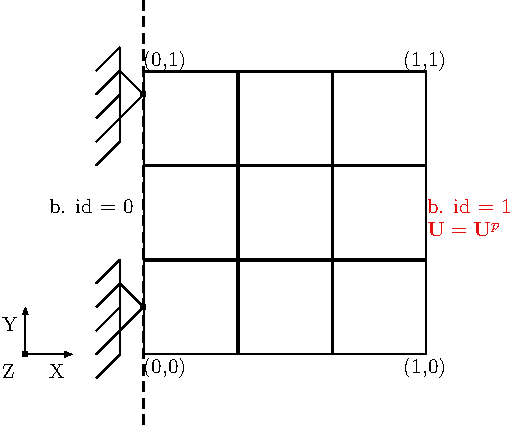
\includegraphics[width=0.95\textwidth]{patch_test_grid.pdf}
\caption{Uniform grid}
\label{fig:1.1.1}
\end{subfigure}
\begin{subfigure}{0.4\textwidth}
\centering
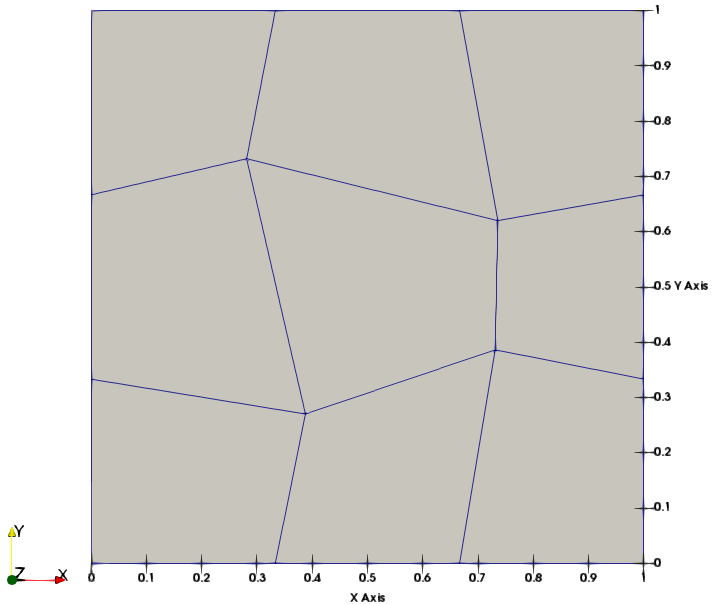
\includegraphics[width=0.7\textwidth]{patch_distort_grid.png}
\caption{Distort grid}
\label{fig:1.1.2}
\end{subfigure}
\caption{Patch test unit cube geometry}
\label{fig:1.1}
\end{figure}

We consider an axisymmetric geometry with unit cube cross section which is discretized into nine elements, cf. Figure \eqref{fig:1.1.1}. To check for the discretization error in the numerical solution using a selected finite element, we also have a distorted grid with the grid points in the interior of mesh distorted in a random way, cf. Figure \eqref{fig:1.1.2}. The hyperelastic Neo-Hookean material model as given in Equation \eqref{eq:1.2} was considered for the patch material. The considered boundary conditions are: homogeneous Dirichlet boundary condition on the boundary consisting the axis of symmetry (boundary id = 0) and inhomogeneous Dirichlet boundary condition (tensile load) on boundary id = 1. The tensile load of $0.1 \ \text{N}$ was applied in a uniformly increasing step of $0.025 \ \text{N}$. Lagrange finite elements with linear and quadratic shape functions were employed for this patch test. One h-adaptive mesh refinement cycle was performed to compare the quality of solution between the coarse mesh and once h-adaptively refined mesh for the distort grid geometry. \par 

\begin{figure}[h]
\centering
\begin{subfigure}[b]{0.35\textwidth}
\centering
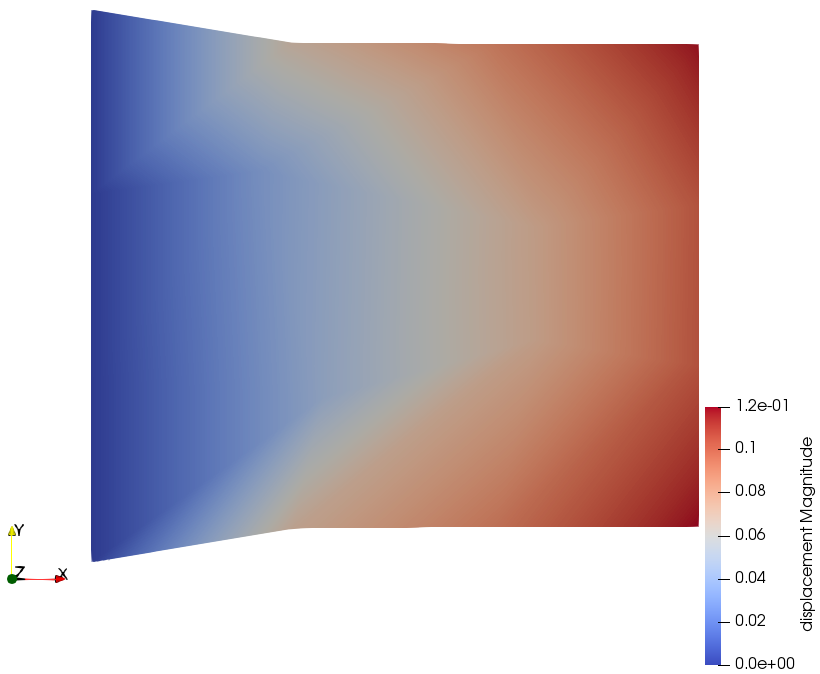
\includegraphics[width=0.9\textwidth]{patch_distort_grid_ref_0.png}
\caption{Linear element: Ref. cycle 0}
\label{fig:1.2.1}
\end{subfigure}
\begin{subfigure}[b]{0.35\textwidth}
\centering
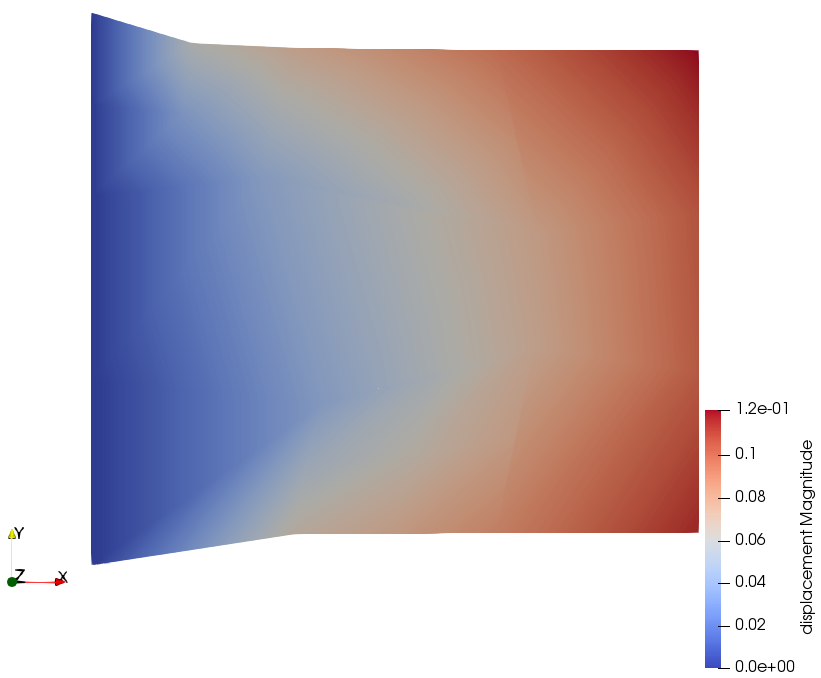
\includegraphics[width=0.9\textwidth]{patch_distort_grid_ref_1.png}
\caption{Linear element: Ref. cycle 1}
\label{fig:1.2.2}
\end{subfigure}
\begin{subfigure}[b]{0.35\textwidth}
\centering
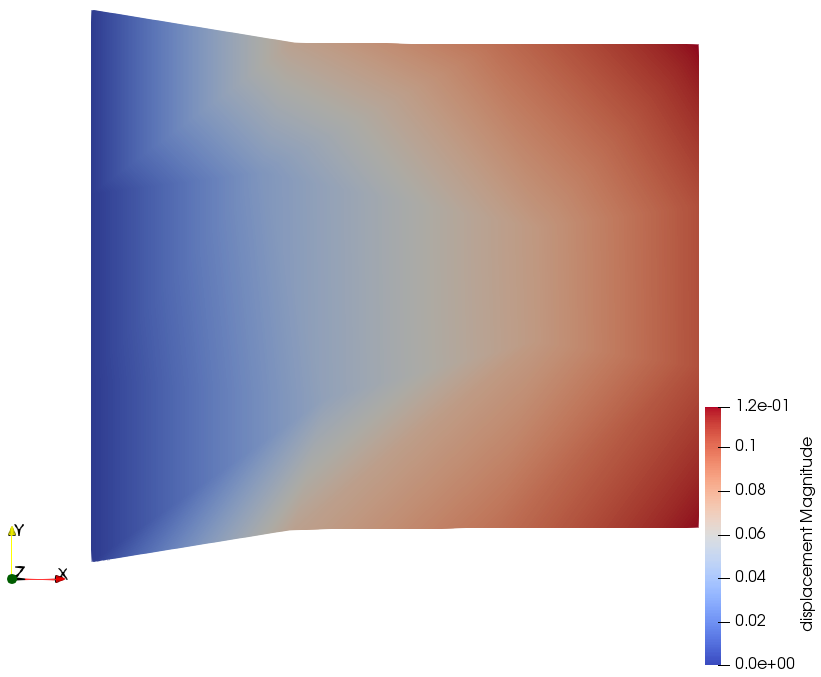
\includegraphics[width=0.9\textwidth]{patch_distort_grid_ref_0_quad.png}
\caption{Quadratic element: Ref. cycle 0}
\label{fig:1.2.3}
\end{subfigure}
\begin{subfigure}[b]{0.35\textwidth}
\centering
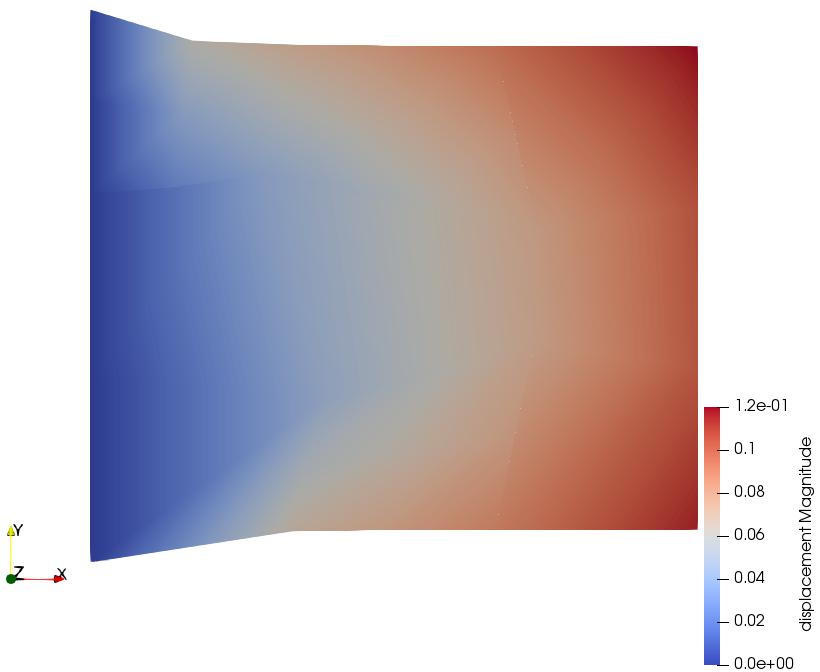
\includegraphics[width=0.9\textwidth]{patch_distort_grid_ref_1_quad.png}
\caption{Quadratic element: Ref. cycle 1}
\label{fig:1.2.4}
\end{subfigure}
\caption{Distort grid displacement at total load}
\label{fig:1.2}
\end{figure}

\begin{figure}[h!]
\centering
\begin{subfigure}[b]{0.35\textwidth}
\centering
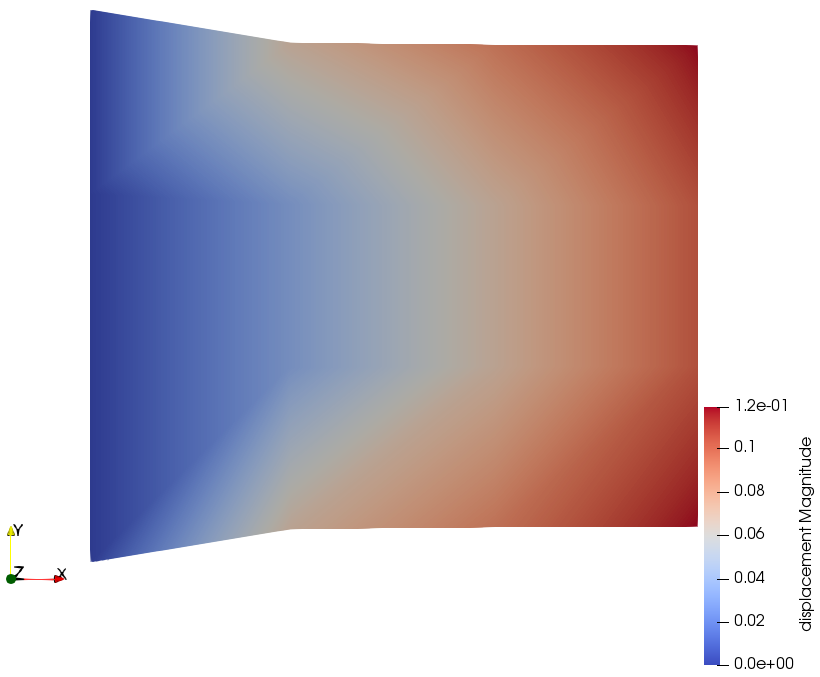
\includegraphics[width=0.9\textwidth]{patch_uniform_grid_ref_0.png}
\caption{Linear element: Ref. cycle 0}
\label{fig:1.3.1}
\end{subfigure}
\begin{subfigure}[b]{0.35\textwidth}
\centering
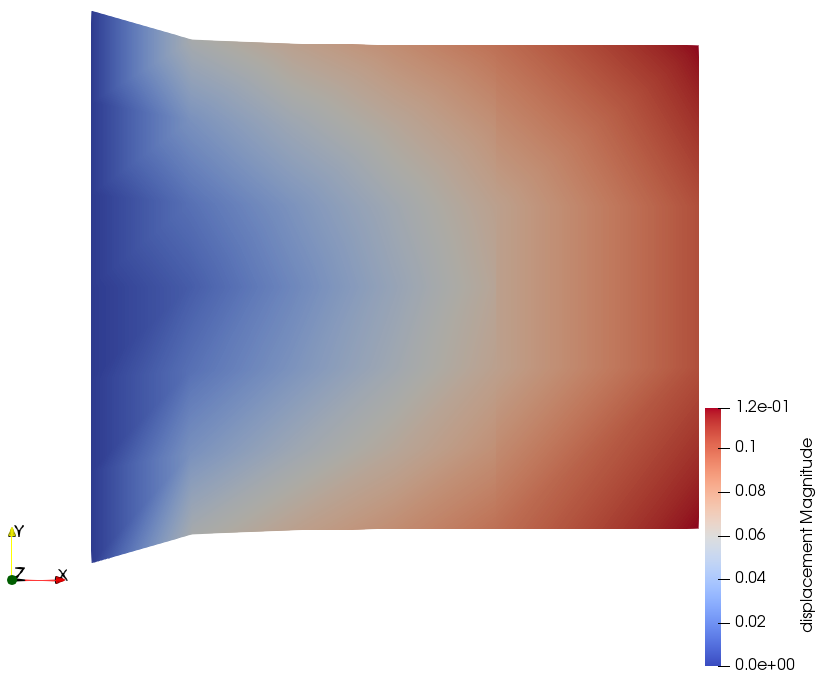
\includegraphics[width=0.9\textwidth]{patch_uniform_grid_ref_1.png}
\caption{Linear element: Ref. cycle 1}
\label{fig:1.3.2}
\end{subfigure}
\begin{subfigure}[b]{0.35\textwidth}
\centering
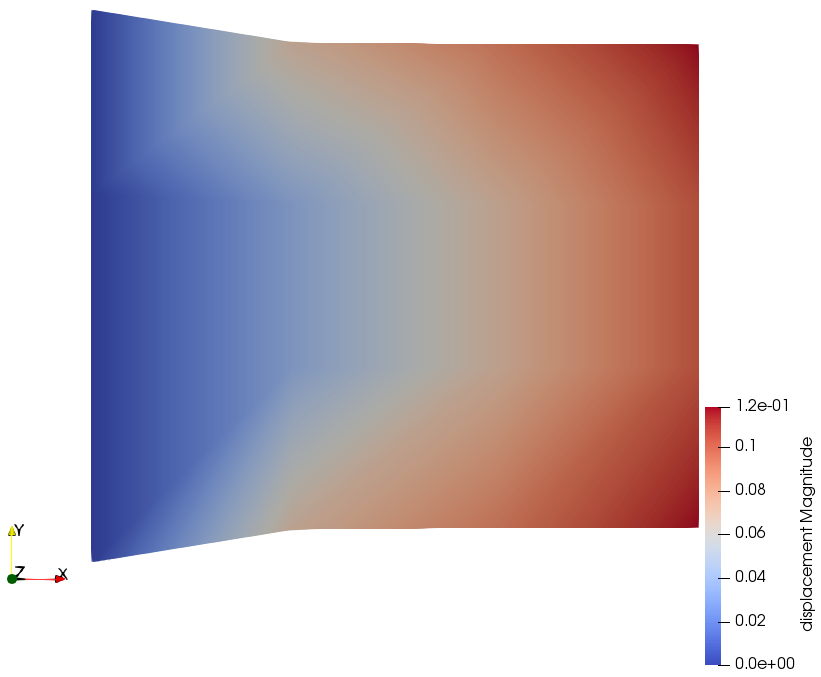
\includegraphics[width=0.9\textwidth]{patch_uniform_grid_ref_0_quad.png}
\caption{Quadratic element: Ref. cycle 0}
\label{fig:1.3.3}
\end{subfigure}
\begin{subfigure}[b]{0.35\textwidth}
\centering
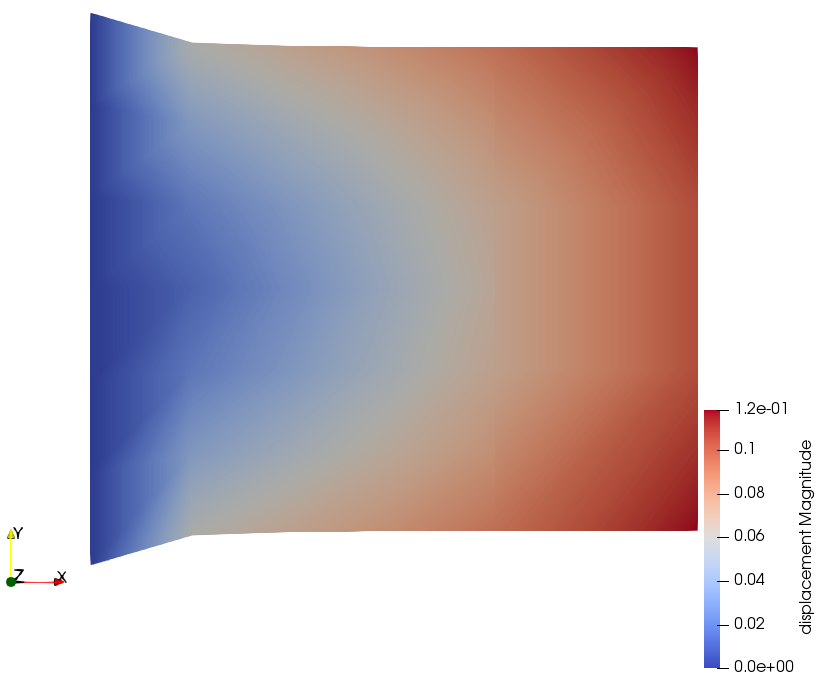
\includegraphics[width=0.9\textwidth]{patch_uniform_grid_ref_1_quad.png}
\caption{Quadratic element: Ref. cycle 1}
\label{fig:1.3.4}
\end{subfigure}
\caption{Uniform grid displacement at total load}
\label{fig:1.3}
\end{figure}

Comparing the results for the final deformed states for the distort mesh Figures \eqref{fig:1.2} and the uniform grid patch Figures \eqref{fig:1.3}, we can confirm that the employed linear (vector-valued) shape functions $(\mathbf{Q}_1 \times \mathbf{Q}_1)$ for the displacement field lead to same results (under given tolerance) as the ones for the quadratic shape functions $(\mathbf{Q}_2 \times \mathbf{Q}_2)$. The deformed states after one refinement cycle for the distort grid are different compared to the uniform grid results, this is due to the different mesh with refined cells which is by the virtue of the adaptive mesh refinement. But the nature of the displacement field is same irrespective of the employed linear or quadratic shape functions. \par 

\subsubsection{Traction boundary condition test}
A unit test to check the traction boundary condition implementation was set up with an axisymmetric beam geometry problem. The considered beam is of length $2 \ \text{m}$ and height $1 \ \text{m}$. The beam is discretized into 8 elements along the length and 4 elements along the height thus giving a total of 32 elements in the coarse mesh. The hyperelastic Neo-Hookean material model as given in Equation \eqref{eq:1.2} was considered for the beam material. The considered boundary conditions are: homogeneous Dirichlet boundary condition on the boundary consisting the axis of symmetry with boundary id = 0 and a uniformly distributed traction load (downward) on the right half of the top boundary of the beam with boundary id = 6, cf. Figure \eqref{fig:1.4}. The considered traction load has a magnitude of $1e^{-3} \frac{\text{N}}{\text{m}}$ distributed uniformly over a length of $1 \ \text{m}$. Employing uniformly increasing load stepping, this traction load was applied in 4 load steps.  The final deformed state for individual refinement cycles are as observed in Figure \eqref{fig:1.5.2} and \eqref{fig:1.5.4}.

\begin{figure}[h]
\centering 
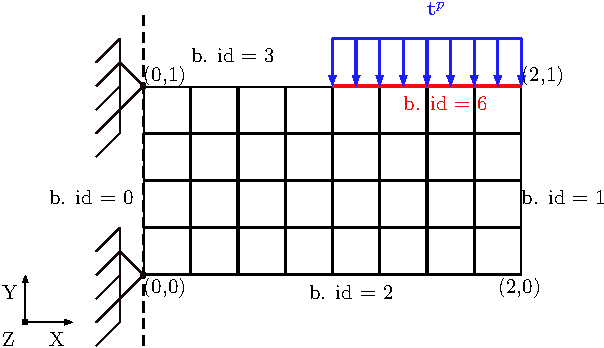
\includegraphics[width=0.4\textwidth]{beam_grid.pdf}
\caption{Beam problem with traction load}
\label{fig:1.4}
\end{figure} 

\begin{figure}[h]
\centering
%\begin{subfigure}[b]{0.45\textwidth}
%\centering
%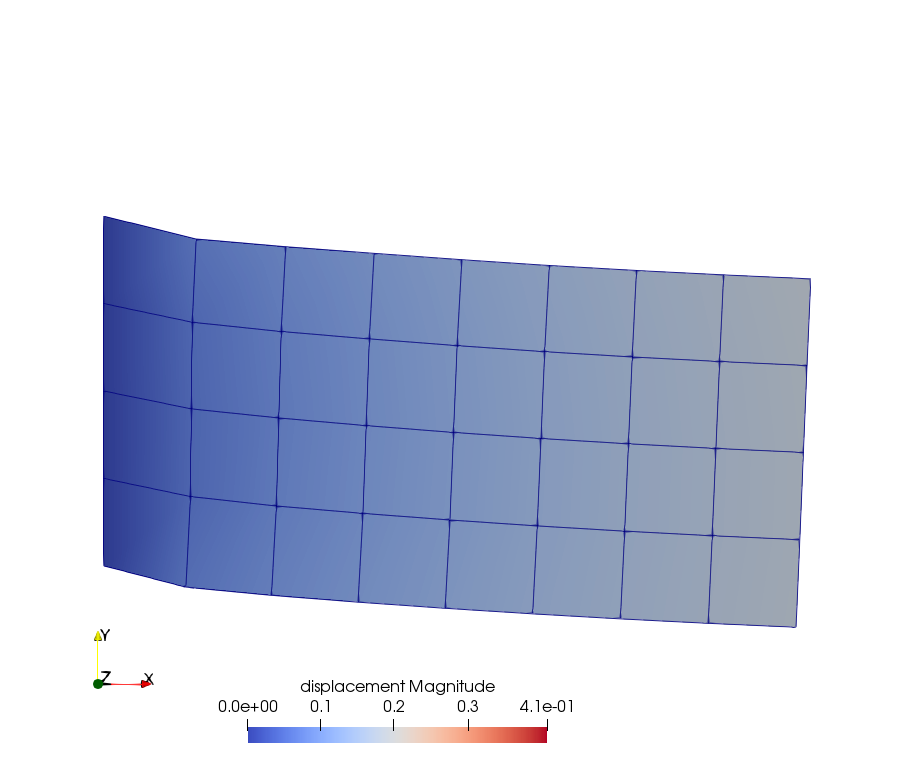
\includegraphics[width=0.9\textwidth]{beam_ref_0_load_half.png}
%\caption{Ref. cycle 0 (half load)}
%\label{fig:1.5.1}
%\end{subfigure}
\begin{subfigure}[b]{0.45\textwidth}
\centering
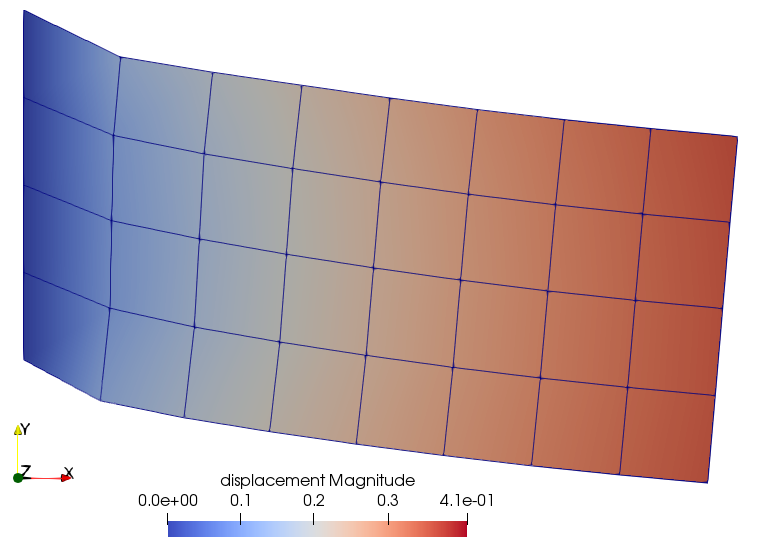
\includegraphics[width=0.9\textwidth]{beam_ref_0_load_full.png}
\caption{Ref. cycle 0}
\label{fig:1.5.2}
\end{subfigure}
%\begin{subfigure}[b]{0.45\textwidth}
%\centering
%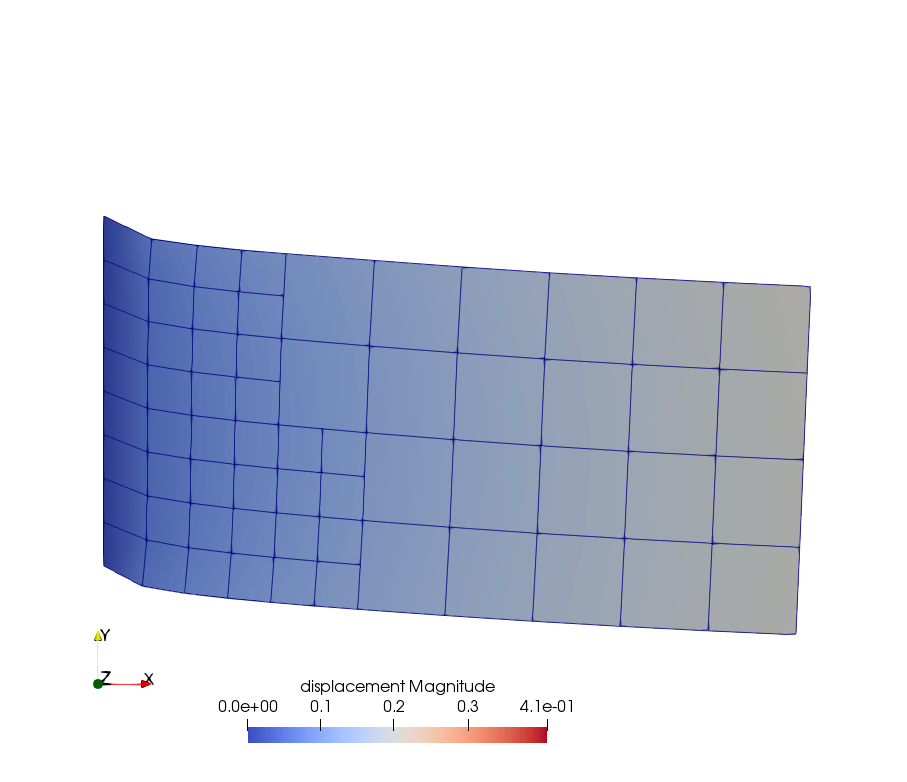
\includegraphics[width=0.9\textwidth]{beam_ref_1_load_half.png}
%\caption{Ref. cycle 1 (half load)}
%\label{fig:1.5.3}
%\end{subfigure}
\begin{subfigure}[b]{0.45\textwidth}
\centering
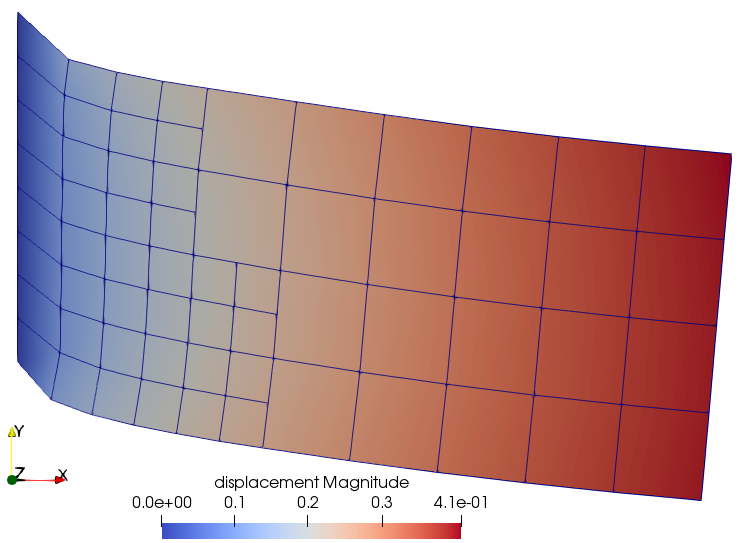
\includegraphics[width=0.9\textwidth]{beam_ref_1_load_full.png}
\caption{Ref. cycle 1}
\label{fig:1.5.4}
\end{subfigure}
\caption{Beam displacement}
\label{fig:1.5}
\end{figure}

\subsubsection{Test for instability behaviour}

Mechanical instability is an important phenomenon in determining the limit loads a structure can handle before becoming unstable. A stable design of the structure exists when the deformations increase as the applied load increases; an unstable design occurs when the deformations increase as the load decreases due to loss of stiffness. Study of such finite elastic deformations of structures helps in understanding the limit loads and prevent sudden buckling / snap-through failures of the structure for applied loads. Referring to Figure \eqref{fig:1.8} commonly known as the load-deflection plot of the equilibrium path, elastic limit point is the critical point after which the structure / material begins to deform largely even for slightly increasing loads. For a load past the critical limit point load $(1)$, the structure undergoes a non-linear buckling which includes a post-buckling instability region. The ``snap-through" occurs in the non-linear instability region and the equilibrium path goes from one stable point $(1)$ to another stable point $(2)$. The non-linear behaviour places the next stable point $(2)$ at the same critical limit load as point $(1)$, but this new load limit at point $(2)$ now corresponds to a new structural shape \cite{Hrinda2010}. The slope of the equilibrium path during the snap-through eventually becomes zero. The slope of this curve is also known as ``tangent stiffness". From a mathematical point of view the determination of instability points is related to the investigation of tangent stiffness with respect to singularities. At the bifurcation point a secondary equilibrium path branches off the primary equilibrium path. Bifurcation point is the limit point at which the structure immediately becomes unstable and buckles. The structure is unable to support any further loads. \par 

\begin{figure}[h]
\centering 
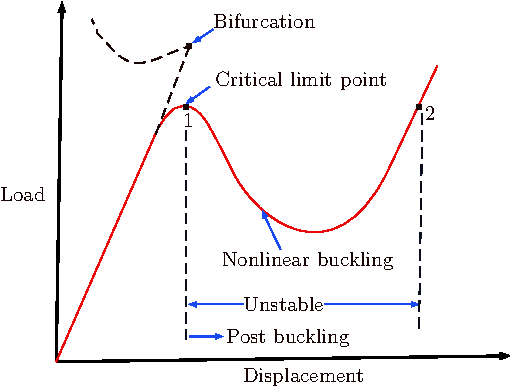
\includegraphics[width=0.6\textwidth]{nonlinear_eq_path.pdf}
\caption{Equilibrium paths for non-linear buckling}
\label{fig:1.8}
\end{figure}

\begin{figure}[ht!]
\centering
\begin{subfigure}[b]{0.6\textwidth}
\centering
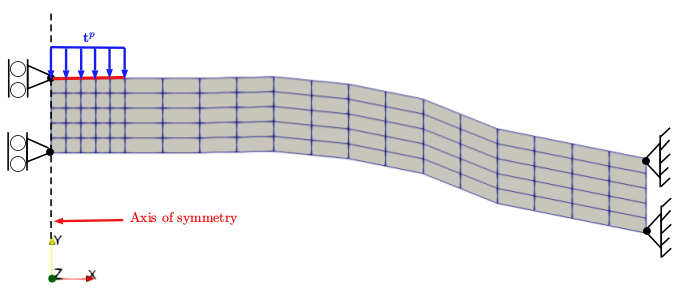
\includegraphics[width=0.95\textwidth]{hooped_beam_grid.png}
\caption{Hooped beam test model}
\label{fig:1.6.1}
\end{subfigure}
\begin{subfigure}[b]{0.39\textwidth}
\centering

\includegraphics[width=0.6\textwidth]{snap_top_mint_box.jpg}
\caption{Mint box illustrating snap through behaviour}
\label{fig:1.6.2}
\end{subfigure}
\caption{Mechanical instability test model 1}
\label{fig:1.6}
\end{figure}

For the stability analysis two test models were implemented as seen in Figure \eqref{fig:1.6.1} and Figure \eqref{fig:1.14}. The first mechanical test model was inspired by a commonly occurring tin mint box with round top, Figure \eqref{fig:1.6.2}, that snaps through to open the box. The cap of this box undergoes a sudden large deformation for an applied point load at the middle point of the round cap. This instability mode is a desired deformation to open the box. On application of equal loads on the opposite ends of the cap, the cap snaps back to the original shape/ form to close the box. To simulate such a sudden snap through behaviour using robust non-linear solvers we developed the axisymmetric hooped beam test model as observed in Figure \eqref{fig:1.6.1}. The out-of-plane displacement of the beam end is fixed by considering pin support (homogeneous D.B.C.) and the edge lying on the axis of symmetry has a sliding contact constraint ($u_x = 0, u_y \neq 0$). A uniformly distributed traction load acts on the top surface of beam as shown in the model. \par 

\begin{figure}[ht!]
\centering
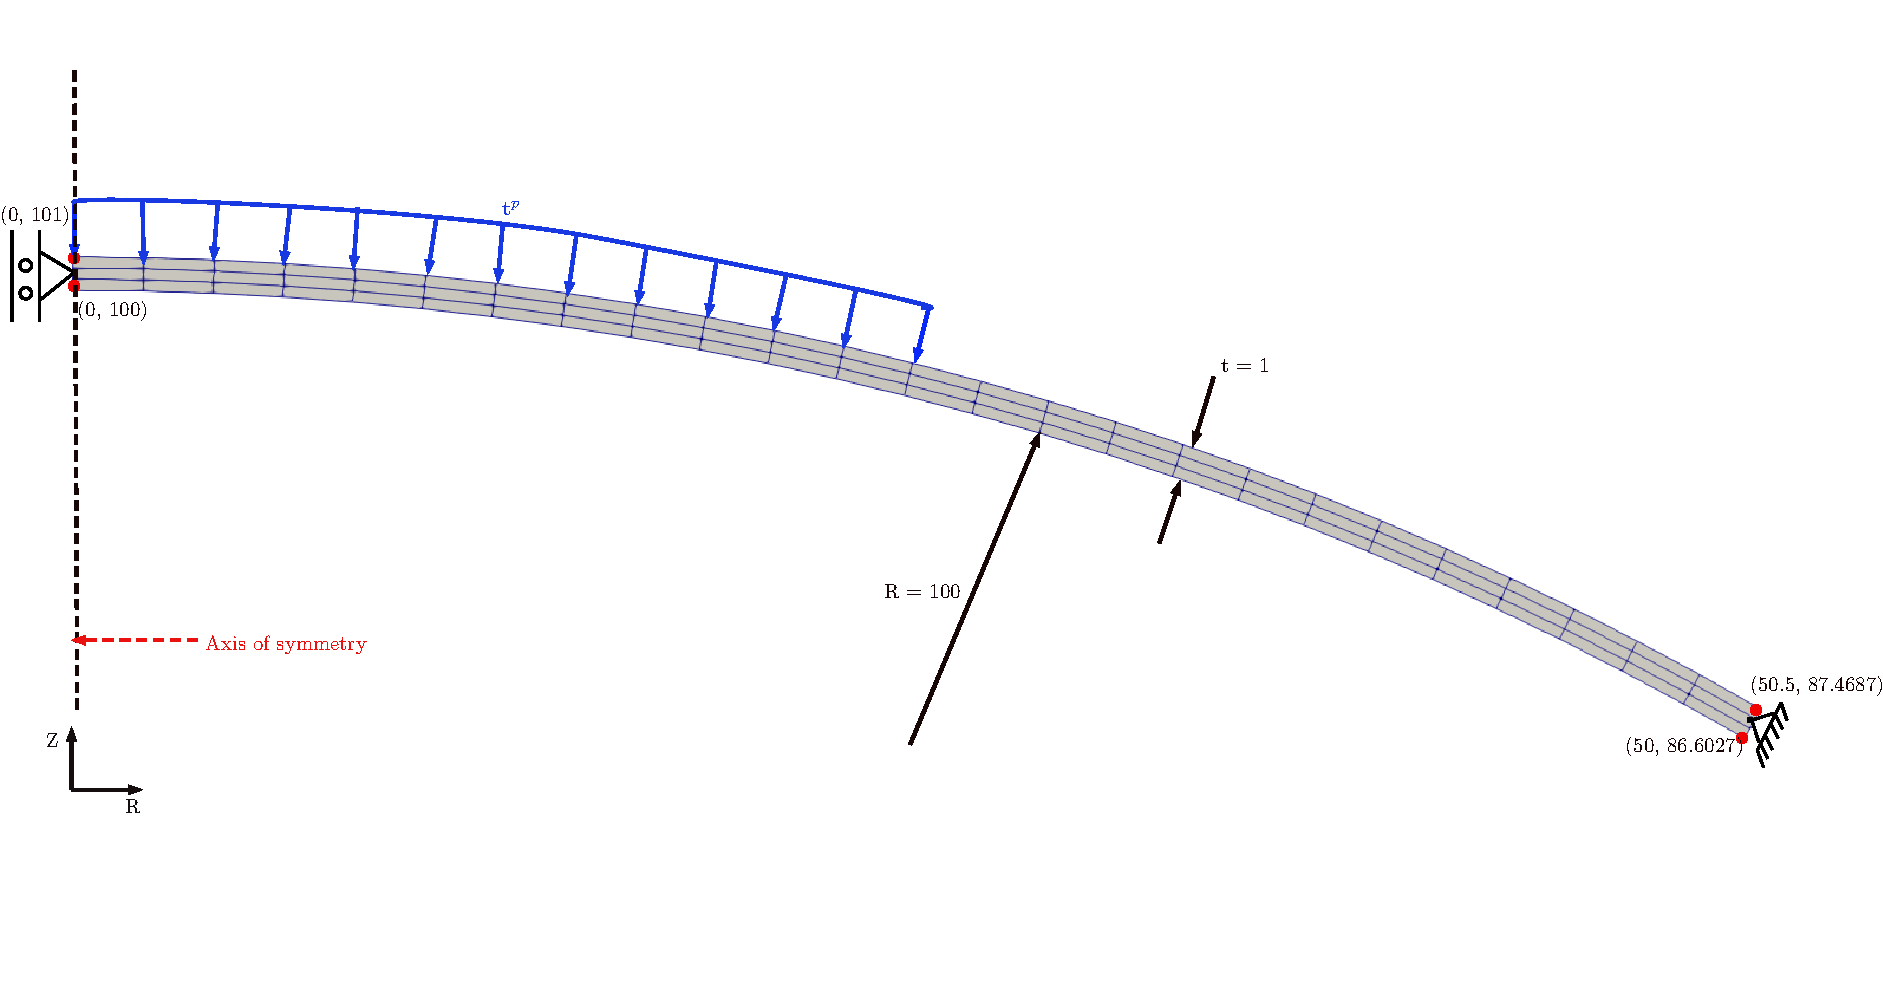
\includegraphics[width=0.7\textwidth]{crisfield_beam.pdf}
\caption{Crisfield beam test model}
\label{fig:1.14}
\end{figure}

The second test model to perform stability analysis of structures is the Crisfield beam, cf. Figure \eqref{fig:1.14}, which is used as a standard benchmark test model to study instability modes \cite[see][page 170]{Wriggers2008} and \cite{Hrinda2010}. \par 

Below results using the Newton-Raphson solution method for the solution of these non-linear test models are presented in Figure \eqref{fig:1.15}. It should be dully noted that the Newton-Raphson solver was not able to capture the instablility modes of deformation even for relatively small load step values ($\approx 1000$ load steps). As pointed out in the literature for the Newton-Raphson solver, it is suspected that the solver jumps from one stable point on the load-displacement equilibrium path to another stable point avoiding the instable buckling path. Thus, we do not observe any instable modes of deformation and for the given loads the structure deforms giving incorrect results as depicted in Figure \eqref{fig:1.15}.\par

\begin{figure}[ht!]
\centering
\begin{subfigure}[b]{0.49\textwidth}
\centering
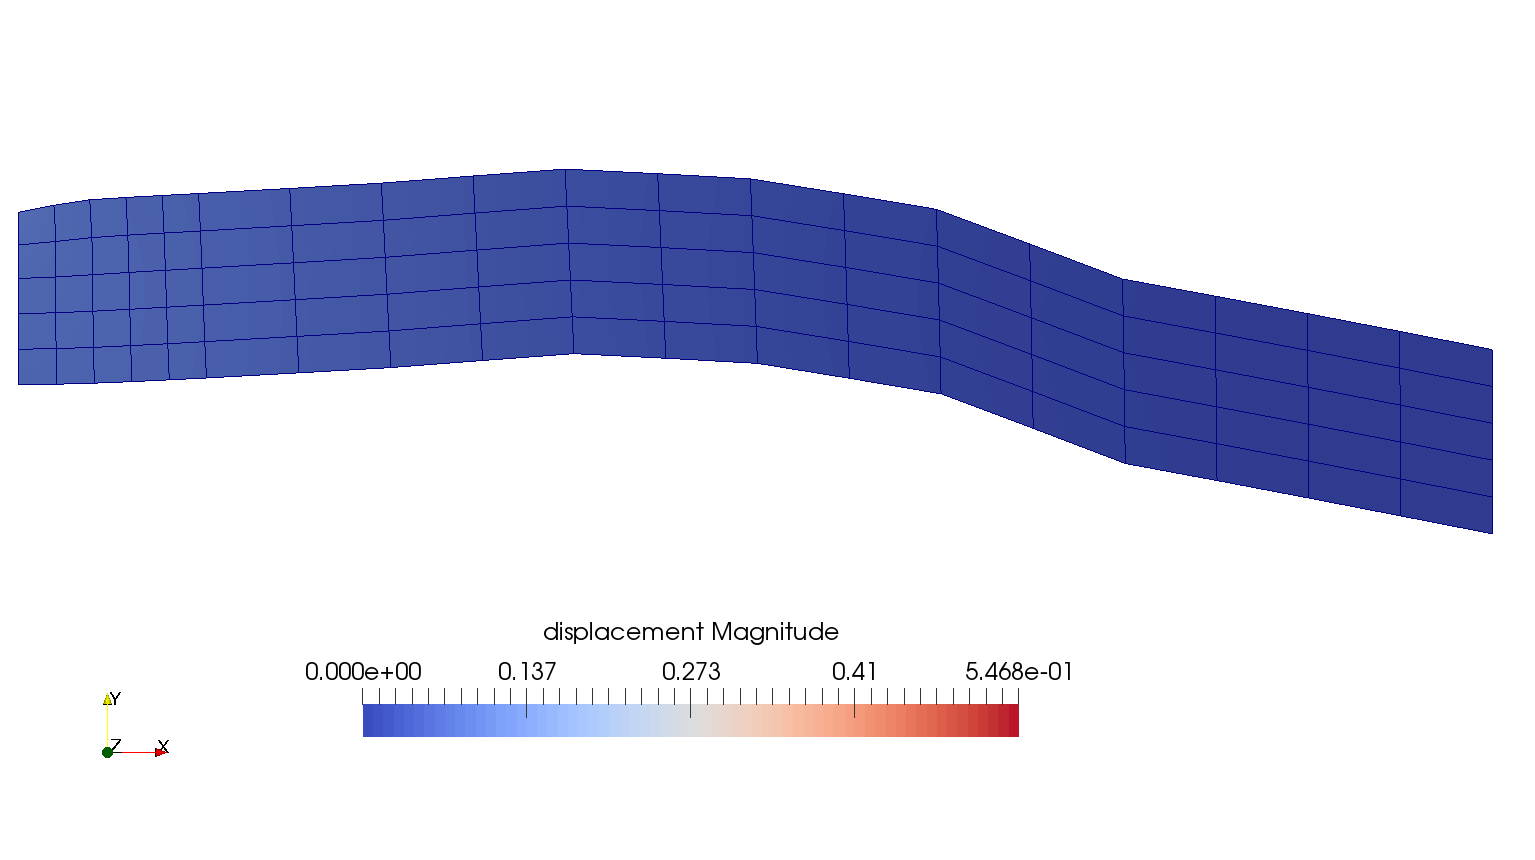
\includegraphics[width=0.95\textwidth]{hooped_ls_4.png}
\caption{Load step 4}
\centering
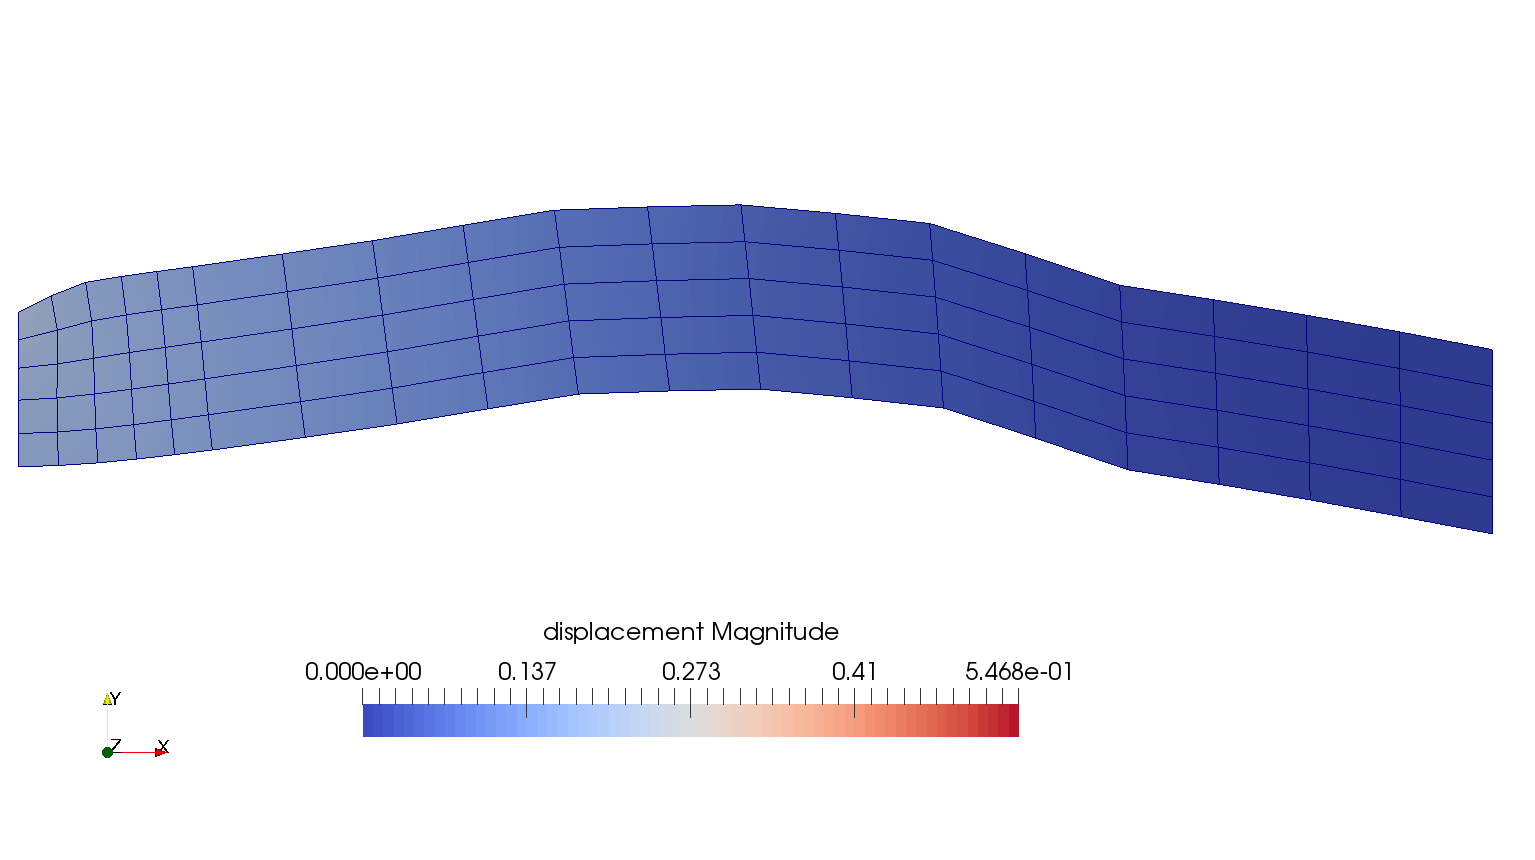
\includegraphics[width=0.95\textwidth]{hooped_ls_9.png}
\caption{Load step 9}
\centering
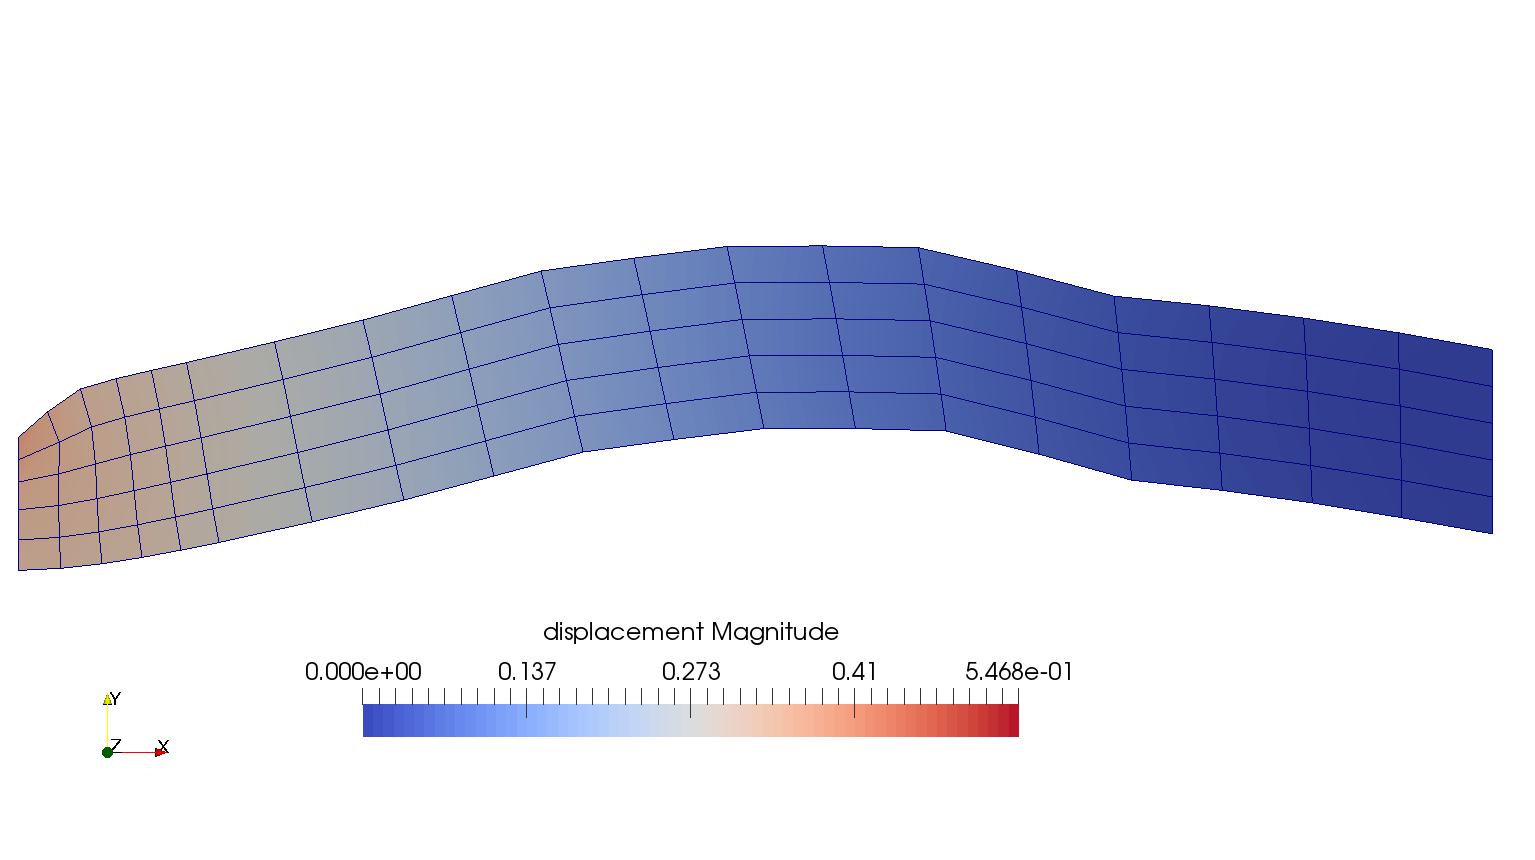
\includegraphics[width=0.95\textwidth]{hooped_ls_14.png}
\caption{Load step 14}
\centering
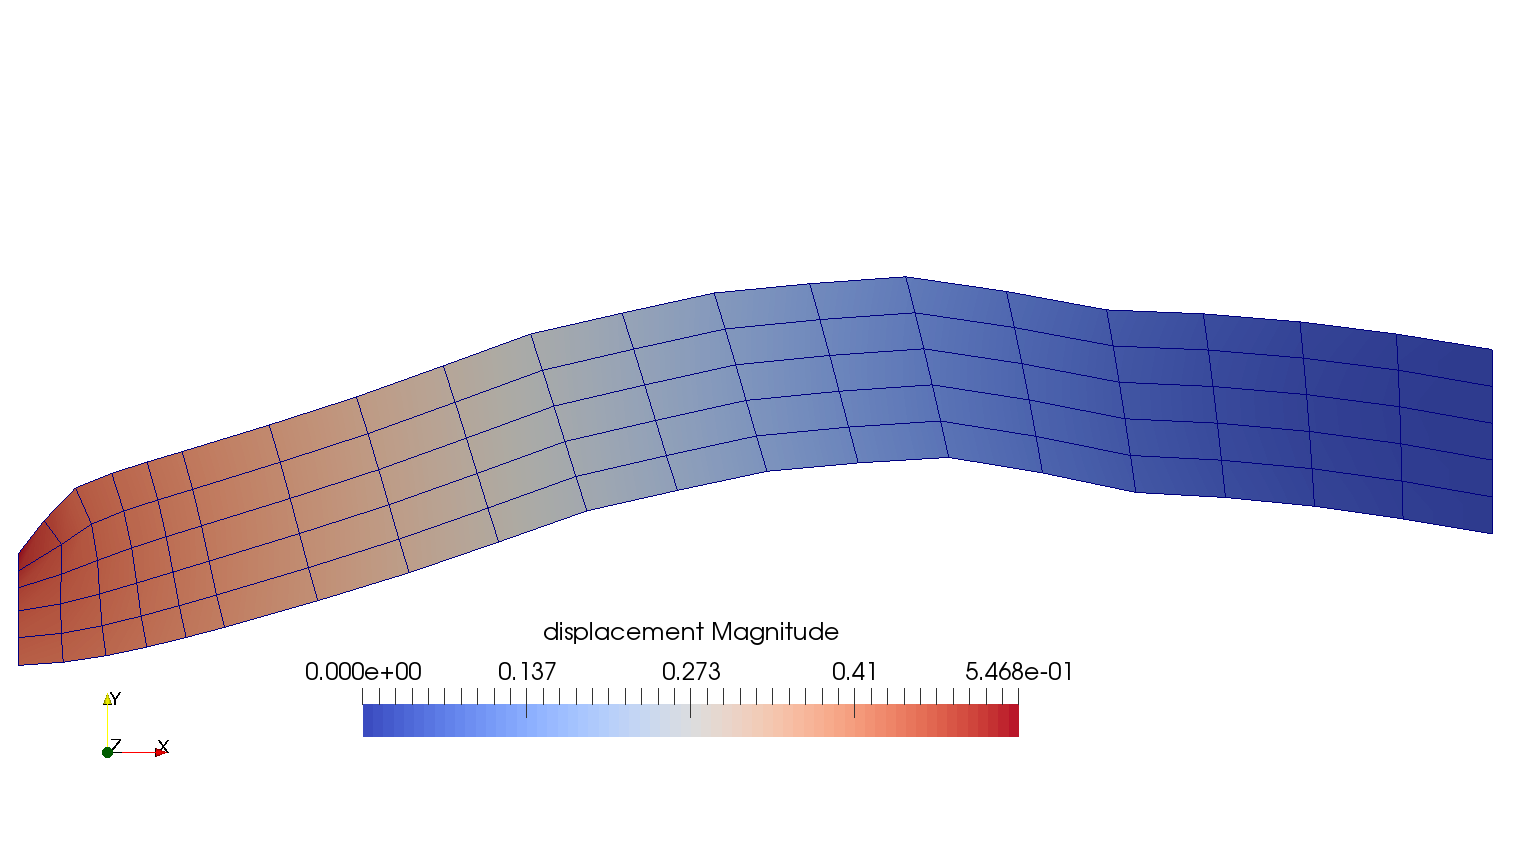
\includegraphics[width=0.95\textwidth]{hooped_ls_19.png}
\caption{Load step 19}
\label{fig:1.15.1}
\end{subfigure}
\begin{subfigure}[b]{0.49\textwidth}
\centering
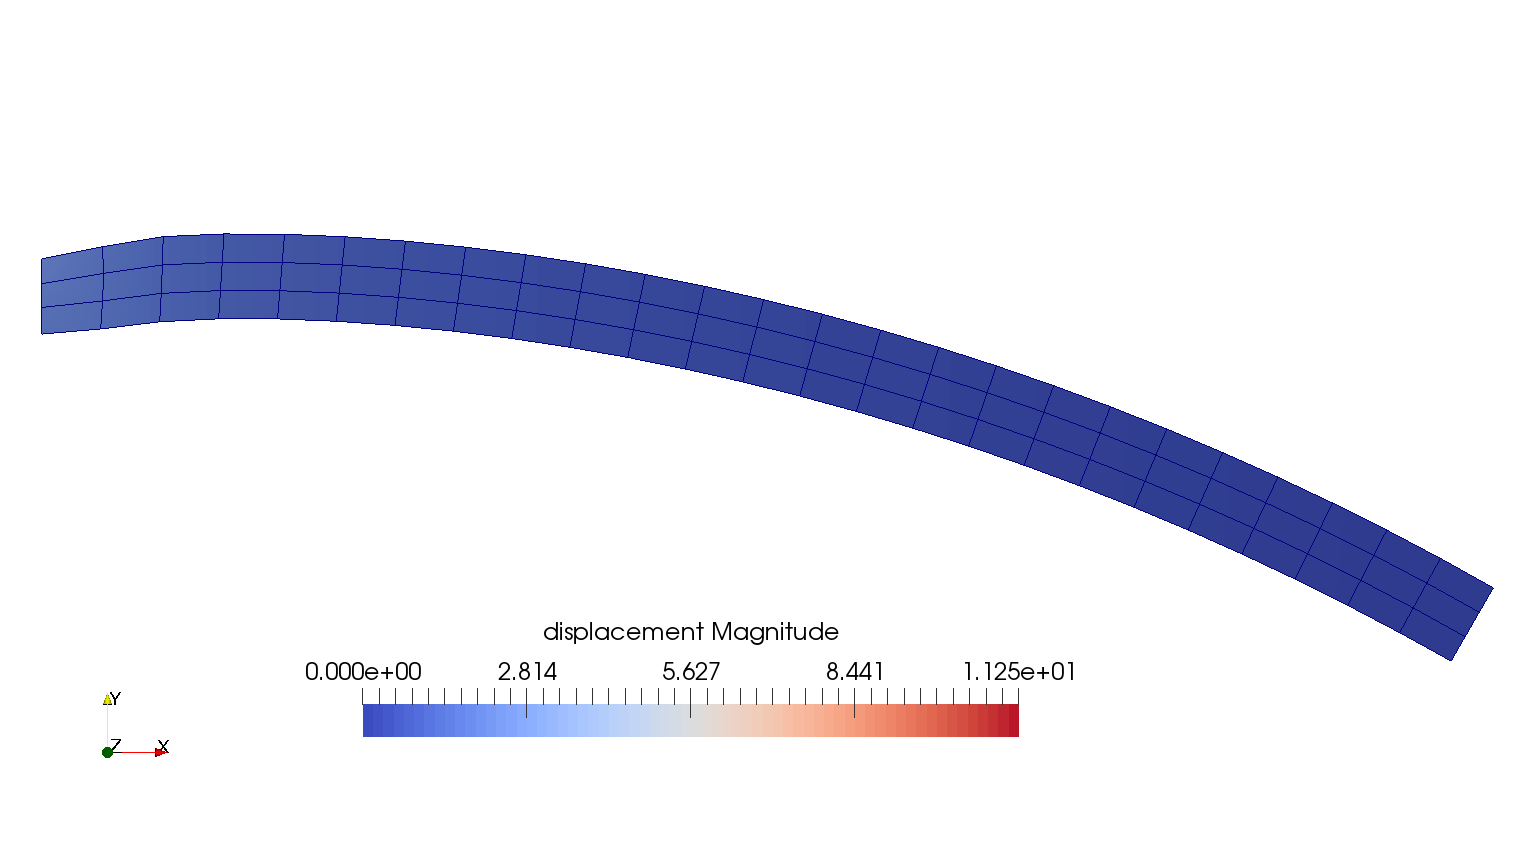
\includegraphics[width=0.95\textwidth]{crisfield_ls_4.png}
\caption{Load step 4}
\centering
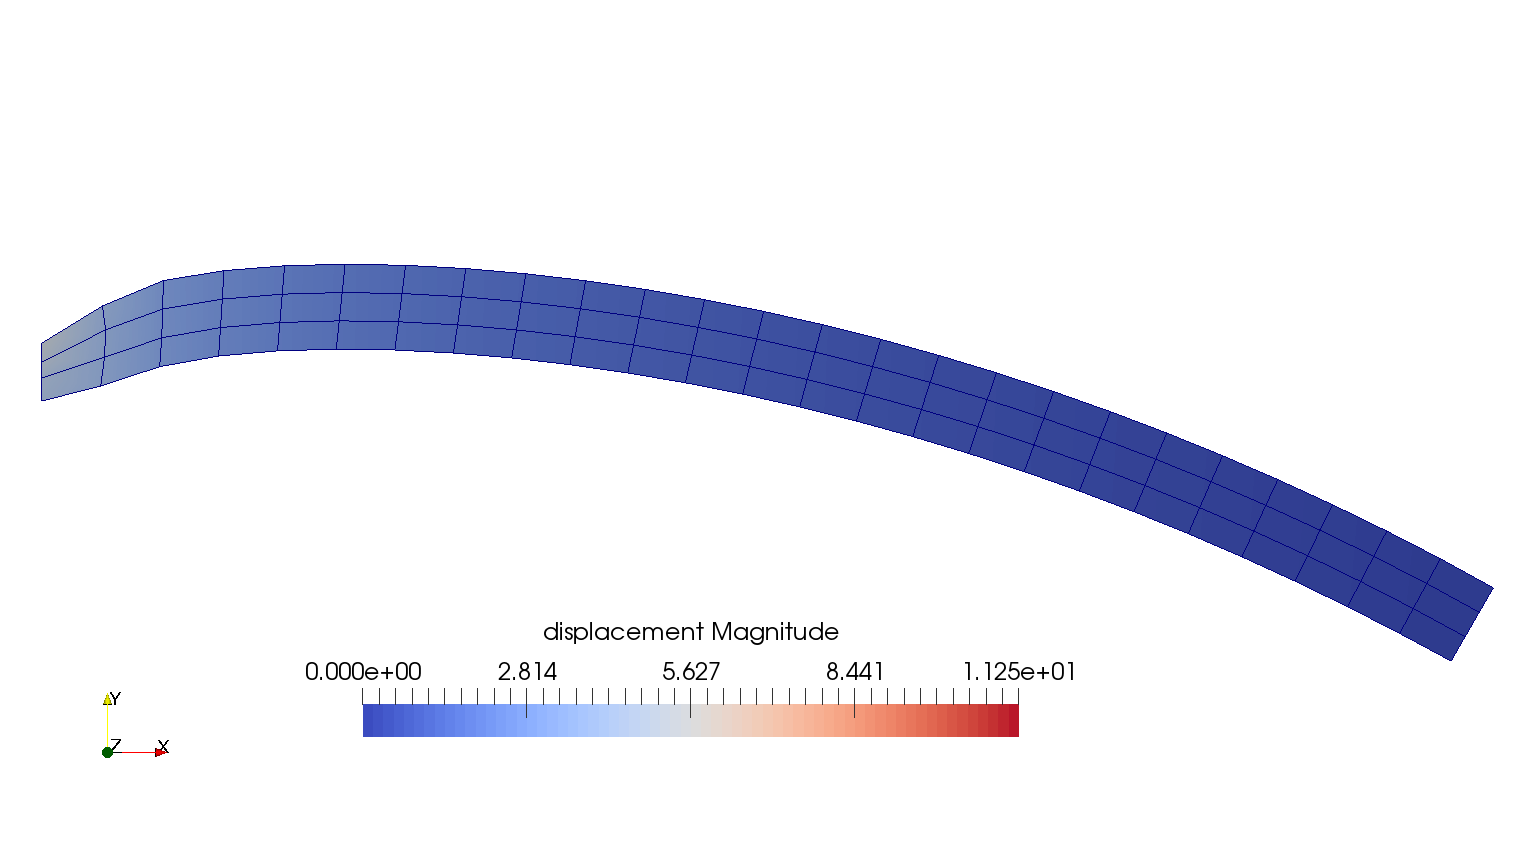
\includegraphics[width=0.95\textwidth]{crisfield_ls_9.png}
\caption{Load step 9}
\centering
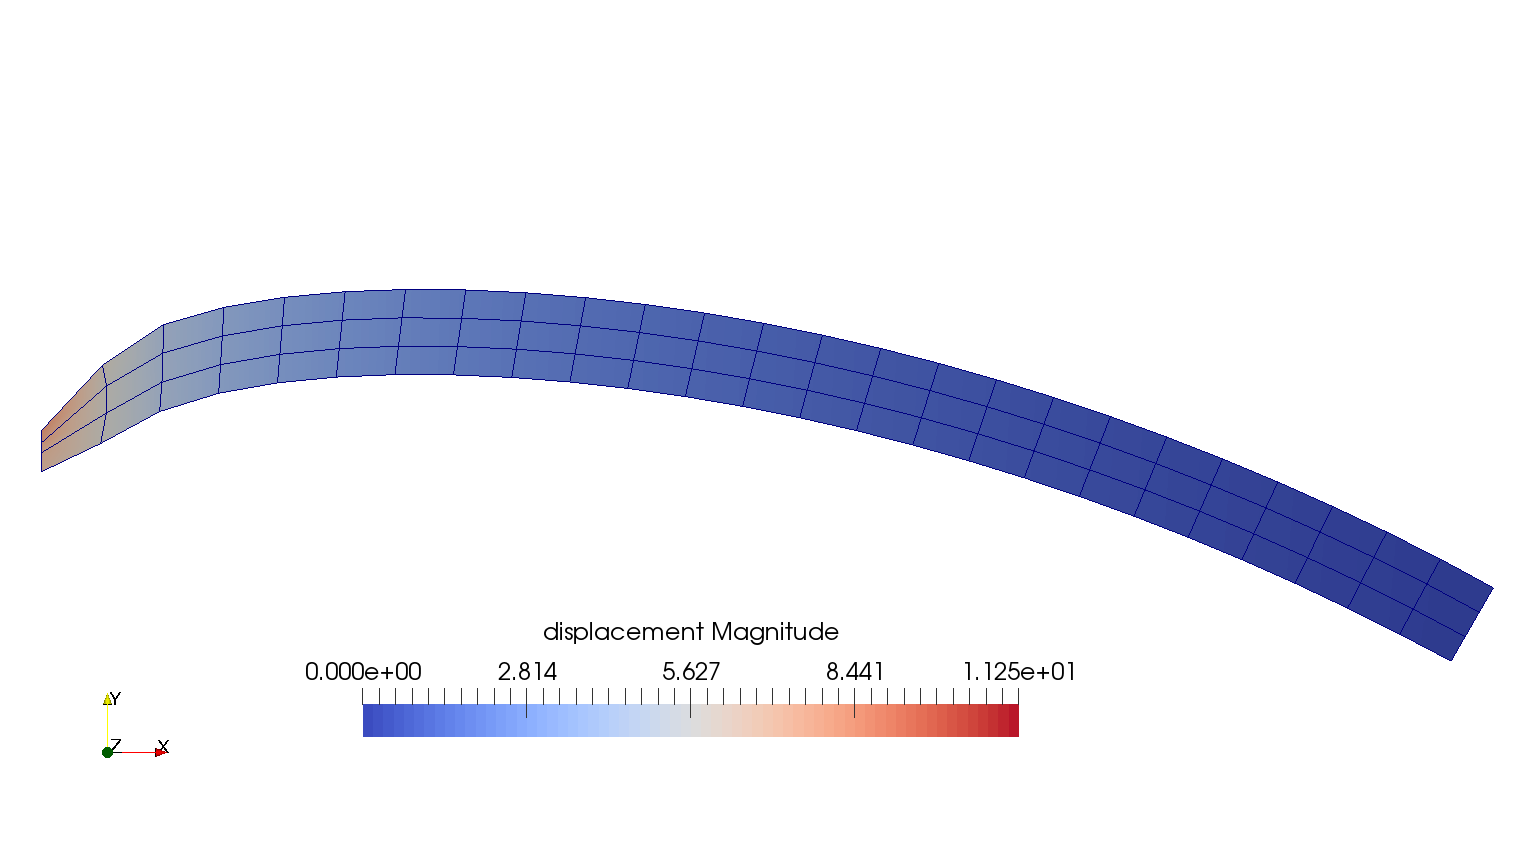
\includegraphics[width=0.95\textwidth]{crisfield_ls_14.png}
\caption{Load step 14}
\centering
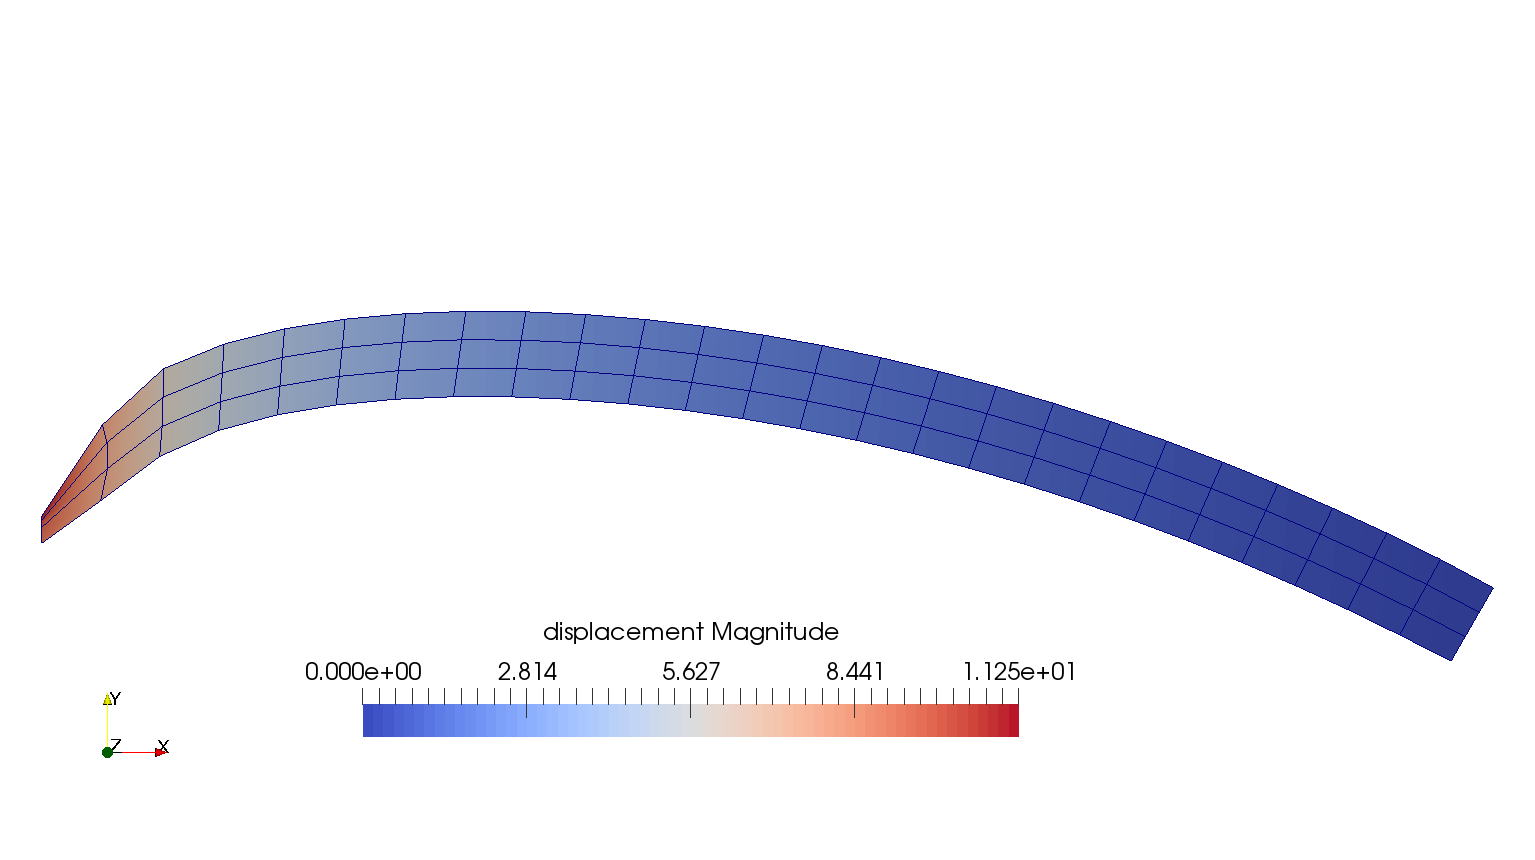
\includegraphics[width=0.95\textwidth]{crisfield_ls_19.png}
\caption{Load step 19}
\label{fig:1.15.2}
\end{subfigure}
\caption{Instability test results}
\label{fig:1.15}
\end{figure}

\subsection{Magneto-elastic torus membrane with free space}
For the geometry of our interest as observed in Figure \eqref{fig:1.7.1}, we now study the elastic finite deformations of the torus magneto-elastic membrane with initial circular cross-section under a quasi-static inflating pressure load. The membrane is modelled as a non-linear elastic material employing the hyperelastic Neo-Hookean material model, cf. Equation \eqref{eq:1.2}. The material parameter values for the magneto-elastic membrane were taken as $\mu = 0.03 \ \text{Pascal}, \ \nu = 0.4$ and the relative magnetic permeability of the membrane as $\mu_r = 6.0$. The surrounding free space (vacuum) through which the magnetic field $\mathbb{H}$ permeates is also modelled as a relatively less stiff elastic material, employing the same Neo-Hookean material model but with different material parameter values of $\mu = 3e^{-5} \ \text{Pascal}$ and $\nu = 0.3$. Employing the total Lagrangian formulation, the inflating pressure load was applied on the undeformed/ reference domain in uniformly increasing load steps as:

\begin{equation}
\mathbf{t}^p = \mathbf{P}\mathbf{N} = \left[ p_0 \mathbf{I} \right] \mathbf{N} = p_0 \mathbf{N},
\end{equation}

\noindent where $\mathbf{P}$ is the $1^{st}$ Piola-Kirchhoff stress, $p_0$ is the inflating pressure load (scalar) and $\mathbf{N}$ is the referential unit inward pointing normal vector for any point on the inner interface of the torus membrane. The inflating pressure load was taken as $p_0 = 1e^{-3} \frac{\text{N}}{\text{m}^2}$. Homogeneous Dirichlet boundary condition was considered for the boundary of the free space domain.\par 

\begin{figure}[h]
\centering 
\begin{subfigure}[b]{0.6\textwidth}
\centering
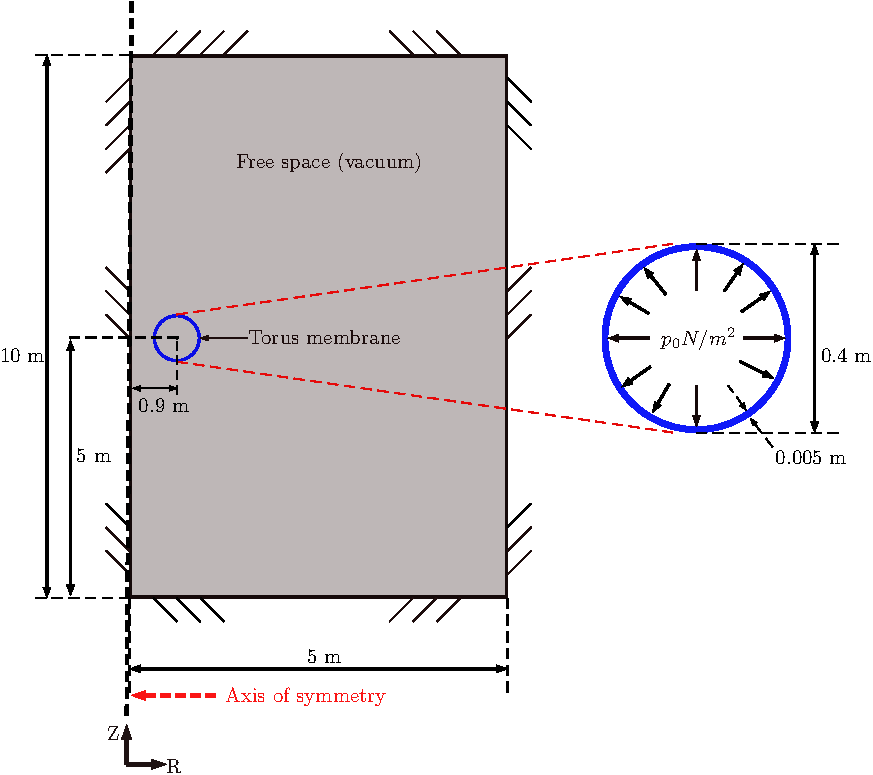
\includegraphics[width=0.9\textwidth]{torus_membrane_grid.pdf}
\caption{\scriptsize{Problem description}}
\label{fig:1.7.1}
\end{subfigure}
\begin{subfigure}[b]{0.39\textwidth}
\centering
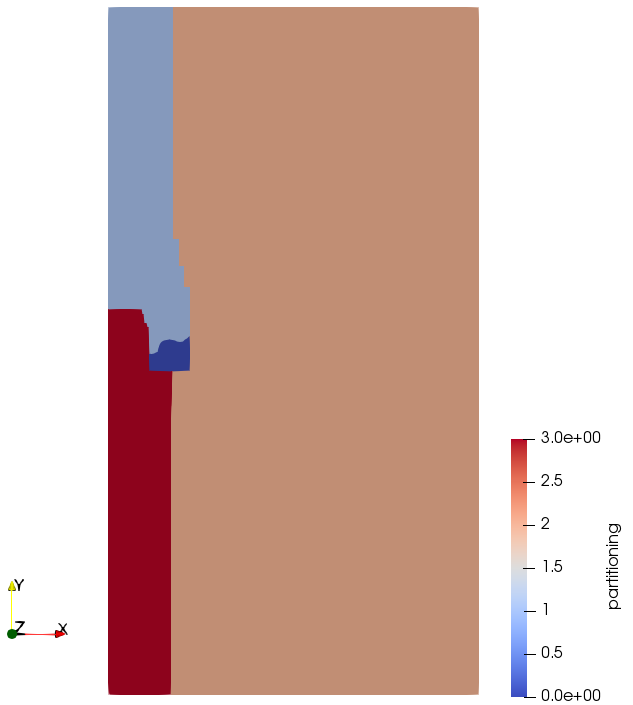
\includegraphics[width=0.9\textwidth]{torus_grid_domain_decomp.png}
\caption{\scriptsize{Domain decomposition for 4 MPI processes}}
\label{fig:1.7.2}
\end{subfigure}
\caption{Magneto-elastic membrane under uniform inflating pressure load}
\label{fig:1.7}
\end{figure} 

The result of the above described uniformly inflating membrane problem is as observed in the Figure \eqref{fig:1.9}. Due to the applied mechanical load, here quasi-static uniform inflating pressure load on inner interface of the membrane, large deformations are observed in the membrane and the surrounding elements of the free space. The deformations in the membrane are relatively large on the right half of the circular cross section when compared to the left half. This is due to the dependence of the deformation gradient $\mathbf{F}$ (component $F_{33}$) on the radial distance of the respective point on the membrane from the axis of symmetry, cf. Equation \eqref{eq:1.26}. Thus for any point on the torus membrane, with increasing radial distance the resulting displacements increase. For the considered free space parameters of $\mu = 3e^{-5} \ \text{Pascal}$ and $\nu = 0.3$, one can observe that the free space material acts relatively less stiff and thus allows for a free inflation of the membrane without any considerable reactive force/ pressure load exerted by the free space material on the inflating membrane. The degree of deformations of the free space elements for increasing pressure load can be observed in Figure \eqref{fig:1.10}. \par 

Element-wise volume averaged Cauchy stress $\bm{\sigma}$ components (radial component $\sigma_{rr}$ and theta component $\sigma_{\theta \theta}$) were also computed to have an understanding of the resulting engineering stress in the torus membrane. The element-wise volume averaged stress was computed as:
\begin{equation}
\left\langle \bm{\sigma} \right\rangle_e := \dfrac{\int\limits_{\Omega_{e}} \bm{\sigma} \mathrm{d}V_e}{\int\limits_{\Omega_{e}} \mathrm{d}V_e} = \dfrac{\sum\limits_{q} \bm{\sigma}(q) * J(q) * w(q)}{\sum\limits_{q} J(q) * w(q)}.
\end{equation}  
The resulting element averaged Cauchy stress components can be observed in Figure \eqref{fig:1.11}. 

\begin{figure}[h]
\centering
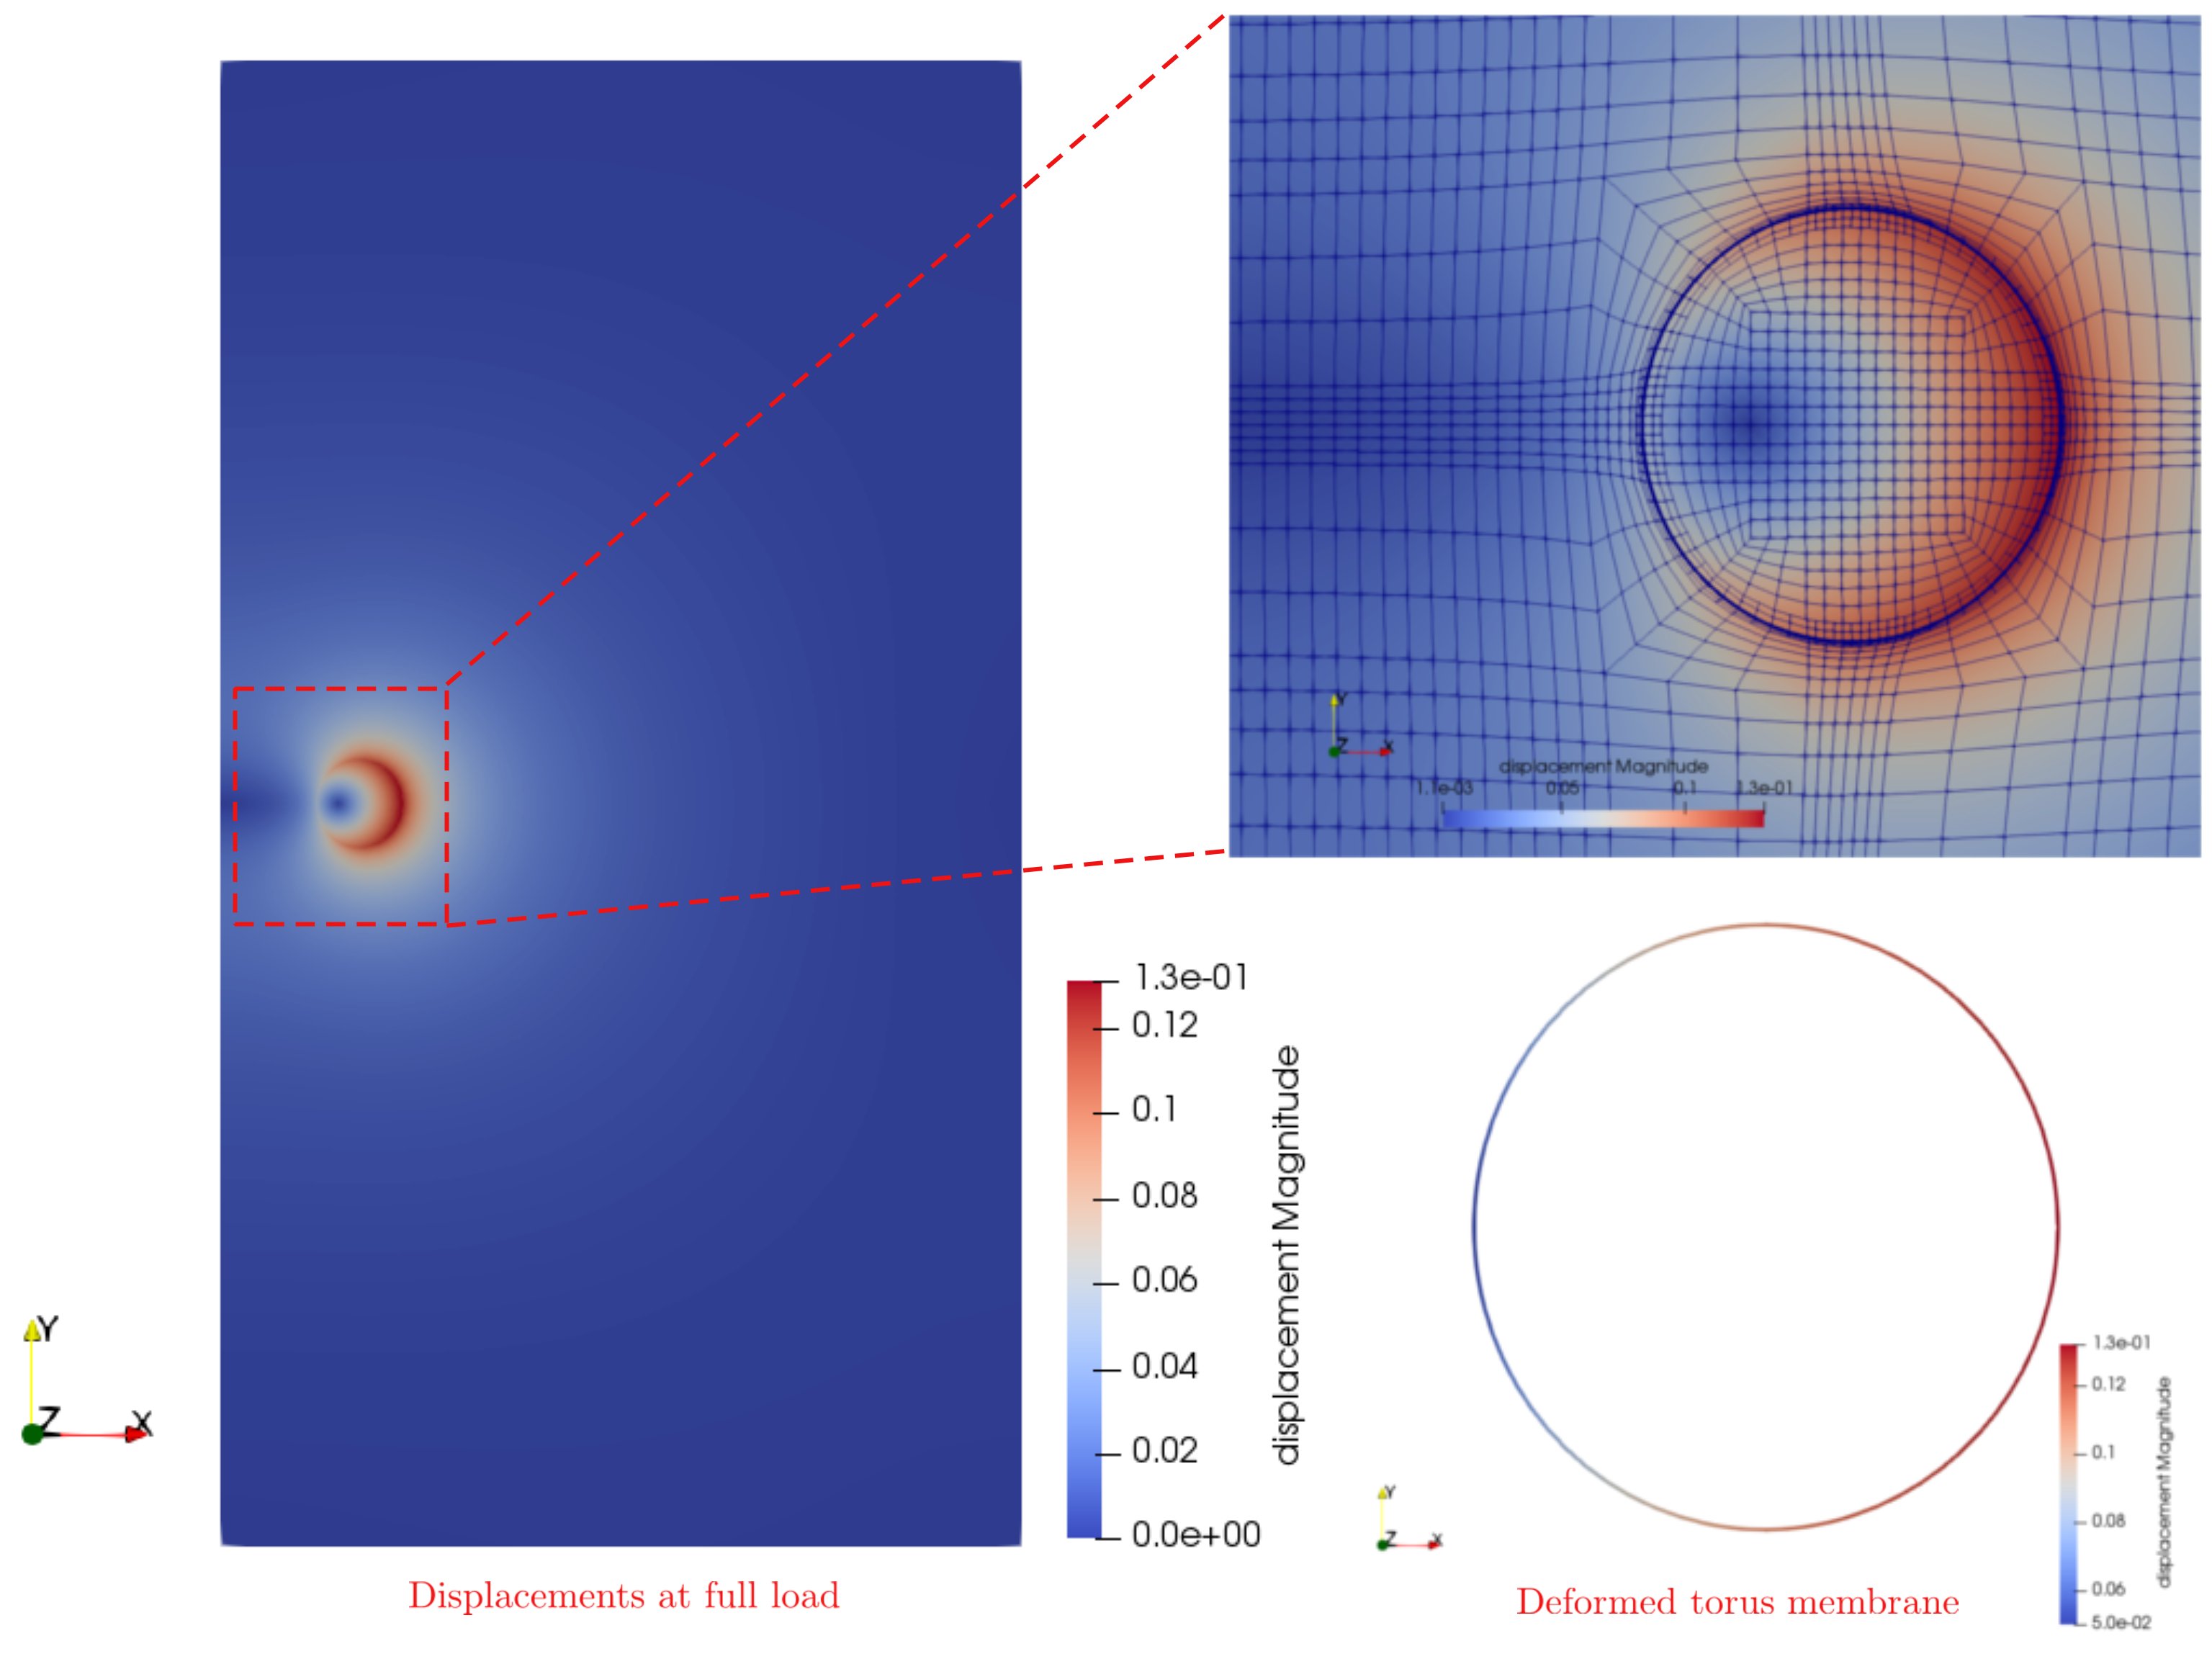
\includegraphics[width=0.7\textwidth]{torus_disp_mue_1000_2.png}
\caption{Deformations at full load}
\label{fig:1.9}
\end{figure}

\begin{figure}[h]
\centering 
\begin{subfigure}[b]{0.32\textwidth}
\centering
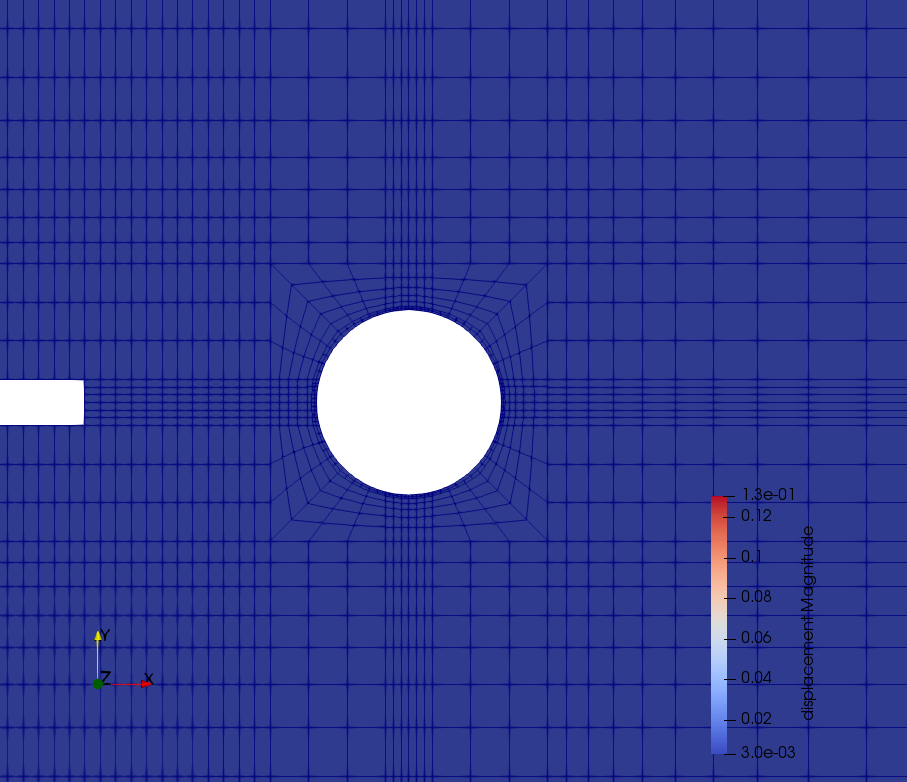
\includegraphics[width=0.95\textwidth]{free_space_disp_0.png}
\caption{Load step 0 (no load)}
\label{fig:1.10.1}
\end{subfigure}
\begin{subfigure}[b]{0.32\textwidth}
\centering
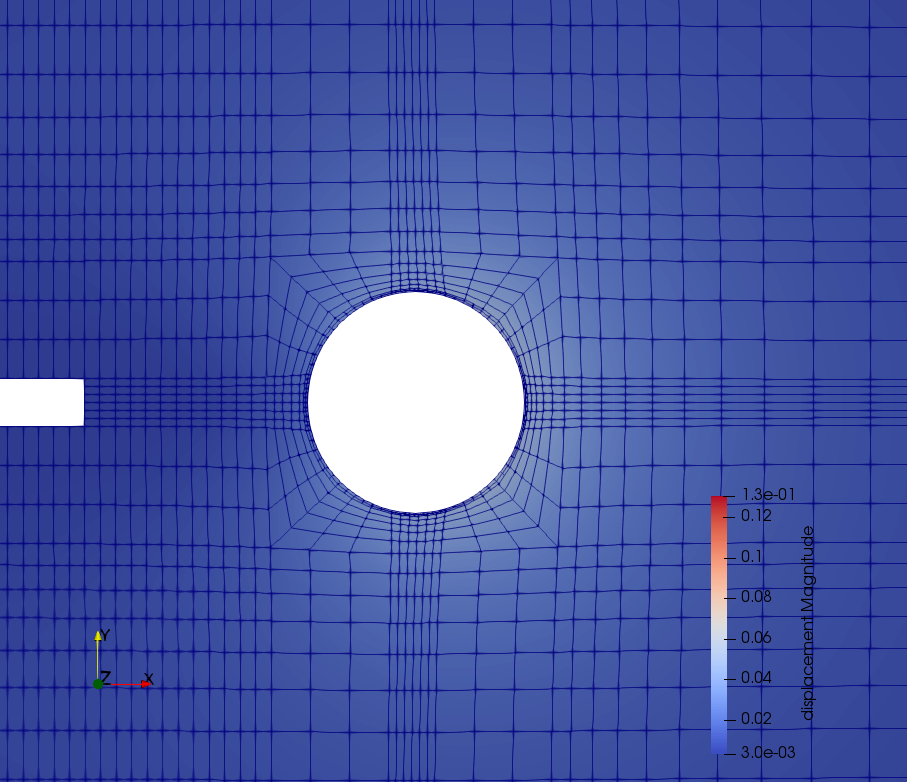
\includegraphics[width=0.95\textwidth]{free_space_disp_9.png}
\caption{Load step 9 (Half load)}
\label{fig:1.10.2}
\end{subfigure}
\begin{subfigure}[b]{0.32\textwidth}
\centering
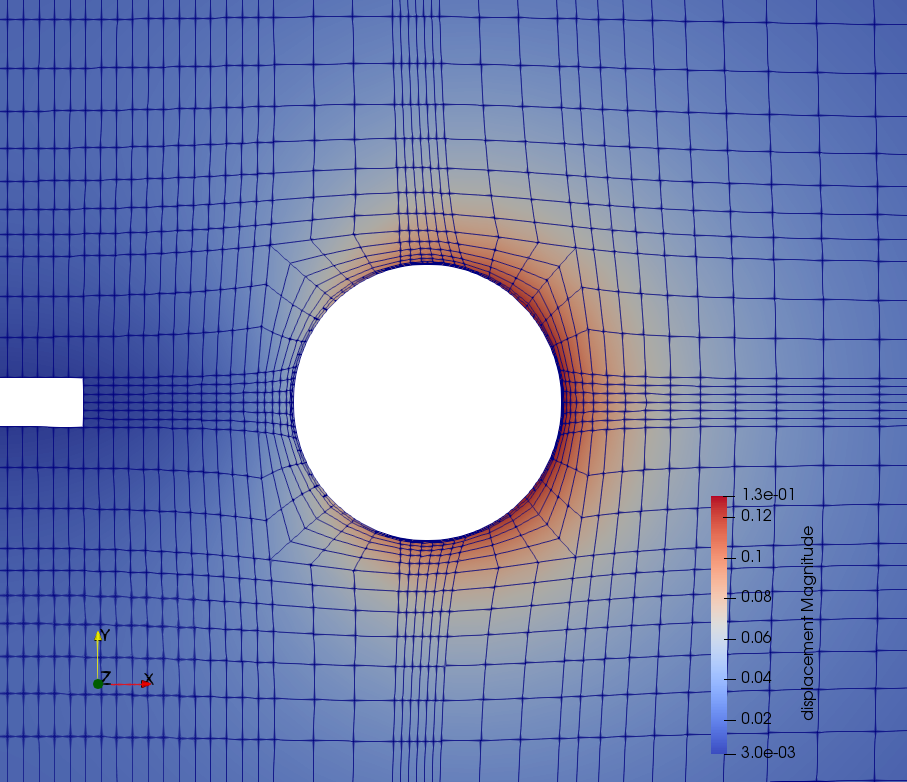
\includegraphics[width=0.95\textwidth]{free_space_disp_19.png}
\caption{Load step 19 (Full load)}
\label{fig:1.10.3}
\end{subfigure}
\caption{Free space (vacuum) deformations}
\label{fig:1.10}
\end{figure}

\begin{figure}[ht!]
\centering 
\begin{subfigure}[b]{0.49\textwidth}
\centering
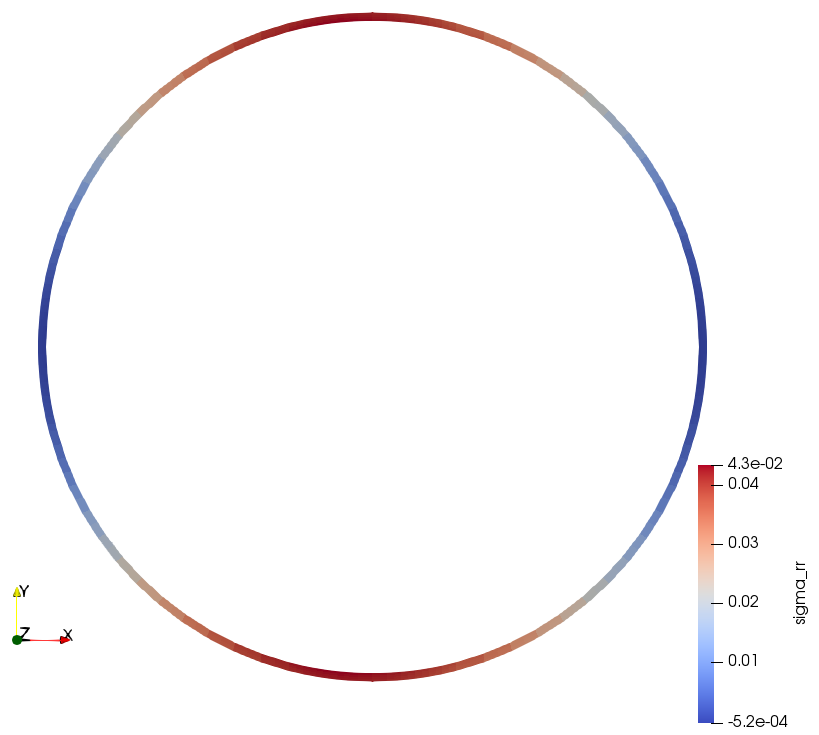
\includegraphics[width=0.9\textwidth]{torus_avg_sigma_rr_mue_1000.png}
\caption{$\sigma_{rr}$}
\label{fig:1.11.1}
\end{subfigure}
\begin{subfigure}[b]{0.49\textwidth}
\centering
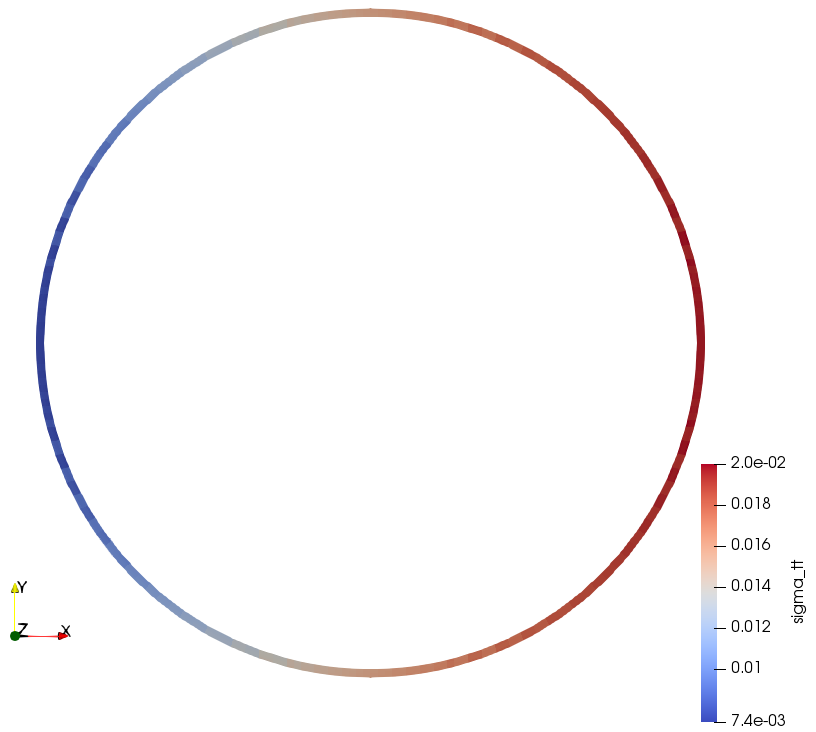
\includegraphics[width=0.9\textwidth]{torus_avg_sigma_theta_mue_1000.png}
\caption{$\sigma_{\theta \theta}$}
\label{fig:1.11.2}
\end{subfigure}
\caption{Element averaged Cauchy stress components for torus membrane}
\label{fig:1.11}
\end{figure} 

\subsection{Parametric study of free space parameter $\mu$}
A parametric study of the free space shear modulus $\mu$ was carried out for the finite strain axisymmetric torus elasticity problem. For the given inflating pressure load of $p_0 = 1e^{-3} \frac{\text{N}}{\text{m}^2}$, torus membrane parameters $\mu = 0.03 \ \text{Pascal}, \ \nu = 0.4$ and the relative permeability as $\mu_r = 6.0$, along with fixed value for the Poisson's ratio of the free space material as $\nu = 0.3$, the free space shear modulus $\mu$ was varied between $\mu_1 = 3e^{-5} \ \text{Pascal}$ and $\mu_2 = 3e^{-4} \ \text{Pascal}$. As expected, with higher value of the free space shear modulus $\mu = 3e^{-4} \ \text{Pascal}$ the free space material acts more stiff and we observe the effect of this increased stiffness on the deformation of the torus membrane for the same applied pressure load. As observed in Figure \eqref{fig:1.12.2}, the resultant deformed state of the torus membrane for the value of $\mu_2$, the stiffer free space material obstructs the free inflation of the membrane. Thus, we have relatively less deformed membrane when compared to the deformed state for $\mu_1$. The resulting element averaged Cauchy stress components can be observed in Figure \eqref{fig:1.13}. The developed stress due to larger deformations of the membrane for less stiffer free space material is higher than the resulting stress for the more stiffer free space material. \par 

For appropriate modelling of the membrane and free space with considered assumptions, it is necessary that we choose the parameter values for the free space such that we can closely approximate our free space material (which is modelled as a non-linear elastic material) as being a fluid region with negligible stiffness and thus exerting negligible loads on the inflating elastic torus membrane geometry of our interest. For values of $\mu < 3e^{-5} \ \text{Pascal}$, we observed negligible differences in the resulting deformed states and stress, when compared to the results for the value of $\mu = 3e^{-5} \ \text{Pascal}$. Thus, a chosen value of $\mu \approx 3e^{-5} \ \text{Pascal}$ can be considered as appropriate to model the free space. \par 

\begin{figure}[ht!]
\centering 
\begin{subfigure}[b]{0.49\textwidth}
\centering
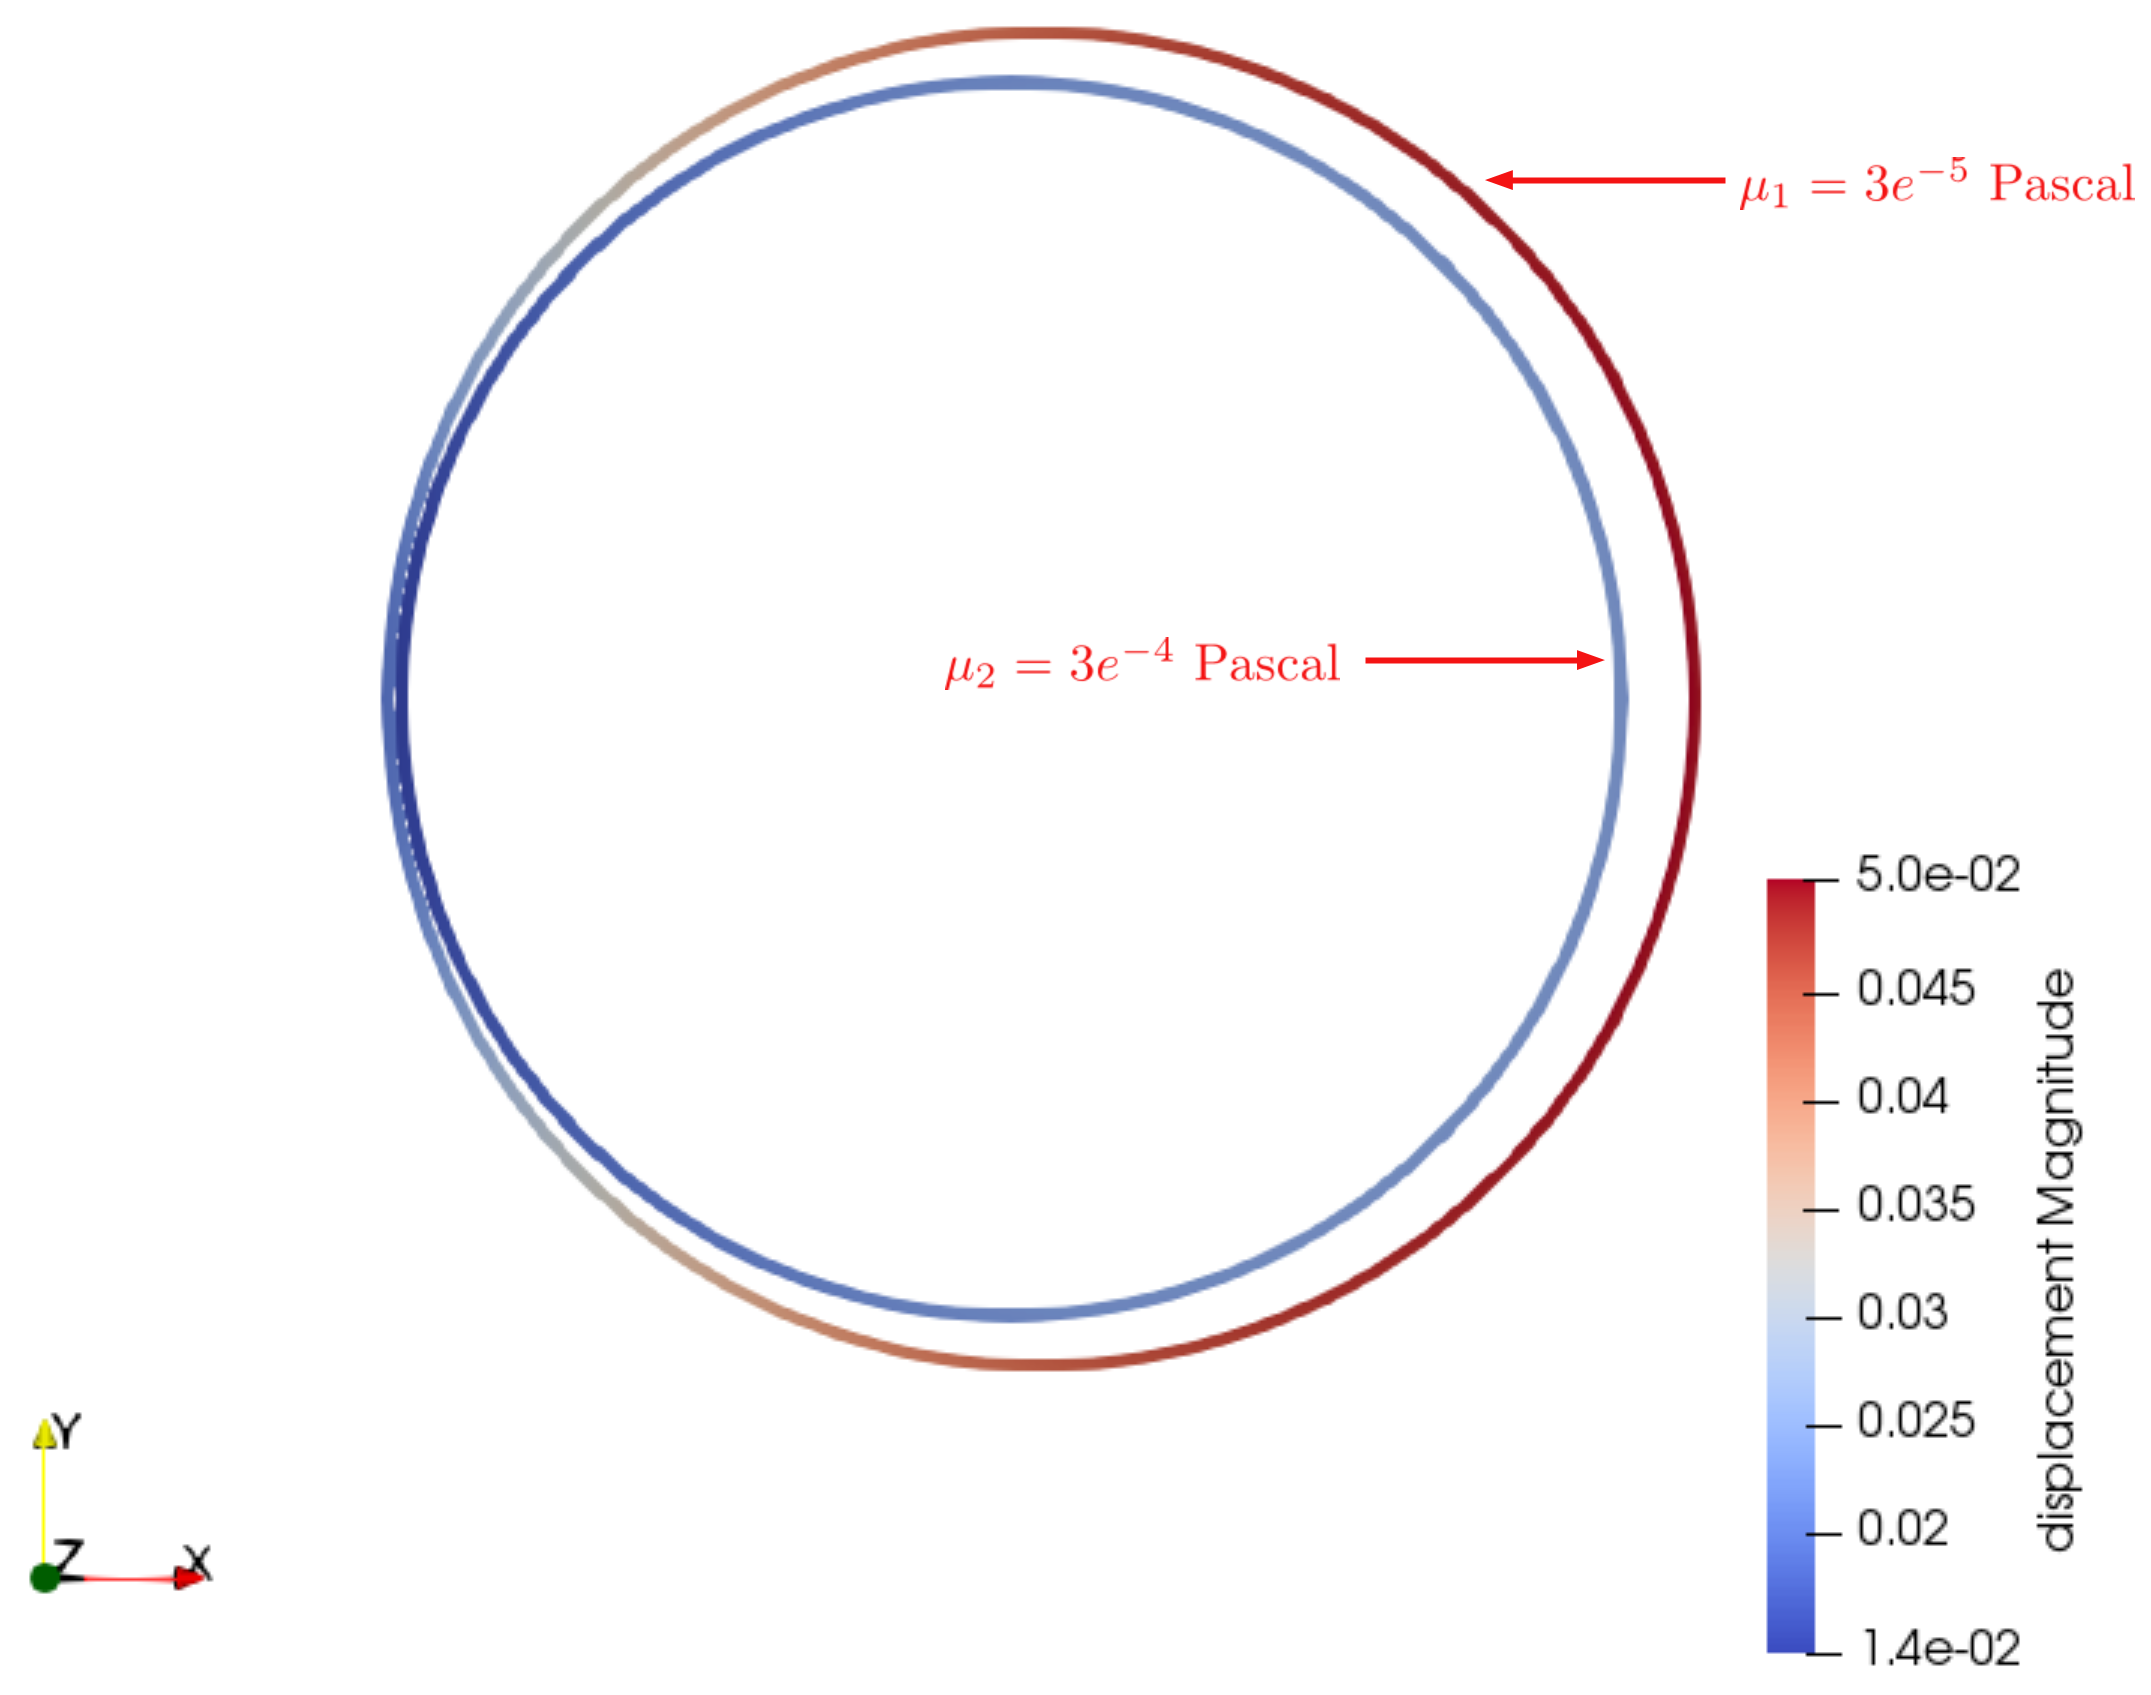
\includegraphics[width=0.9\textwidth]{mue_study_half_load.png}
\caption{Load step 9 (Half load)}
\label{fig:1.12.1}
\end{subfigure}
\begin{subfigure}[b]{0.49\textwidth}
\centering
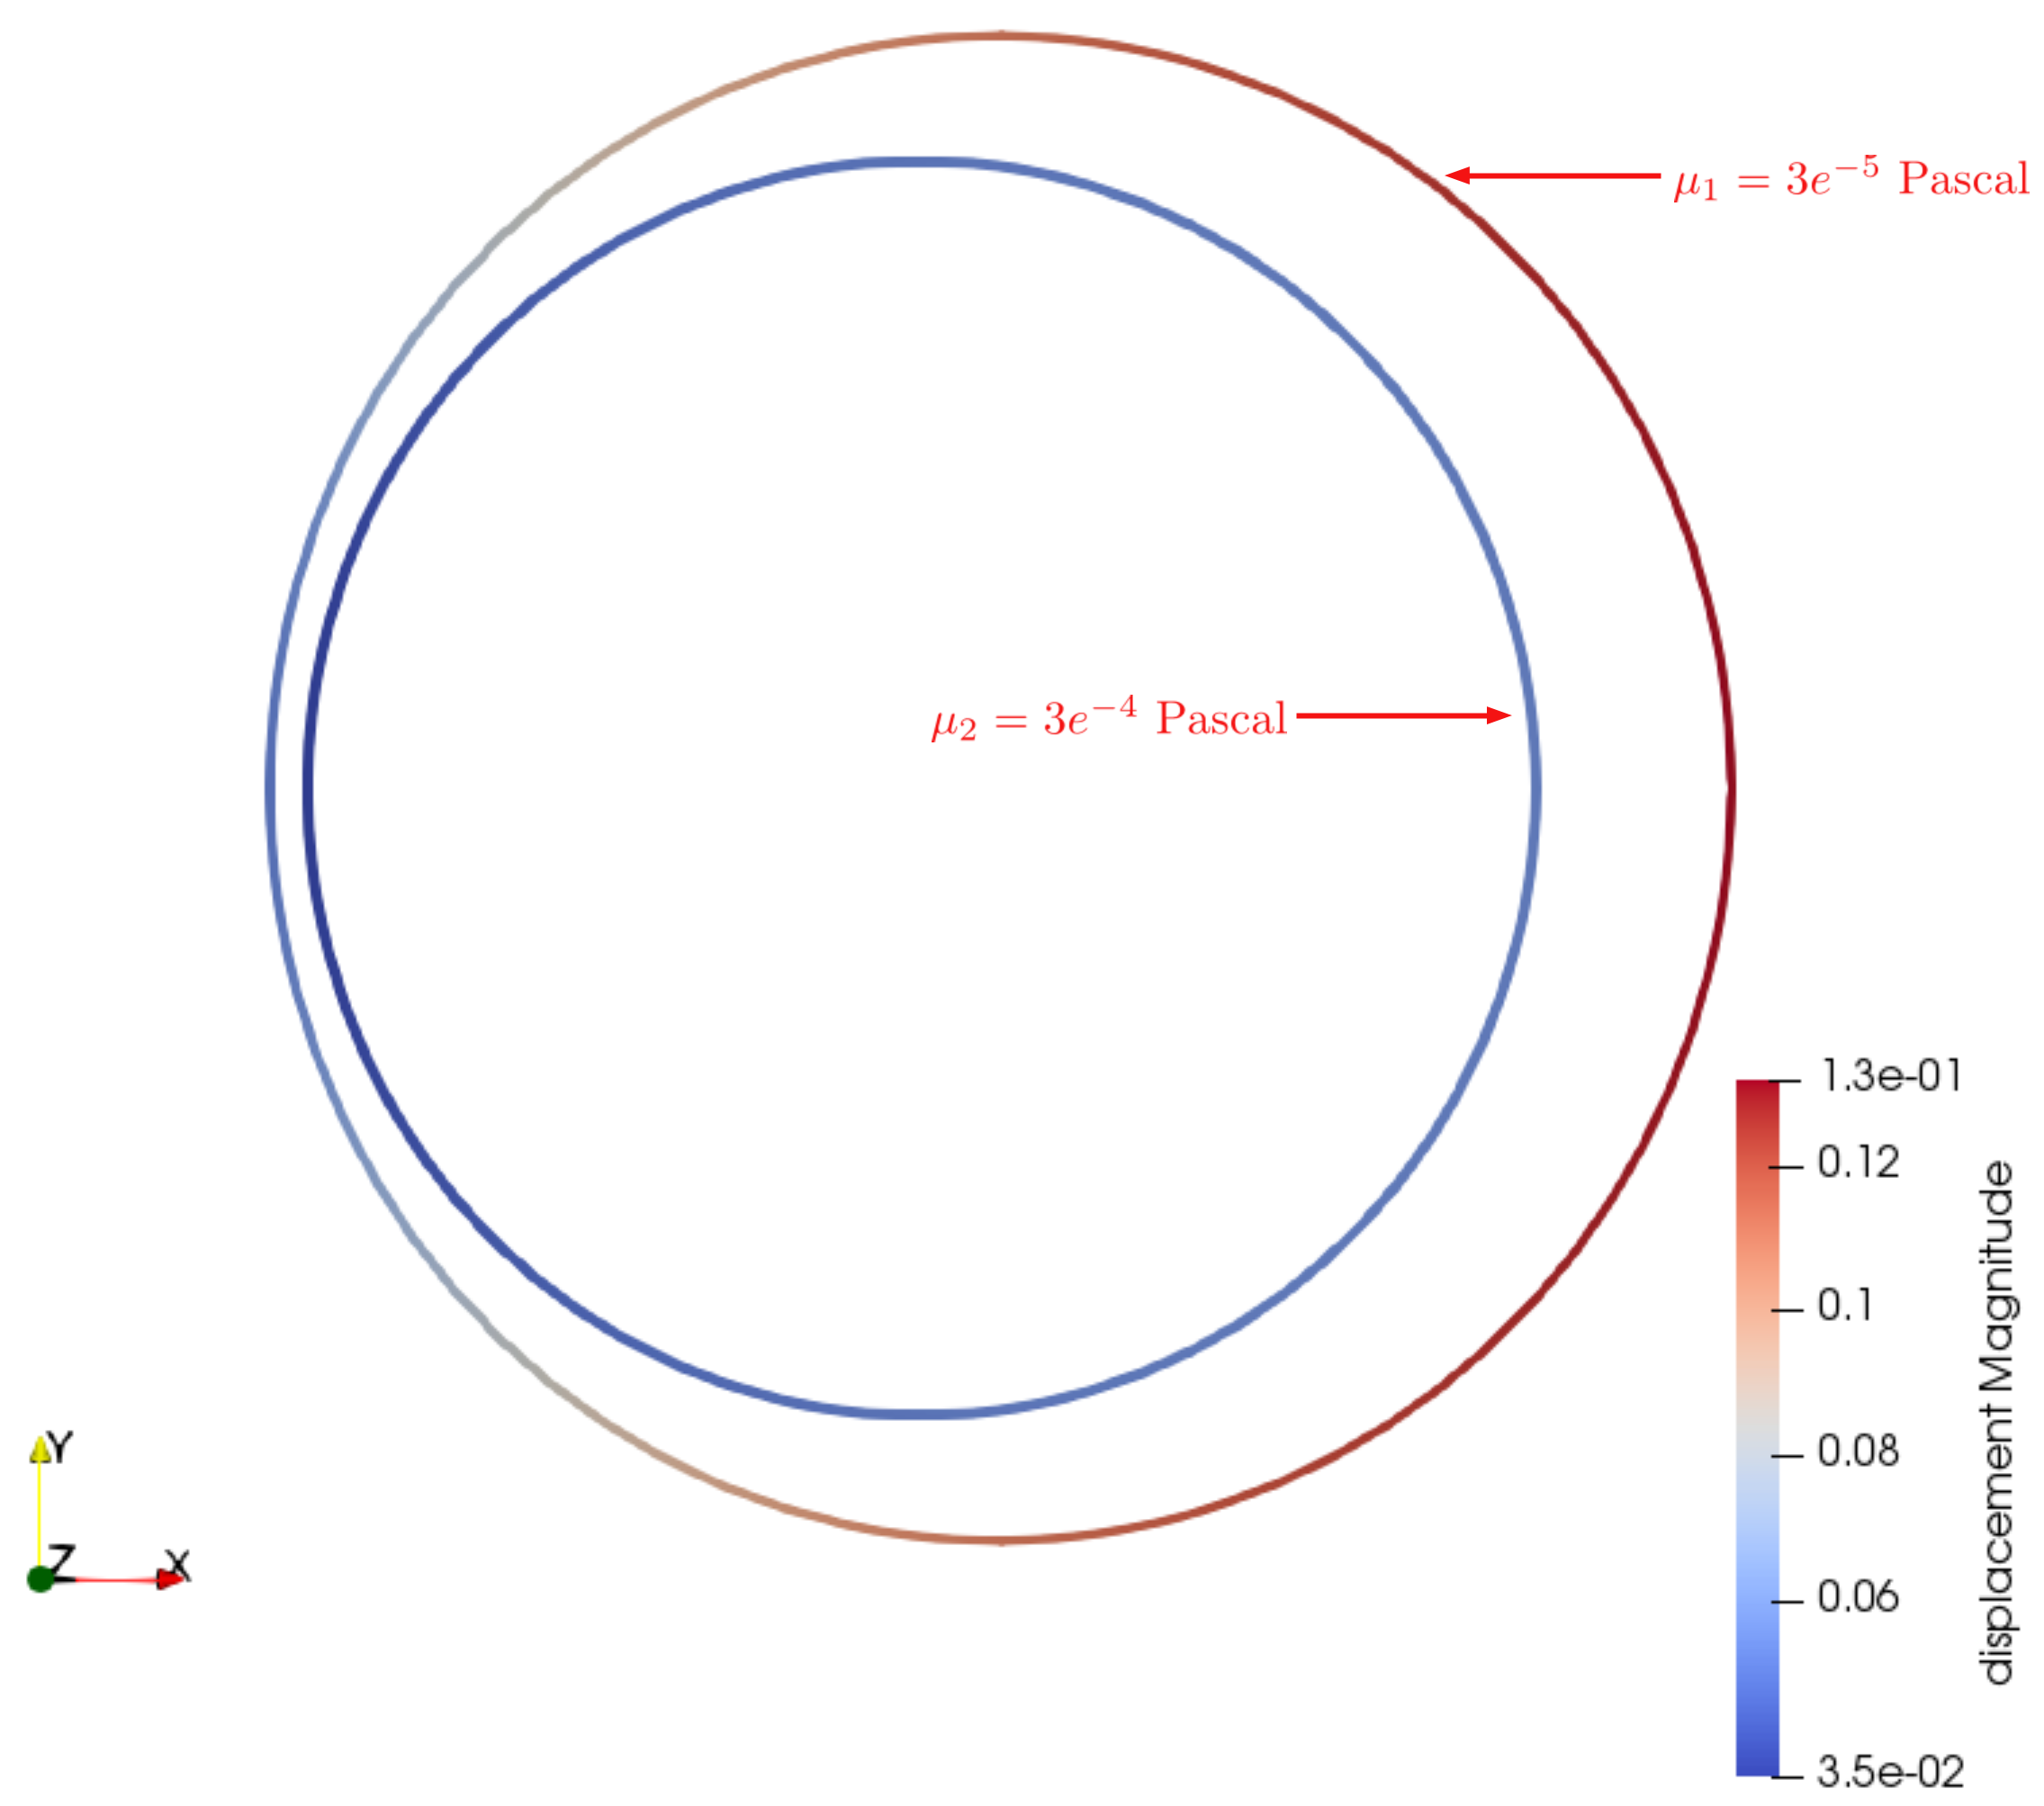
\includegraphics[width=0.9\textwidth]{mue_study_full_load.png}
\caption{Load step 19 (Full load)}
\label{fig:1.12.2}
\end{subfigure}
\caption{Deformations of torus membrane for different free space material parameter value $\mu$}
\label{fig:1.12}
\end{figure}

\begin{figure}[ht!]
\centering 
\begin{subfigure}[b]{0.49\textwidth}
\centering
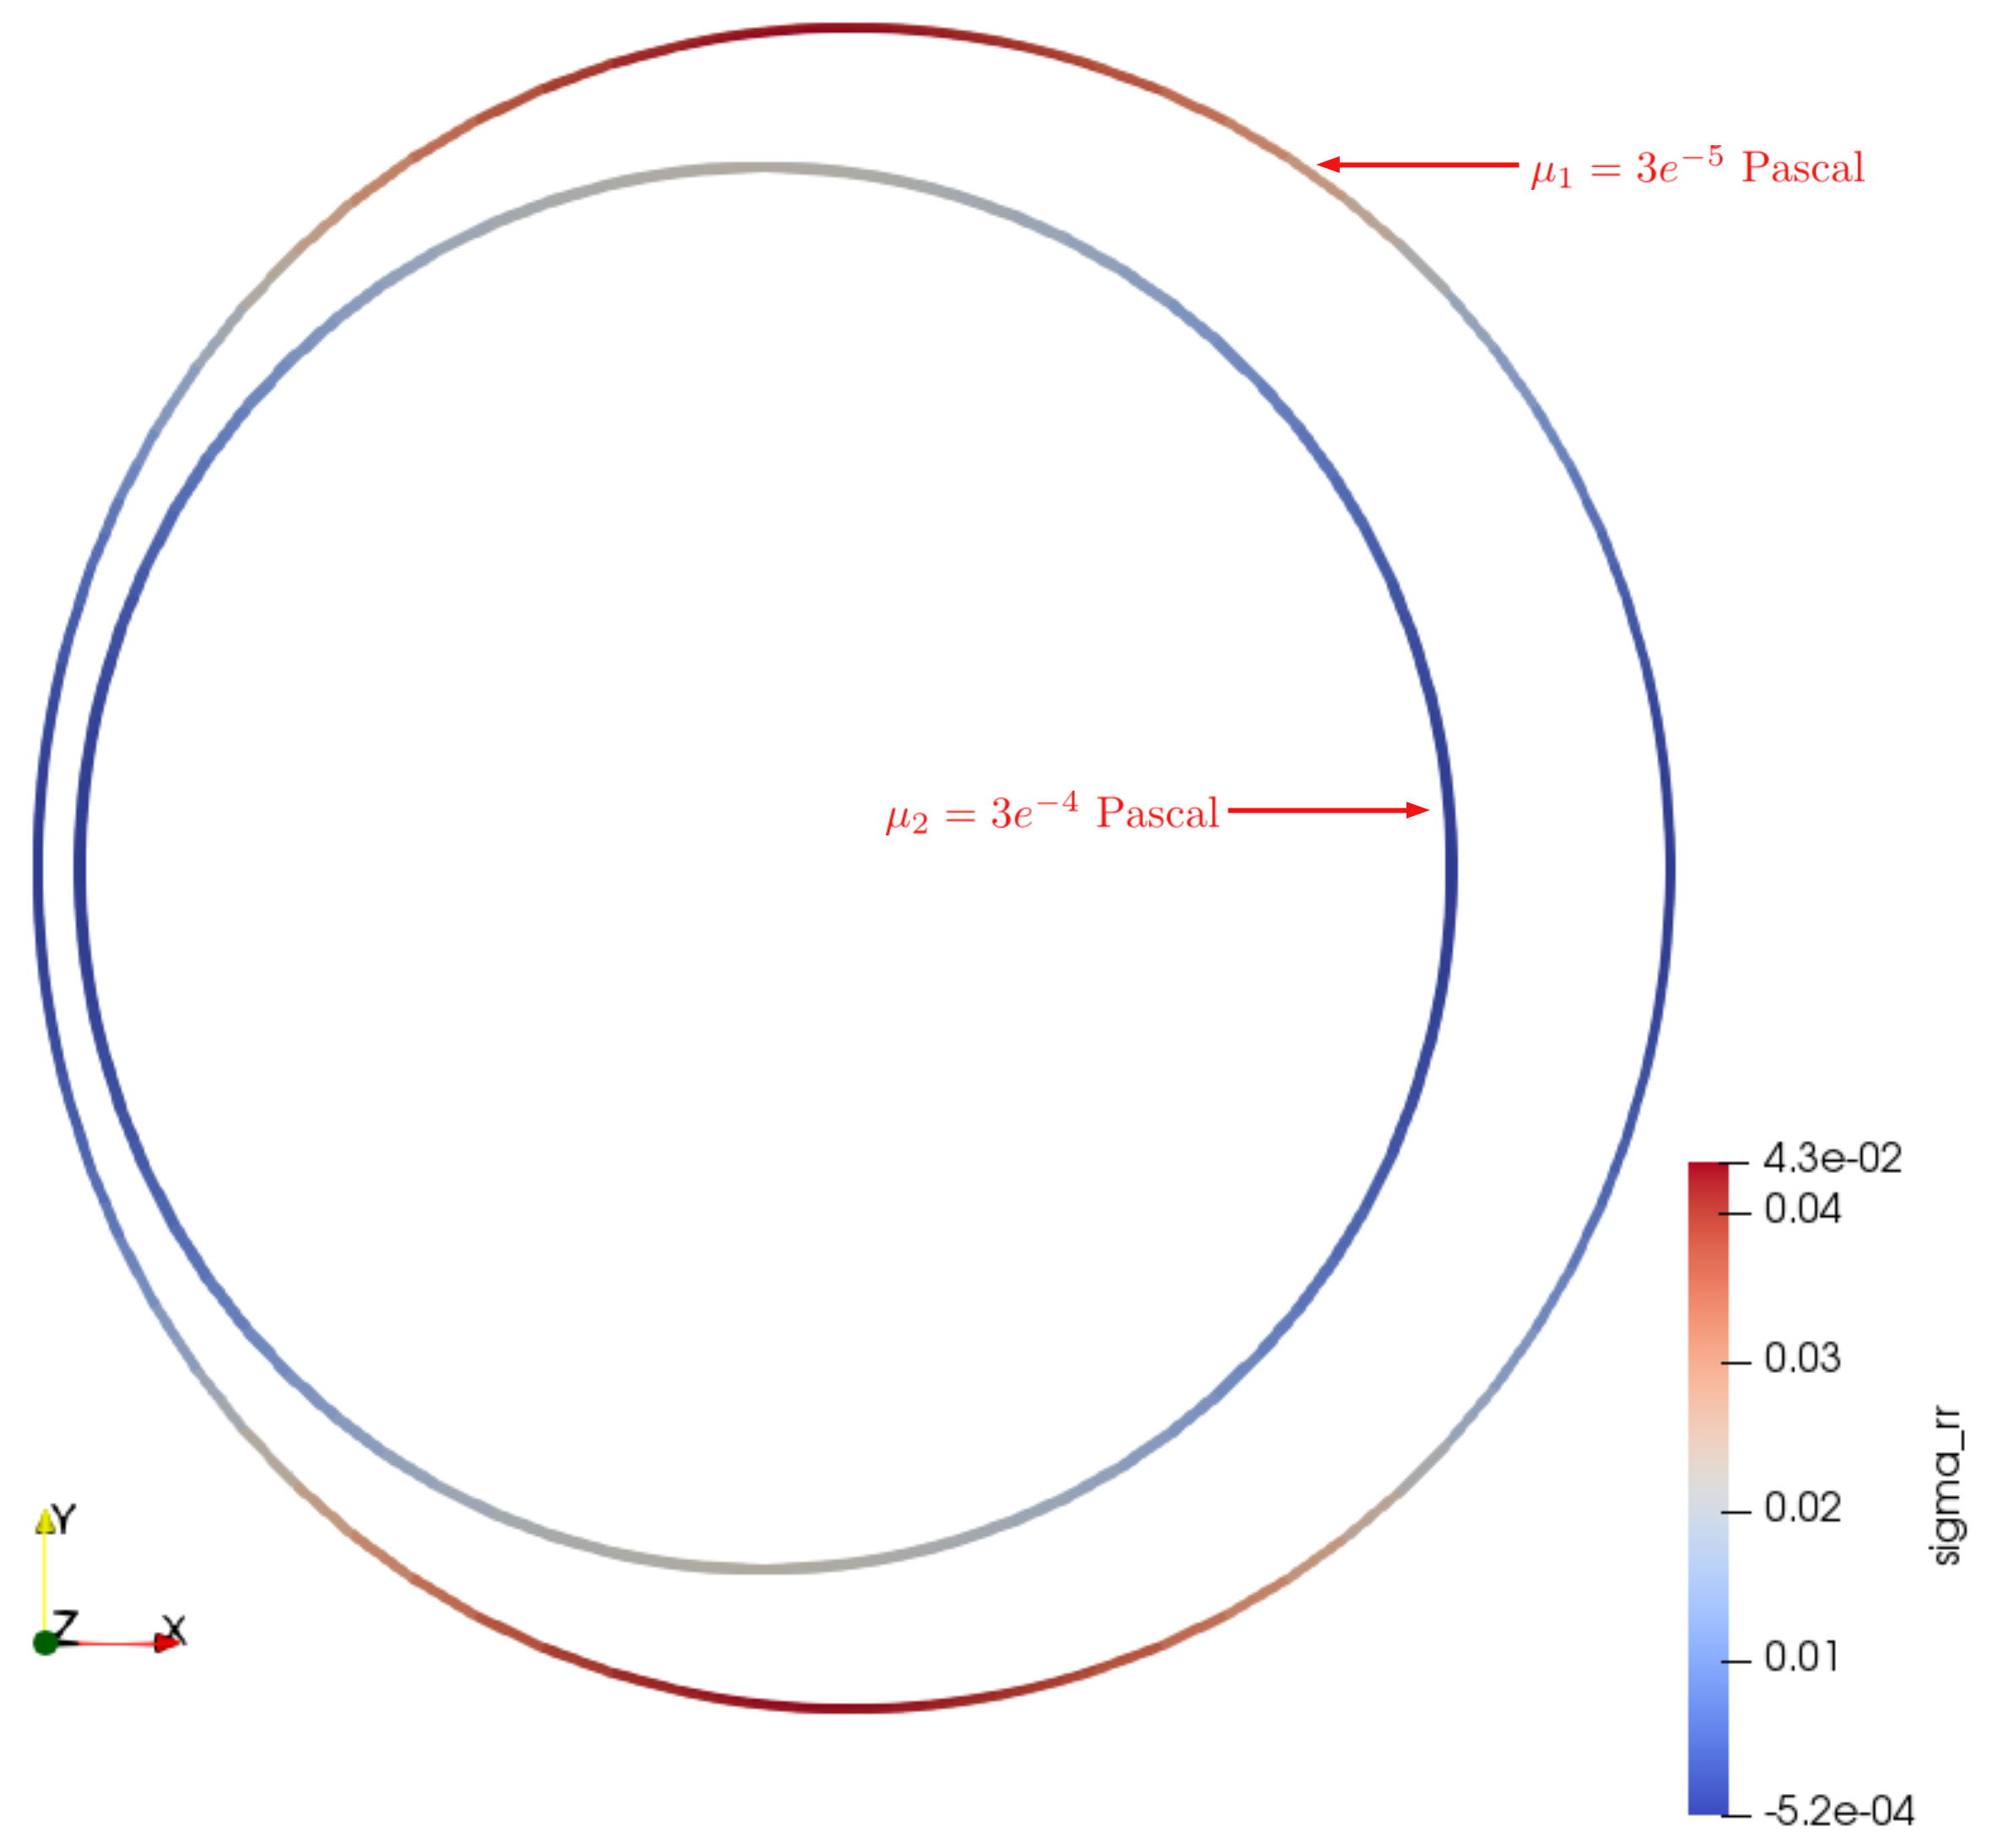
\includegraphics[width=0.9\textwidth]{torus_avg_sigma_rr.png}
\caption{$\sigma_{rr}$}
\label{fig:1.13.1}
\end{subfigure}
\begin{subfigure}[b]{0.49\textwidth}
\centering
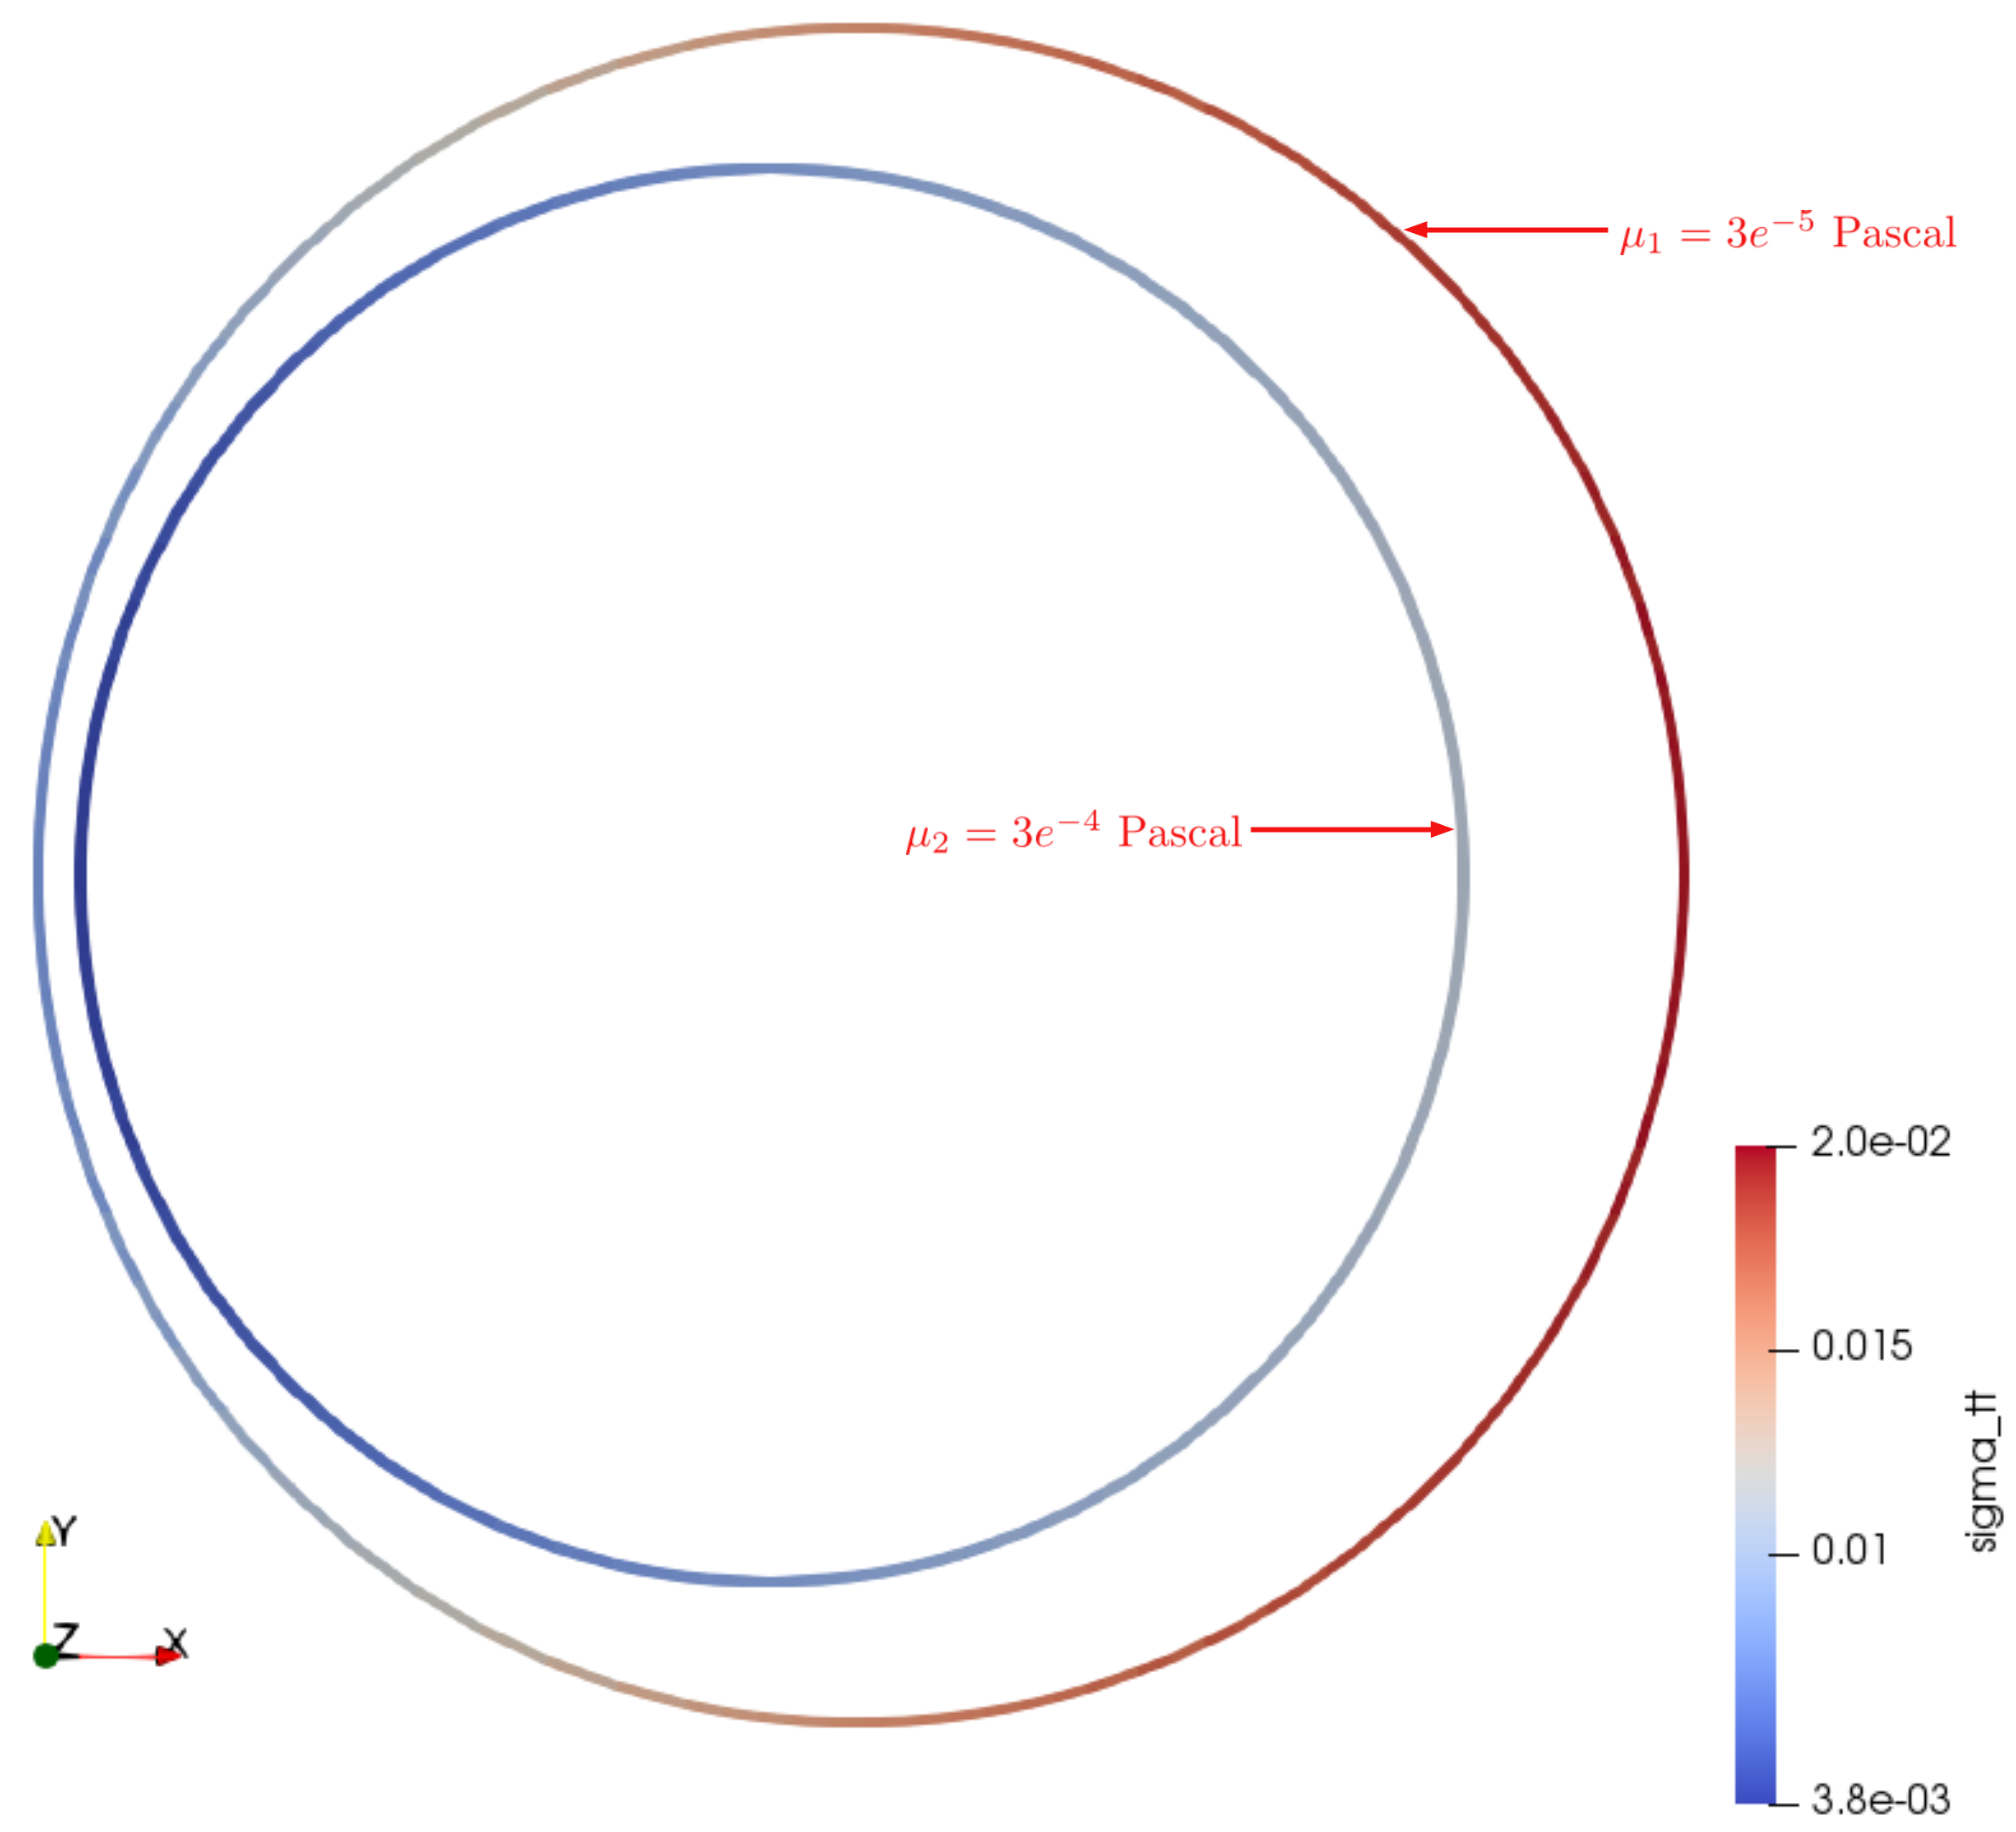
\includegraphics[width=0.9\textwidth]{torus_avg_sigma_theta.png}
\caption{$\sigma_{\theta \theta}$}
\label{fig:1.13.2}
\end{subfigure}
\caption{Element averaged Cauchy stress components of torus membrane for different free space material parameter value $\mu$}
\label{fig:1.13}
\end{figure}

\newpage
\subsection{\textbf{Vector-valued problem}} The solution in the elasticity problem discussed here is not just a single scalar function but has displacements $\mathbf{u} := \left\lbrace u_x, u_y, u_z \right\rbrace^T$ in each euclidean direction, thus we have a vector system which is a set of scalar functions and thus is also addressed as \textit{vector-valued solution}. When considering the coupled magneto-elastic problem (to be solved in next task), the resulting vector-valued solution we will solve for has elements $\left\lbrace \phi, u_x, u_y, u_z \right\rbrace^T$. These elements of the vector-valued solution can be grouped into \textit{blocks}, where for the coupled magneto-elastic problem we have two blocks at each global degree of freedom in the finite element mesh, one block for the magnetic scalar potential function $\phi$ and the second block for the vector displacement function $\mathbf{u}$ with three individual components $u_x, u_y, u_z$ in 3D. This way one is able to access all the components/elements of the vector field such as displacement together without splitting them into their individual components. 
\subsection{\textbf{Block linear algebra}} Use of the block structure also proves advantageous in terms of linear algebra and solution methods. One can think of the global linear system of equation $\mathbf{A}\mathbf{x} = \mathbf{b}$ as
\begin{equation*}
\begin{bmatrix}
\mathbf{A}_{\phi\phi} & \mathbf{0} \\
\mathbf{0} & \mathbf{A}_{\mathbf{u}\mathbf{u}} 
\end{bmatrix}
\begin{bmatrix}
\phi \\
\mathbf{u}
\end{bmatrix} 
= 
\begin{bmatrix}
\mathbf{F_{\phi}} \\
\mathbf{F_{\mathbf{u}}}
\end{bmatrix},
\end{equation*}
where $\phi$ and $\mathbf{u}$ are the values of the scalar magnetic potential field and the displacement field. $\mathbf{A}_{\phi\phi}$ denotes the matrix contributions arising from the linearization of the magnetic problem and $\mathbf{A}_{\mathbf{u}\mathbf{u}}$ describes the tangent matrix contribution from the elasticity problem. One can solve the complete system considering as a single unit which can be convenient for the assembly of the matrix and right-hand-side vector for some class of problems. When employing the Gauss elimination rather than solving the problem monolithically, depending upon the properties of the (block) matrices for individual problem one can then define individual preconditioners that best suite the operators present in the system of equations, rather than defining a single preconditioner for the global matrix $\mathbf{A}$.
\subsection{\textbf{Vector-valued Finite Elements}} We shall consider here in all the discussions only \textit{primitive finite elements}. A finite element is said to be primitive if there is a unique relation from the shape function number to the vector component of the vector-valued element. This means for a primitive element we have exactly one non-zero component for each shape function of the vector-valued element. The Lagrangian elements that we shall employ are primitive elements. For the considered vector-valued coupled magneto-elastic problem we build the vector-valued finite element from simpler base elements using tensor product of the base elements. We take multiple simple elements (eg. scalar linear Lagrange elements $Q_1$) and connect them to have an element with more than one block. For the vector-valued displacement field in 2D, we can construct a vector-valued finite element using two $Q_1$ elements (each constituting to a single component $u_x$ and $u_y$) to form using a tensor product $Q_1 \times Q_1$ element with two components. This will form a single block in our coupled problem where the second block for the scalar magnetic potential will have only a single component such as a quadratic element $Q_2$. Thus, the vector-valued element we shall employ, for e.g., can be represented in block form as ($Q_1 \times Q_1, Q_2$) which will have in total $\text{dim}+1$ individual components in 2D as [$u_x, u_y, \phi$]. \newline 

\newpage
\printbibliography
\end{document}
